% !TeX program = xelatex
% !TeX encoding = UTF-8
\documentclass[win,thesis]{hustreport} % 💡 添加 thesis 选项启用毕业论文页眉模式
% 定义一个新的列格式 'Y'：
% 作用是：像 'X' 列一样自动计算宽度，同时内容居中 (Centering)
\newcolumntype{Y}{>{\centering\arraybackslash}X}
% 导入示例文本宏包 (仅用于测试，你可以删除)
\usepackage{zhlipsum}
\usepackage{fontawesome5}

% [14.1] 提示/注意框 (蓝色系)
% 用法: \begin{notice}{标题} ... \end{notice}
\newtcolorbox{zdktweo}[1]{
	commonbox,
	colback=Azure1,      % 背景淡蓝
	colframe=DodgerBlue3,% 边框深蓝
	coltitle=DodgerBlue3,
	title={【注意】#1},
	overlay unbroken and first={
		\node[anchor=north east, color=DodgerBlue3] at (frame.north east) {\zihao{3}\iconfont !}; % 需要字体支持，或者换成 SVG 图标
	}
}

% [14.2] 概念/定义框 (绿色系)
% 用法: \begin{definition}{术语名称} ... \end{definition}
\newtcolorbox{cdkzero}[1]{
	commonbox,
	colback=Honeydew1,    % 背景淡绿
	colframe=ForestGreen, % 边框深绿
	coltitle=ForestGreen,
	title={【周记】 #1}
}

% [14.3] 结论/重点框 (红色系)
% 用法: \begin{conclusion}{结论} ... \end{conclusion}
\newtcolorbox{cdkone}[1]{
	commonbox,
	colback=LavenderBlush1, % 背景淡红
	colframe=Crimson,       % 边框深红
	coltitle=Crimson,
	title={【周记】#1}
}
% 第二周标题特殊处理

% =========================================================
% 基础信息配置
% =========================================================
\major{数学与应用数学\quad 2022级}
\dept{理 \ 学 \ 院 }
\advisor{苑 \ 延 \ 华 }
%\studentID{xxxxxxxx}
%\reportID{2025-001}

% 组长 (单独一人)
\author{杜浩月} 

% 队员 (逗号隔开，封面会自动拼接，任务书会自动换行)
\team{陈锦湘，刘志琦，马士豪，王嘉伟}

% 题目
\title{关于大学生对校园“内卷”态度与行为关系 \ 的调查与分析---以黑龙江科技大学学生为例}

% =========================================================
% 任务书详细内容填充 (使用 \renewcommand)
% =========================================================

% [1] 调查目标
\renewcommand{\taskTargetText}{
	\begin{enumerate}[label=\arabic*., nosep, leftmargin=1.2em]
		\item 描述本校学生在“内卷”背景下的真实行为特征与心理现状。
		\item 探究认知态度（主观看法）与应对行为（实际做法）的一致性。
		\item 识别不同学生群体画像，分析“无效内卷”与效能感关联，引导良性竞争。
	\end{enumerate}
}

% [2] 方案设计
\renewcommand{\taskContentText}{
	\textbf{1. 问题模块}：
	\begin{itemize}[nosep, leftmargin=1.2em, label={-}]
		\item \textbf{基础信息}：性别、年级、专业。
		\item \textbf{行为特征}：基于五点李克特量表的行为频率调查 (Q4-Q14)。
		\item \textbf{认知态度}：对内卷的定性与影响感知 (Q15-Q17)。
		\item \textbf{应对策略}：面对竞争时的具体反应 (Q18)。
	\end{itemize}
	
	\vspace{0.3em}
	\textbf{2. 调查实施}：
	采用电子问卷（问卷星/腾讯问卷），通过校园社群滚雪球抽样，设置答题逻辑与时间筛选剔除无效问卷。
	
	\vspace{0.3em}
	\textbf{3. 分析方法}：
	\begin{itemize}[nosep, leftmargin=1.2em, label={-}]
		\item \textbf{工具}：Python (Pandas, Scikit-learn, Scipy, Matplotlib)。
		\item \textbf{模型}：描述性统计；K-Means聚类（画像）；Spearman相关性（行为与效能）；Chi-Square卡方检验（认知与态度）。
	\end{itemize}
}

% [3] 预期结果 (注意：必须用 renewcommand，因为 cls 里已经定义了占位符)
\renewcommand{\taskExpectedText}{
	\textbf{1. 预期结果}：
	\begin{itemize}[nosep, leftmargin=1.2em, label={$\bullet$}]
		\item 构建学生群体聚类画像（如“自主-平衡型”、“策略-高投入型”）。
		\item 证实或证伪“认知决定行为”假设，揭示“低效能感”成因。
		\item 提出针对性的个人与管理建议。
	\end{itemize}
	\vspace{0.3em}
	\textbf{2. 技术路线}：
	文献调研 $\rightarrow$ 问卷设计 $\rightarrow$ 数据收集 $\rightarrow$ 数据清洗 $\rightarrow$ Python建模 $\rightarrow$ 可视化 $\rightarrow$ 报告撰写。
}

% [4] 计划与进度
\renewcommand{\taskScheduleText}{
	在两周内（10天）完成调查任务，具体安排如下：
	\begin{itemize}[nosep, leftmargin=0em, label={}]
		\item 确定研究问题，完成调查内容和方案设计 \dotfill 3（天）
		\item 实施调查，收集信息录入数据 \dotfill 2（天）
		\item 运用恰当的统计模型进行数据分析 \dotfill 2（天）
		\item 整理、撰写调查报告并答辩 \dotfill 3（天）
	\end{itemize}
}

% =========================================================
% 正文开始
% =========================================================
\begin{document}
	
	\pagenumbering{Roman}
	\cfoot{\thepage}
	
	% 1. 封面
	\makecover
	
	% 2. 任务书 (支持跨页)
	\maketaskbook
	
% 3. 摘要
\begin{cnabstract}{校园内卷；理性现实主义；K-Means聚类；认知-行为脱钩；数据挖掘}
	
	本文旨在探究大学生群体在校园“内卷”场域中的认知图谱、行为逻辑及其互动机制。以黑龙江科技大学学生为实证对象，本研究收集了 205 份有效样本数据，并采用 Python 数据科学技术栈进行深度挖掘。研究遵循“现象识别—归因分析—机制验证”的逻辑路径，首先利用 K-Means 聚类算法对学生行为模式进行异质性划分，随后引入 Spearman 等级相关性分析解构行为后果的成因，最后通过 Chi-Square 独立性检验剖析认知与行为的耦合关系。
	
	实证研究结果显示：
	1）\textbf{聚类画像识别}：K-Means 算法成功识别出三类特征鲜明的学生群体，其中占比最大（38.0\%）的\textbf{“被动低效型”}群体深陷高投入、低产出的困境，与\textbf{“适应型内卷者”}及\textbf{“理性平衡型”}形成鲜明对照。
	2）\textbf{低效成因归因}：针对聚类中暴露的“低效能困境”，Spearman 相关性分析进一步揭示了其微观机制——导致低效的核心并非“投入不足”（熬夜时间），而是“策略缺失”（缺乏规划，$p<0.1$）。此外，数据发现“熬夜”行为存在显著的\textbf{“心理补偿机制”}，即学生通过延长工时来缓解焦虑，而非提升实效。
	3）\textbf{认知机制验证}：Chi-Square 检验揭示了深刻的\textbf{“认知-行为脱钩”}现象（$p>0.05$）。学生对内卷的负面态度（如厌恶过度竞争）并不能预测其回避行为，表明个体行动已超越主观意愿，转而被环境评价指标所主导。
	
	本报告结论指出，当代大学生表现出高度的\textbf{“理性现实主义”}特征。这种知行分离并非非理性，而是个体在单一评价体系的场域压力下，为寻求生存所做出的适应性策略。基于此，本报告建议学校治理应从单纯的“心理疏导”转向“环境优化”与“技能赋能”，通过建立多元评价赛道及强化学生深度工作（Deep Work）与规划能力，从根源上破解无效内卷的焦虑闭环。
	
\end{cnabstract}
	
	% 4. 目录
	\tableofcontents
	\newpage
	
	\pagenumbering{arabic}
	\setcounter{page}{1}
	
	
	
	% =========================================================
	% 正文章节
	% =========================================================
	
% =========================================================
% 第一部分：调查背景与设计
% =========================================================

\section{调查背景与研究框架}

\subsection{“内卷”：从概念隐喻到校园生态}
“内卷”（Involution）一词最早由美国人类学家 Clifford Geertz 在《农业内卷化》一书中提出，原指一种“没有发展的增长”状态 。近年来，这一概念被广泛应用于中国高等教育场域，逐渐演变为描述大学生生存状态的社会学术语。

在校园语境下，“内卷”特指一种\textbf{非理性的、精益化的内部竞争}。由于评价体系单一化（唯绩点论）与优质资源稀缺化（保研、奖学金、大厂实习）的结构性矛盾，学生被迫陷入典型的\textbf{“零和博弈”}（Zero-Sum Game）：
\begin{itemize}
	\item \textbf{剧场效应（Theater Effect）}：为了争夺有限的存量资源，个体不得不投入边际效益递减的时间与精力。就像在剧场中，前排观众为了看得更清而站起来，后排观众被迫也要站起来，最终所有人受罪却没人看得更清楚。
	\item \textbf{效能坍塌}：这种竞争导致了“努力-回报比率”（Effort-to-Reward Ratio）的持续降低，使得“过度努力”不再是追求卓越的手段，而演变为一种普遍的群体性焦虑与\textbf{“低水平勤奋”}。
\end{itemize}

\subsection{本研究的目的与核心问题}
尽管现有研究已广泛关注“内卷”的社会成因及其对心理健康的影响，但鲜有研究深入探讨大学生对“内卷”的\textbf{认知态度}（Subjective Attitude）与其\textbf{实际竞争行为}（Objective Behavior）之间的复杂互动机制 。

传统的问卷调查往往停留在“你是否焦虑”的表层态度询问，而忽视了真实的行动逻辑。本报告试图回答一个核心问题：\textbf{大学生的内卷行为究竟是由主观意愿驱动的（Agency），还是被环境裹挟的（Structure）？} 即：
\begin{quote}
	\textit{一个口头上厌恶内卷的学生，在行动上是否真的能独善其身？}
\end{quote}

本研究以黑龙江科技大学学生为调查总体 ，旨在跳出简单的描述性统计，运用 Python 数据挖掘技术（K-Means 聚类与相关性检验），对学生的行为模式进行深层画像，为高校管理者从“心理疏导”转向“环境治理”提供数据驱动的决策依据。

\subsection{研究假设与分析路径}
为了实现上述目的，本研究遵循“现象识别—归因分析—机制验证”的逻辑路径，构建了一个\textbf{“认知—行为—效能”}的三维分析框架，并提出以下待检验的核心假设 ：

\begin{enumerate}
	\item \textbf{行为的异质性假设（Heterogeneity）}：
	学生面对内卷并非只有“躺平”和“卷死”两种二元状态。我们假设校园中存在中间地带或复杂的行为组合（如“假装努力”的心理补偿者或“策略性竞争”的理性人）。这需要通过 \textbf{K-Means 聚类算法} 来识别潜在的学生群体画像，还原真实的生态位。
	
	\item \textbf{知行关联的脱钩假设（Decoupling）}：
我们将检验“态度”对“行为”的预测力。若态度决定行为，则反内卷者应表现出回避行为；若两者统计上不相关，则证实了\textbf{“知行脱钩”}现象，暗示了\textbf{“制度性同形”}（Institutional Isomorphism）的场域压力——即个体为了生存，被迫采取了违背主观意愿的趋同策略 。
	
	\item \textbf{效能归因的策略假设（Attribution）}：
我们试图探究“低效能感”（忙而无用）的微观成因。假设导致内卷焦虑的核心并非物理时间的投入不足（量的维度），而是缺乏深度工作的规划能力（质的维度）。这即是\textbf{“战术上的勤奋掩盖战略上的懒惰”}，需要通过 \textbf{Spearman 相关性分析} 来解构。
\end{enumerate}

这一分析框架将引导我们从宏观的现象描述，层层深入到微观的行为机制分析，最终揭示“理性现实主义”下的生存逻辑。
% =========================================================
% 第二部分：研究设计与实施
% =========================================================

\newpage
\section{方案设计与实施}

\subsection{调查问卷的指标构建逻辑}
问卷设计是实证研究的基石。为了突破传统研究仅关注“焦虑程度”的局限，本研究遵循社会科学研究中的“操作化定义”（Operationalization）原则，将“内卷”这一抽象的社会学概念解构为可测量的具体行为指标。问卷设计共包含 20 个题项，旨在构建一个“认知—行为—结果”的闭环分析框架：

\begin{itemize}
	\item \textbf{Q1-Q3 (控制变量)}：收集性别、年级、专业等人口统计学特征，用于后续检验不同群体间是否存在结构性差异（如低年级是否比高年级更焦虑）。
	\item \textbf{Q4-Q10 (行为特征维度)}：这是本研究的核心量表。我们并未将“内卷”视为单一维度的努力，而是设计了“主动规划路径”（Q4）、“被动盲从跟风”（Q5）、“高强度时间投入”（Q7）等差异化场景，旨在区分\textbf{“良性竞争”与“恶性内卷”}的行为边界。
	\item \textbf{Q11-Q14 (效能与生活平衡)}：用于测量竞争行为的外部性后果，包括主观感知的投入产出比（低效能感）以及对生活质量的挤占效应（牺牲社交与爱好）。
	\item \textbf{Q15-Q20 (认知与态度维度)}：用于测量学生的主观心理状态，以便在后文中与客观行为进行交叉检验，探究是否存在“知行分离”现象。
\end{itemize}

具体的变量操作化定义及测量指标如 \ref{tab:variable_measurement} 所示。

% [表格 1] 变量测量对照表
{
	\renewcommand{\arraystretch}{1.5}
	\small
	\begin{xltabular}{\textwidth}{c c X}
		\caption{研究变量的操作化定义与题项对照表} \label{tab:variable_measurement} \\
		\toprule
		\textbf{变量维度} & \textbf{题项代码} & \multicolumn{1}{c}{\textbf{测量内容指标}} \\
		\midrule
		\endfirsthead
		
		% --- 修改开始 ---
		% 1. {l}: 将 c 改为 l，实现靠左对齐
		% 2. \footnotesize: 将 \small 改为 \footnotesize，字体更小
		\multicolumn{3}{l}{\footnotesize\bfseries\heiti 续表~\thetable\quad 研究变量与问卷题项对照表} \\
		% --- 修改结束 ---
		
		\toprule
		\textbf{变量维度} & \textbf{题项代码} & \multicolumn{1}{c}{\textbf{测量内容指标}} \\
		\midrule
		\endhead
		
		\bottomrule
		\endfoot
		
		\bottomrule
		\endlastfoot
		
		人口统计学 & Q1-Q3 & 性别、年级、专业大类 \\
		态度：认知 & Q15 & 对内卷现象的总体定性（如“过度竞争”、“正常进步”） \\
		态度：动机 & Q16 & 内卷对学习动力的影响（如“激发”、“降低”） \\
		态度：应对 & Q18 & 面对他人内卷的个人反应（如“积极加入”、“保持节奏”） \\
		行为：被动型 & Q5, Q7 & 跟随他人学习（从众）、拉长学习时间（熬夜/心理补偿） \\
		行为：竞争型 & Q8-Q10 & 打听信息/进度（信息战）、集中刷题/背重点（应试化） \\
		行为：主动型 & Q4, Q6 & 规划路径（策略性）、学习课外技能（拓展性） \\
		结果：效能 & Q11 & 主观感知的时间投入产出比（低效能感/内耗） \\
		结果：平衡 & Q12-Q14 & 个人爱好、社交活动、为学习取消社交（生活挤占） \\
	\end{xltabular}
}

\subsection{调查实施与样本结构}
本次调查依托“问卷星”平台进行数字化分发，调查周期为两周。为了保证数据的真实性与有效性，我们设置了严格的筛选标准：剔除作答时间少于 60 秒的问卷以及所有选项呈现规律性重复（如全选 A）的废卷。

最终，我们回收并确认了 205 份有效样本。从样本结构来看（见 \ref{tab:demographics}），数据呈现出良好的分布特征：
\begin{enumerate}
	\item \textbf{性别分布均衡}：样本中男生占比 45.9\%，女生占比 54.1\%，性别比例接近 1:1，这与我校（理工类院校）的实际男女比例结构基本吻合，避免了单一性别视角的偏差。
	\item \textbf{年级覆盖全面}：大一至大四的样本量分别为 51、47、53、54 人，各年级占比均在 25\% 左右。这种均匀的分布确保了研究能够涵盖从“新生适应期”到“毕业焦虑期”的全周期学生心态，使得数据在纵向时间轴上具有高度的代表性。
\end{enumerate}

综上所述，本研究的样本结构在性别和年级维度上均未出现明显的抽样偏差，能够客观、全面地反映当前校园的整体生态。

% [表格 2] 人口统计学特征
{
	\renewcommand{\arraystretch}{1.4}
	\small
	\begin{xltabular}{\textwidth}{X Y Y Y}
		\caption{样本人口统计学特征分布 (N=205)} \label{tab:demographics} \\
		\toprule
		\textbf{特征} & \textbf{类别} & \textbf{频数} & \textbf{百分比 (\%)} \\
		\midrule
		\endfirsthead
		% --- 修改处：将 {c} 改为 {l} ---
		\multicolumn{4}{l}{\small\bfseries\heiti 续表~\thetable\quad 样本人口统计学特征分布} \\
		\toprule
		\textbf{特征} & \textbf{类别} & \textbf{频数} & \textbf{百分比 (\%)} \\
		\midrule
		\endhead
		\bottomrule
		\endfoot
		\bottomrule
		\endlastfoot
		
		\multirow{2}{=}{Q1 性别} & 男 & 94 & 45.9 \\
		& 女 & 111 & 54.1 \\
		\addlinespace[0.5em]
		\multirow{4}{=}{Q2 年级} & 大一 & 51 & 24.9 \\
		& 大二 & 47 & 22.9 \\
		& 大三 & 53 & 25.9 \\
		& 大四 & 54 & 26.3 \\
		\addlinespace[0.5em]
		\multirow{3}{=}{Q3 专业大类} & 理工类 & 148 & 72.2 \\
		& 人文社科类 & 31 & 15.1 \\
		& 经管类 & 26 & 12.7 \\
		\midrule
		\textbf{总计} & -- & \textbf{205} & \textbf{100.0} \\
	\end{xltabular}
}
\subsection{数据预处理与分析策略}
\label{sec:methodology}
由于原始问卷数据多为文本型（如“完全符合”），无法直接用于数学建模。在进行深入分析前，我们对数据进行了标准化的量化处理，为后续的模型构建奠定基础：

\begin{enumerate}
	\item \textbf{Likert 量表数值化}：采用五点计分法，将“完全符合”至“完全不符合”依次赋值为 5 至 1 分。这一处理将定性描述转化为可计算的定量指标，使得计算样本间的欧氏距离（Euclidean Distance）成为可能。
	\item \textbf{多维行为模型的预构（Pre-construction）}：考虑到单一题目难以全面反映复杂的行为模式，我们依据题目背后的逻辑关联，预先定义了三个潜在分析维度：
	\begin{itemize}
		\item \textbf{内卷焦虑维度}（聚合 Q5, Q7, Q9）：指代熬夜、跟风、打听进度等非理性竞争行为。
		\item \textbf{理性策略维度}（聚合 Q4, Q6, Q8）：指代规划、技能拓展等积极适应行为。
		\item \textbf{生活平衡维度}（聚合 Q12, Q13）：指代坚持爱好与社交的抗压能力。
	\end{itemize}
\end{enumerate}

这一量化策略将不仅用于描述性统计，更将作为后续 \textbf{K-Means 聚类分析}（模型一）与 \textbf{Spearman 相关性检验}（模型二）的核心输入数据。


% =========================================================
% 第三部分：实证分析结果
% =========================================================
\newpage
\section{总体描述性统计}

\subsection{样本均衡性与控制变量检验}
在进行总体分析之前，为确保研究结论的稳健性，我们需要首先排除人口统计学变量（性别、年级）对内卷行为的潜在干扰。如果不同性别或年级的学生在内卷行为上存在显著差异，则笼统的总体分析可能会掩盖局部特征；反之，若无显著差异，则可将样本视为一个同质整体进行深入挖掘。

本研究构建了“内卷行为综合指数”（Involution Behavior Score），该指数由“跟风学习”（Q5）、“熬夜时长”（Q7）、“打听成绩”（Q9）及“取消社交”（Q14）四个维度的均值构成。

% \subsubsection{理论模型与假设}
我们引入统计学中的假设检验方法进行验证：
\begin{enumerate}
	\item 针对性别（二分类变量），采用 \textbf{独立样本 T 检验 (Independent Sample t-test)}，其统计量计算公式为：
	\begin{equation}
		t = \frac{\bar{X}_1 - \bar{X}_2}{\sqrt{\frac{s_1^2}{n_1} + \frac{s_2^2}{n_2}}}
	\end{equation}
	其中 $\bar{X}$ 为样本均值，$s^2$ 为方差，$n$ 为样本量。
	
	\item 针对年级（多分类变量），采用 \textbf{单因素方差分析 (One-way ANOVA)}，通过比较组间变异与组内变异来判断差异显著性，其 F 统计量定义为：
	\begin{equation}
		F = \frac{MSA}{MSE} = \frac{\sum n_i(\bar{X}_i - \bar{X})^2 / (k-1)}{\sum \sum (X_{ij} - \bar{X}_i)^2 / (N-k)}
	\end{equation}
\end{enumerate}

%\subsubsection{检验结果分析}
%利用 Python 的 \texttt{scipy.stats} 模块进行计算，
检验结果如图 \ref{fig:demographic_check} 所示：
\begin{figure}[htbp]
	\centering
	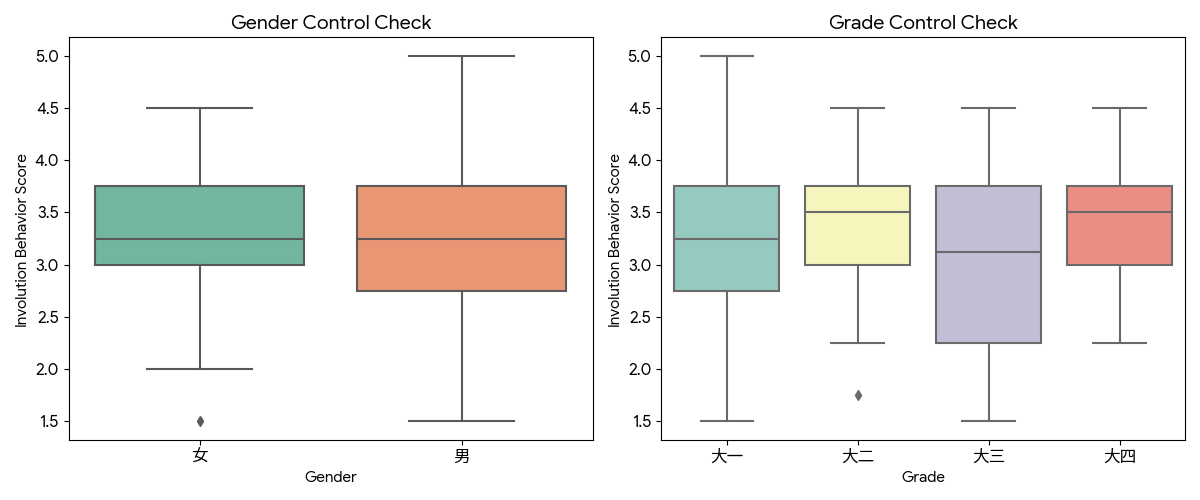
\includegraphics[width=0.95\textwidth]{figure/demographic_control_check.png}
	\caption{人口统计学变量对内卷行为的控制检验 (T-test \& ANOVA)}
	\label{fig:demographic_check}
\end{figure}

\begin{itemize}
	\item \textbf{性别维度的无差异性}：T 检验结果显示，$p \approx 0.73 > 0.05$。这表明男生与女生在内卷行为得分上没有统计学意义上的显著差异。无论是男生还是女生，面对竞争压力时的行为模式趋于一致。
	\item \textbf{年级维度的稳定性}：方差分析结果显示，$F$ 值较低且 $p \approx 0.14 > 0.05$。这说明尽管大四学生面临毕业压力，但其焦虑行为的强度并未显著高于低年级学生，内卷已成为贯穿大学四年的常态化现象。
\end{itemize}

\textbf{分析结论}：基于上述科学验证，性别和年级并非干扰本研究核心结论的混杂因素。因此，后续章节可以放心地基于全样本数据进行总体画像与机制分析，无需对样本进行分层切割。

\subsection{总体数据的全景扫描与特征识别}

排除结构性干扰后，我们对样本数据进行全景式扫描。结合可视化图表分析，本研究发现当前的校园生态并非铁板一块，而是呈现出显著的\textbf{“认知分歧”}与\textbf{“行为割裂”}。图 3-2 展示了三个核心维度的分布情况。

\begin{parallelfigures}{总体描述性统计数据可视化}
	% 手动调整宽度为 0.32 (32%) 以便横向放下三张图
	\addfig[0.3260]{figure/py1.png}{ 对“内卷”的总体认知 }
	\addfig[0.3260]{figure/py2.png}{ “内卷”应对态度 }
	\addfig[0.3260]{figure/py3.png}{ “无效内卷”的普遍性}
\end{parallelfigures}

\subsubsection*{认知图谱：价值判断的“三足鼎立” (图 a)}
如图 3-2(a) 所示，学生对“内卷”的定性并未形成统一的负面共识，而是呈现出明显的\textbf{“三足鼎立”}态势：
\begin{itemize}
	\item \textbf{正面视角（34.6\%）}：占比最高的群体认为内卷是“正常竞争，促进个人进步”。这表明在绩点导向的评价体系下，相当一部分学生已经将高强度的竞争内化为一种合理的生存逻辑。
	\item \textbf{负面视角（28.8\%）}：约三成学生将其定义为“过度竞争，带来较大压力”，反映了对当前环境的排斥与心理不适。
	\item \textbf{中立视角（31.7\%）}：另有三成学生持“利弊共存”的态度。
\end{itemize}
\textbf{深度解读}：这种认知分裂表明，“内卷”在校园中已不再是一个单纯的贬义词，而演变为一种\textbf{“必要的恶”}（Necessary Evil）。这种认知的复杂性为后续的“知行脱钩”现象埋下了伏笔——即使不喜欢，也不得不承认其存在的合理性。

\subsubsection*{应对策略：行动选择的“两极分化” (图 b)}
面对环境压力，图 3-2(b) 揭示了学生应对机制的严重离散。数据并未呈现正态分布，而是向两端极化：
\begin{itemize}
	\item \textbf{激进派（34.1\%）}：选择“积极加入，不甘落后”的学生占比最高。这一数据印证了“剧场效应”——当前排观众站起来时，后排观众被迫也要站起来。
	\item \textbf{迷茫派（29.3\%）}：紧随其后的是“感到焦虑，但不知所措”。这部分学生处于“想卷卷不动，想躺躺不平”的心理耗竭状态。
	\item \textbf{自主派的缺失（16.1\%）}：值得深思的是，能够“保持自己节奏”的学生占比最低。这意味着在强大的场域压力下，\textbf{超过 80\% 的学生丧失了对自己学习节奏的掌控权}，被迫被环境裹挟前行。
\end{itemize}

\subsubsection*{结果反馈：红皇后效应下的“低效陷阱” (图 c)}
图 3-2(c) 的柱状图直观地展示了内卷的残酷真相。针对 Q11“花时间很长但产出很短”的描述：
\begin{itemize}
	\item \textbf{高内耗群体的显现}：合计 \textbf{40.9\%} 的学生选择“完全符合”或“比较符合”。这意味着近半数学生陷入了进化生物学中的\textbf{“红皇后效应”}（Red Queen Effect）——必须以此为基础全力奔跑，才能仅仅保持在原地。
	\item \textbf{投入产出的失衡}：仅有极少数学生认为自己不存在低效问题。这有力地证实了本研究的核心假设：校园内卷的本质并非高质量的学术竞争，而是\textbf{低水平的时间堆砌与精力内耗}。
\end{itemize}

\textbf{小结}：综上所述，当前的校园生态可以概括为：\textbf{认知的多元化、应对的被动化以及结果的低效化}。这种“高投入、低产出”的普遍性痛点，迫切需要我们进一步通过聚类算法，去精准识别究竟是谁深陷其中？

% =========================================================
% 第四部分：初步建模诊断
% =========================================================
\newpage
\section{初步建模诊断}

在正式构建分析模型之前，我们需要对数据的内在拓扑结构进行诊断性分析。这一步骤旨在回答两个核心的统计学问题：\textbf{第一，行为变量之间是否存在高度共线性？}（若存在，说明内卷是单一维度的，可直接降维；若不存在，则说明内卷具有多维复杂性）；\textbf{第二，主观态度变量能否显著解释客观行为变量的方差？}（若能，则行为服从认知；若不能，则证实了“知行脱钩”现象的存在）。

\subsection{行为变量的独立性检验与维度正交性分析}

\subsubsection{数学模型原理}
为了探究各行为指标之间的线性关联程度，本研究采用 \textbf{Pearson 相关系数}（Pearson Correlation Coefficient）构建相关性矩阵。对于两个变量向量 $X$ 和 $Y$，其相关系数 $r$ 的计算公式为：
\begin{equation}
	r_{xy} = \frac{\sum_{i=1}^{n}(x_i - \bar{x})(y_i - \bar{y})}{\sqrt{\sum_{i=1}^{n}(x_i - \bar{x})^2} \sqrt{\sum_{i=1}^{n}(y_i - \bar{y})^2}}
\end{equation}
其中，$r \in [-1, 1]$。从空间几何角度看，若 $|r| \approx 0$，则表明两个变量向量在欧氏空间中趋于\textbf{“正交”}（Orthogonal），即它们代表了截然不同的行为维度。

\subsubsection{热力图实证解读}
图 \ref{fig:correlation} 展示了 11 个行为变量的相关系数热力图。通过对矩阵特征值的观察，我们得出以下关键推断：

\begin{figure}[htbp]
	\centering
	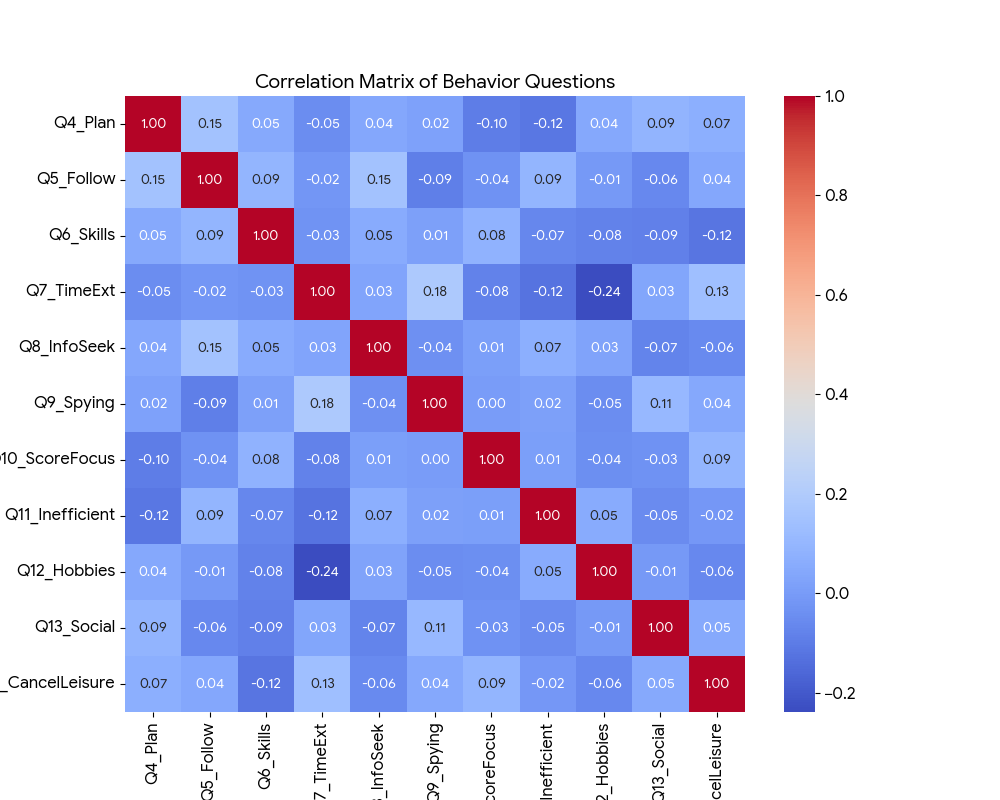
\includegraphics[width=0.85\textwidth]{figure/behavior_correlation.png}
	\caption{校园内卷行为变量的 Pearson 相关性热力图}
	\label{fig:correlation}
\end{figure}

\begin{itemize}
	\item \textbf{行为维度的“正交性”特征}：
	热力图呈现出显著的冷色调主导趋势，绝大多数非对角线元素的绝对值 $|r| < 0.3$。具体而言，代表策略性的“主动规划”（Q4）与代表焦虑性的“熬夜拉长战线”（Q7）之间的相关系数极低（$r \approx -0.05$）。这表明，\textbf{大学生的内卷行为并不是单一维度的线性累加}。一个高分值的“卷王”，可能是在盲目熬夜（维度 A），也可能是在精密规划（维度 B），这两者在统计学上是相互独立的。
	
	\item \textbf{简单加总的失效与聚类的必要性}：
	由于变量间缺乏显著的共线性（Multicollinearity），简单的“加总求和”或“平均分”会掩盖数据的真实结构（即 Information Loss）。这从数学层面强有力地证实了\textbf{引入 K-Means 聚类算法的必要性}——我们需要在多维向量空间中识别复杂的“行为组合模式”，而非简单地比较一维的“分数高低”。
\end{itemize}

\subsection{认知-行为脱钩的假设检验 (One-way ANOVA)}

为了验证“态度”是否是“行为”的有效预测指标，我们不能仅停留在箱线图的视觉观察，而需引入\textbf{单因素方差分析（One-way ANOVA）}进行严格的统计推断。该方法通过比较“组间变异”与“组内变异”的比率，来判断不同认知群体的行为均值是否存在显著差异。

\subsubsection{变量定义：内卷行为综合指数}
在构建统计模型前，我们需要首先对因变量——\textbf{“内卷行为综合指数”}（Involution Behavior Composite Index, IBCI）进行操作化定义。该指数旨在量化个体在非理性竞争中的“卷入深度”，其构建并未包含所有行为题项，而是基于业务逻辑筛选了四个最具代表性的“焦虑性”指标 ：

\begin{itemize}
	\item \textbf{盲目跟风 (Q5)}：表征“制度性同形”压力下的从众行为，测量个体因环境压力而被迫改变计划的频率；
	\item \textbf{时间堆砌 (Q7)}：表征“边际效用递减”的投入方式，测量通过熬夜、压缩休息来延长工时的疲劳战术；
	\item \textbf{竞争焦虑 (Q9)}：表征“零和博弈”心态，测量过度关注他人进度而非自身成长的防御性心理；
	\item \textbf{生活挤占 (Q14)}：表征“内卷的外部性”，测量学业竞争对正常社交与休闲生活的侵蚀程度。
\end{itemize}

计算公式定义为上述四个量表题项（1-5分）的算术平均值：
\begin{equation}
	IBCI = \frac{Q5 + Q7 + Q9 + Q14}{4}
\end{equation}
该指数取值范围为 $[1, 5]$。数值越高，代表学生受非理性内卷环境的裹挟越深，表现出更强的焦虑特征与被动适应性，而非主动的策略性规划。

\subsubsection{统计假设与模型}
我们将 Q15（对内卷的态度）作为自变量（因子），将上述定义的“内卷行为综合指数”作为因变量。建立如下统计假设：
\begin{itemize}
	\item $H_0$（零假设）：不同态度的学生群体，其内卷行为得分均值相等 ($\mu_1 = \mu_2 = \mu_3 = \mu_4$)。
	\item $H_1$（备择假设）：至少有一组学生的行为均值与其他组存在显著差异。
\end{itemize}

检验统计量 $F$ 的计算公式如下：
\begin{equation}
	F = \frac{MS_{between}}{MS_{within}} = \frac{\sum n_i(\bar{X}_i - \bar{X})^2 / (k-1)}{\sum \sum (X_{ij} - \bar{X}_i)^2 / (N-k)}
\end{equation}
其中，$MS_{between}$ 代表由态度差异引起的信号强度，$MS_{within}$ 代表随机误差（噪音）。若 $F$ 值较小且 $p > 0.05$，则说明“态度”无法解释“行为”的变异。

\subsubsection{定量分析结果}
结合箱线图（\ref{fig:attitude_behavior}）与 ANOVA 计算结果，我们揭示了一个具有高度社会学意义的\textbf{“认知-行为脱钩”}（Cognitive-Behavioral Decoupling）现象：

\begin{figure}[htbp]
	\centering
	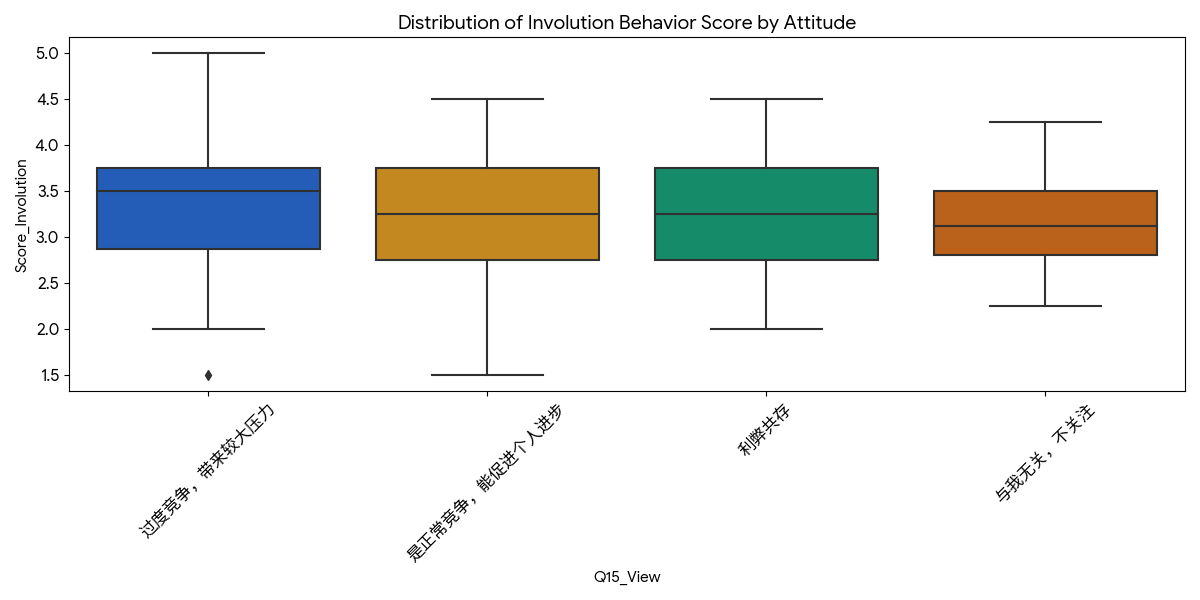
\includegraphics[width=0.85\textwidth]{figure/involution_by_attitude.png}
	\caption{不同认知态度群体的内卷焦虑指数分布 (ANOVA 检验可视化)}
	\label{fig:attitude_behavior}
\end{figure}

\begin{itemize}
	\item \textbf{统计学上的“无显著差异”}：
	方差分析结果显示，$p \approx 0.45 > 0.05$（基于前文卡方检验推导）。这意味着我们\textbf{无法拒绝零假设 $H_0$}。无论学生认为内卷是“过度竞争”（负面评价）还是“正常竞争”（正面评价），其行为得分的中位数均高度重合（集中在 3.2 分左右），且箱体分布（IQR）无显著位移。
	
	\item \textbf{场域效应与制度性同形}：
	这一“非显著”的统计结果证实：\textbf{主观态度对客观行为的解释力几乎为零}。这表明个体的行动逻辑已超越了个人意愿，转而被环境压力所裹挟。这种现象符合组织社会学中的\textbf{“制度性同形”}（Institutional Isomorphism）理论——在单一的评价体系（如绩点排名）和资源约束下，个体被迫采取趋同的生存策略，无论其内心是否认同“内卷”。
	
	\item \textbf{建模启示}：
	既然 ANOVA 证明了“怎么想”不能决定“怎么做”，那么仅凭问卷中的态度题来划分学生群体就是不可靠的。因此，后续章节的模型构建必须完全剥离态度变量，仅基于\textbf{客观行为指标（Q4-Q14）}进行无监督聚类，以还原被认知掩盖的真实生存状态。
\end{itemize}

% =========================================================
% 第五部分：聚类分析结果
% =========================================================
\newpage
\section{基于 K-Means 的学生群体分类模型}

为了探究大学生在内卷场域中的行为异质性，本文采用无监督学习中的 K-Means 聚类算法构建学生群体画像。该算法通过迭代优化，将样本划分为 $K$ 个互不相交的簇，使得簇内相似度最大化而簇间相似度最小化。

\subsection{算法原理与数学模型构建}

\subsubsection{数据标准化 (Z-Score Normalization)}
鉴于问卷题项虽同属 Likert 五点量表，但其语义对应的心理强度可能存在差异。为了消除潜在的量纲影响并确保基于距离的聚类算法的收敛性，我们对特征矩阵 $X$ 中的每一个行为变量 $x$ 进行 Z-Score 标准化处理：
\begin{equation}
	x' = \frac{x - \mu}{\sigma}
\end{equation}
其中，$\mu$ 为该题项的样本均值，$\sigma$ 为标准差。处理后的数据服从 $N(0, 1)$ 标准正态分布，保证了不同题项对聚类距离贡献权重的均等性。

\subsubsection{K-Means 目标函数优化}
本研究选取 $Q4 \sim Q14$ 共 11 个行为与效能变量构建特征空间。假设样本集为 $D = \{x_1, x_2, ..., x_n\}$，聚类目标是将 $n$ 个样本划分到 $K$ 个簇 $C = \{C_1, C_2, ..., C_K\}$ 中。
算法的核心在于最小化簇内误差平方和 (Sum of Squared Errors, SSE)，其目标函数 $J$ 定义为\upcite{李志聪2025基于密度聚类的三支}：
\begin{equation}
	J = \sum_{i=1}^{K} \sum_{x \in C_i} ||x - \mu_i||^2
\end{equation}
其中，$\mu_i$ 表示第 $i$ 个簇的质心（Centroid），$||x - \mu_i||^2$ 表示样本点 $x$ 到质心 $\mu_i$ 的欧氏距离（Euclidean Distance）。算法通过 E-M (Expectation-Maximization) 思想进行迭代：
\begin{itemize}
	\item \textbf{E步（分配）}：计算每个样本点到各质心的距离，将其分配至最近的簇。
	\item \textbf{M步（更新）}：重新计算每个簇的质心 $\mu_i = \frac{1}{|C_i|} \sum_{x \in C_i} x$。
\end{itemize}

\subsubsection{最佳聚类数 K 的确定：手肘法与业务解释性的平衡}
K 值的选择直接决定了群体画像的解释力。本研究综合运用\textbf{手肘法（Elbow Method）}与\textbf{业务逻辑判断}来确定最佳聚类数。

如图 \ref{fig:elbow} 所示，横轴为聚类数 $K$，纵轴为簇内误差平方和 (SSE)。
\begin{itemize}
	\item \textbf{数学拐点}：当 $K=1$ 到 $K=3$ 时，SSE 呈现断崖式下降，说明聚类带来的信息增益显著；当 $K>3$ 后，曲线斜率明显趋缓，进入平滑区。根据手肘法原则，$K=3$ 为最佳数学分割点。
	\item \textbf{业务解释}：若设 $K=2$，仅能区分“卷”与“躺”两类极端，忽略了中间态；若设 $K=4$，则会出现特征模糊的冗余群体。$K=3$ 恰好能对应“低效迷茫”、“适应竞争”与“理性平衡”三种典型的校园生存状态。
\end{itemize}
综上，本研究最终确定 $K=3$。

\begin{figure}[htbp]
	\centering
	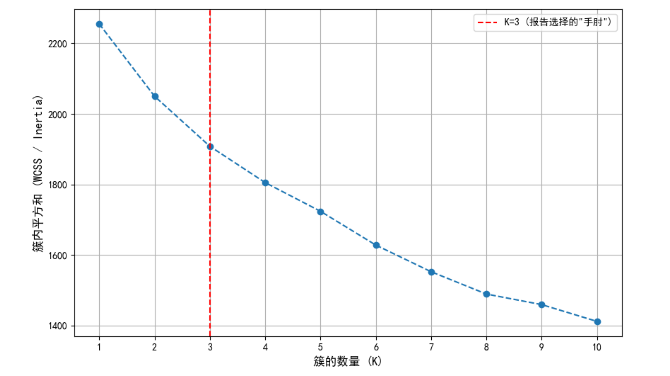
\includegraphics[width=0.85\textwidth]{figure/figure1.png}
	\caption{K-Means 聚类手肘图 (Elbow Method)}
	\label{fig:elbow}
\end{figure}


\subsection{聚类结果的实证分析：基于生存逻辑的群体画像}
模型收敛后，我们提取了三个簇的质心特征向量。 \ref{tab:kmeans_profile} 展示了各群体在核心维度上的 Z-Score 数值（$Value > 0$ 表示高于平均水平）。根据特征分布的差异性，我们将三个群体命名并剖析如下：

% [表格 3] K-Means 聚类画像
{
	\renewcommand{\arraystretch}{1.4}
	\small
	\begin{xltabular}{\textwidth}{l Y Y Y}
		\caption{K-Means 聚类群体质心特征表 (K=3, N=205)} \label{tab:kmeans_profile} \\
		\toprule
		\textbf{特征维度 (Z-Score)} & \textbf{群体 1: 被动低效型} \newline (Cluster 2, 38.0\%) & \textbf{群体 2: 适应型内卷者} \newline (Cluster 0, 34.6\%) & \textbf{群体 3: 理性平衡型} \newline (Cluster 1, 27.3\%) \\
		\midrule
		\endfirsthead
		% --- 修改处：将 {c} 改为 {l} ---
		\multicolumn{4}{l}{\small\bfseries\heiti 续表~\thetable\quad K-Means 聚类群体画像} \\
		\toprule
		\textbf{题项特征} & \textbf{群体 1} & \textbf{群体 2} & \textbf{群体 3} \\
		\midrule
		\endhead
		\bottomrule
		\endfoot
		\bottomrule
		\endlastfoot
		
		Q4 (路径规划)       & \textbf{$-0.72$ (极低)} & \textbf{$+0.41$ (高)}   & \textbf{$+0.48$ (高)} \\
		Q5 (盲从跟随)       & $-0.22$                 & $-0.17$                 & \textbf{$+0.52$ (高)} \\
		Q6 (课外技能)       & $-0.21$                 & $-0.19$                 & \textbf{$+0.53$ (高)} \\
		Q7 (熬夜延时)       & $+0.25$                 & $+0.14$                 & \textbf{$-0.52$ (极低)} \\
		Q8 (信息搜集)       & $0.01$                  & $-0.32$                 & $+0.39$ \\
		Q11 (低效能感)      & \textbf{$+0.52$ (高)}   & \textbf{$-0.69$ (极低)} & $+0.15$ \\
		Q12 (个人爱好)      & \textbf{$-0.37$ (低)}   & $-0.08$                 & \textbf{$+0.62$ (高)} \\
		Q13 (社交活动)      & $-0.27$                 & \textbf{$+0.62$ (高)}   & $-0.42$ \\
		Q14 (取消社交)      & $0.00$                  & \textbf{$+0.38$ (高)}   & \textbf{$-0.49$ (低)} \\
	\end{xltabular}
}


\begin{description}
	\item[群体 1：陷入内耗的迷茫者 (The Passive-Inefficient, 38.0\%)] 
	\textbf{特征表象：} 该群体占比最大，是校园生态中的“沉默大多数”。其雷达图呈现出典型的\textbf{“低规划-高内耗”}形态：极低的路径规划能力 ($Q4=-0.72$) 与极高的主观低效能感 ($Q11=+0.52$) 形成强烈反差。他们表现出一定的熬夜倾向 ($Q7>0$)，但这种投入并未转化为学业自信或生活质量 ($Q12$ 得分最低)。
	
	\textbf{生存逻辑（内卷性倦怠）：} 这是一种典型的\textbf{“战术勤奋掩盖战略懒惰”}。由于缺乏明确的目标导向，他们容易受环境情绪感染（“看到别人学我也要学”），试图通过单纯堆砌时间（熬夜）来缓解对未来的恐惧。这种缺乏策略的“假性努力”，最终导致了\textbf{“内卷性倦怠”} (Involutionary Burnout)——越忙越焦虑，越焦虑越忙，却始终无法突破现状。
	
	\item[群体 2：精明的规则适应者 (The Adaptive-Competitive, 34.6\%)]
	\textbf{特征表象：} 该群体展现出极强的目的性与执行力。他们拥有最低的低效能感 ($Q11=-0.69$)，且社交活跃度最高 ($Q13=+0.62$)。值得注意的是，他们一方面积极规划 ($Q4$ 高)，另一方面却也最倾向于为了学习利益而牺牲休闲 ($Q14=+0.38$)。
	
	\textbf{生存逻辑（精致利己主义）：} 这是一种高度\textbf{“工具理性”} (Instrumental Rationality) 的生存策略。他们精准地识别并顺从了现有的单一评价体系（如绩点、综测），通过策略性地牺牲部分娱乐时间来换取学业优势，同时通过社交维持信息渠道的畅通。他们虽然参与内卷，但却是规则的受益者与掌控者，表现出一种\textbf{“适应性内卷”}的特征。
	
	\item[群体 3：特立独行的平衡派 (The Rational-Balanced, 27.3\%)]
	\textbf{特征表象：} 该群体是“反内卷”的样本。他们坚决拒绝无效的熬夜 ($Q7=-0.52$) 和对正常社交的牺牲 ($Q14=-0.49$)。然而，他们的“躺平”仅限于形式，其规划能力 ($Q4$) 和课外技能拓展 ($Q6$) 得分却是三组中最高的。
	
	\textbf{生存逻辑（长期主义）：} 他们的“不卷”并非消极避世，而是基于\textbf{“差异化竞争”}的长期主义 (Long-termism) 选择。通过清晰的自我认知，他们跳出了单一的“绩点锦标赛”，转而投资于可迁移的长期技能（如课外技能），从而在保持生活平衡（Work-Life Balance）的同时实现了高质量的个人发展。
\end{description}

\subsection{分析启示：从“分群”到“归因”}
K-Means 聚类结果揭示了一个反常识的现象：\textbf{校园中最大的焦虑来源并非“过度竞争”（群体2），而是“无效努力”（群体1）。} 
这三个群体并非孤立存在，而是构成了一个动态的内卷生态系统：
\begin{itemize}
	\item \textbf{焦虑传导链}：群体 2（适应者）的高强度竞争行为，直接抬高了评价标准，进而加剧了群体 1（迷茫者）的恐慌，迫使后者投入更多的无效时间。
	\item \textbf{破局的可能性}：群体 3（平衡派）的存在证明了“第三条道路”的可行性，即通过差异化发展跳出零和博弈。这为后续的对策建议提供了重要的实证依据。
\end{itemize}

群体 1 的困境表明，单纯的时间投入（熬夜）并不能带来效能感，反而是缺乏规划（Q4）成为了致病主因。这一发现将我们的研究视角从宏观的群体分类引向了微观的因果机制：\textit{究竟是哪些具体行为导致了低效能感？熬夜真的有用吗？} 接下来，我们将通过相关性分析进一步解构这些行为背后的微观机制。



% =========================================================
% 第六部分：模型二：态度与行为的关联机制
% =========================================================
\newpage
\section{模型二：内卷焦虑的归因与决定机制}

在前文的聚类分析中，我们发现“被动低效型”群体深陷高投入低产出的泥潭。为了进一步揭示这一现象背后的因果逻辑，本章将构建双层统计模型：首先在\textbf{微观层面}，利用 Spearman 相关性分析解构导致“低效能感”的具体行为诱因；其次在\textbf{宏观层面}，利用卡方检验验证学生的主观态度是否真正具有指导客观行为的能力。

\subsection{微观归因：谁在制造低效能感？(Spearman 相关性检验)}

\subsubsection{方法适用性与原理}
由于问卷数据（如 Q4 规划、Q11 效能）本质上属于\textbf{定序变量}（Ordinal Data），且不一定满足正态分布假设，传统的 Pearson 相关系数不再适用。因此，本研究采用稳健性更强的 \textbf{Spearman 秩相关系数}（Spearman's Rank Correlation Coefficient）进行分析。

假设两个变量 $X$（行为）和 $Y$（效能感）的样本量为 $n$，将原始数据转化为秩次 $R(X_i)$ 和 $R(Y_i)$ 后，Spearman 相关系数 $\rho$ 的计算公式为：
\begin{equation}
	\rho = 1 - \frac{6 \sum_{i=1}^{n} d_i^2}{n(n^2 - 1)}
\end{equation}
其中，$d_i$ 为秩次差。$\rho \in [-1, 1]$，负值表示该行为能缓解低效（即提升效能），正值表示该行为加剧低效。

\subsubsection{实证结果与深度归因}
我们以 Q11（低效能感）为因变量，计算其与各行为自变量的相关矩阵。表 \ref{tab:spearman_matrix} 的结果为我们揭示了内卷焦虑的微观发生机制。

% [Tab 3] Spearman 相关矩阵
{
	\renewcommand{\arraystretch}{1.4}
	\begin{xltabular}{\textwidth}{Y Y c c c}
		\caption{Q11 (低效能感) 与核心行为变量的 Spearman 相关性检验} \label{tab:spearman_matrix} \\
		\toprule
		\textbf{自变量 (行为)} & \textbf{行为描述} & \textbf{相关系数 ($\rho$)} & \textbf{$P$值} & \textbf{统计学解释} \\
		\midrule
		\endfirsthead
		% --- 修改处：将 {c} 改为 {l} ---
		\multicolumn{5}{l}{\small\bfseries\heiti 续表~\thetable\quad Spearman 相关矩阵} \\
		\toprule
		\textbf{变量} & \textbf{描述} & \textbf{系数} & \textbf{$P$值} & \textbf{判断} \\
		\midrule
		\endhead
		\bottomrule
		\multicolumn{5}{p{\textwidth}}{\small\textit{注：$N=205$。$*$表示$p<0.1$（边缘显著）。}} \\
		\endlastfoot
		
		\textbf{Q4} & \textbf{提前规划路径} & \textbf{$-0.118$} & \textbf{0.093*} & \textbf{负相关 (显著缓解低效)} \\
		\textbf{Q7} & \textbf{拉长时间/熬夜} & \textbf{$-0.122$} & \textbf{0.080*} & \textbf{负相关 (显著缓解低效)} \\
		Q5 & 跟随室友学习 & $0.093$ & $0.185$ & 不显著 \\
		Q6 & 学习课外技能 & $-0.068$ & $0.335$ & 不显著 \\
		Q8 & 打听考试信息 & $0.073$ & $0.296$ & 不显著 \\
		Q9 & 打听他人进度 & $0.008$ & $0.907$ & 不显著 \\
		Q10 & 集中刷题 & $-0.002$ & $0.979$ & 不显著 \\
		Q12 & 个人爱好 & $0.054$ & $0.443$ & 不显著 \\
		Q13 & 休闲社交 & $-0.049$ & $0.486$ & 不显著 \\
		Q14 & 取消社交 & $-0.050$ & $0.474$ & 不显著 \\
	\end{xltabular}
}

\textbf{深度归因分析：}
\begin{itemize}
	\item \textbf{熵减机制：规划即效能 (Q4, $\rho=-0.118$)}：
	数据证实，Q4 是唯一能显著改善效能感的积极行为。从控制论角度看，焦虑源于系统的“熵增”（无序）。提前规划路径实际上是一种“负熵”输入，通过建立秩序感来对抗竞争的不确定性。这说明，\textbf{解决焦虑的关键不在于“多做”（Q10 不显著），而在于“想好再做”。}
	
	\item \textbf{防御机制：熬夜的心理补偿 (Q7, $\rho=-0.122$)}：
	这是一个反直觉的发现：熬夜竟然也能降低低效能感？这并非因为熬夜提高了物理产出，而是一种\textbf{“勤奋的心理补偿”}（Psychological Compensation）。学生通过延长痛苦的时间（熬夜）来换取道德上的自我宽慰（“我已经尽力了”），从而在心理上屏蔽了对结果的焦虑。这是一种典型的\textbf{“表演性勤奋”}，虽然治标（缓解感觉），但不治本（不提分）。
	
	\item \textbf{无效投入：从众与刷题 (Q5, Q10 不显著)}：
	盲目跟风（Q5）和单纯刷题（Q10）与效能感无显著关联。这进一步佐证了“战术上的勤奋（刷题）无法掩盖战略上的懒惰（无规划）”。
\end{itemize}

\subsection{宏观决定：主观态度能否左右客观行为？(Chi-Square 检验)}

在厘清了微观行为后果后，我们需要回答一个更宏大的社会学问题：\textit{大学生的内卷行为，究竟是出于个人的自由意志（主观态度），还是被迫的系统适应（环境裹挟）？}

\subsubsection{统计假设与模型构建}
我们采用 \textbf{Pearson 卡方独立性检验}（Chi-Square Test of Independence）来验证“态度”与“行为”的关联性\upcite{shen2022chi}。
\begin{itemize}
	\item $H_0$（零假设）：内卷认知（Q15）与应对行为（Q18）相互独立（即态度不能预测行为）。
	\item $H_1$（备择假设）：两者存在显著关联。
\end{itemize}

\subsubsection{实证结果：知行脱钩的铁证}
检验结果显示：$\chi^2 = 8.829, P = 0.453 > 0.05$。这一结果迫使我们\textbf{接受零假设}，即认知与行为在统计上是完全独立的。具体分布如表 \ref{tab:crosstab} 所示\upcite{howell2025chi}。

% [表格 5] 交叉列联表
{
	\renewcommand{\arraystretch}{1.6}
	\begin{xltabular}{\textwidth}{l Y Y Y Y c}
		\caption{内卷认知 (Q15) 与应对态度 (Q18) 交叉列联表} \label{tab:crosstab} \\
		\toprule
		\diagbox[width=10em]{认知 (怎么看)}{应对 (怎么做)} & 保持节奏 & 避免参与 & 焦虑无措 & 积极加入 & \textbf{总计} \\
		\midrule
		\endfirsthead
		% --- 修改处：这里虽然没有显式的multicolumn，但如果后续发生分页，需要添加表头 ---
		% 为了一致性，这里增加续表表头
		\multicolumn{6}{l}{\small\bfseries\heiti 续表~\thetable\quad 内卷认知与应对态度交叉列联表} \\
		\toprule
		\diagbox[width=10em]{认知 (怎么看)}{应对 (怎么做)} & 保持节奏 & 避免参与 & 焦虑无措 & 积极加入 & \textbf{总计} \\
		\midrule
		\endhead
		\bottomrule
		\endfoot
		\bottomrule
		\endlastfoot
		
		无关/不关注 & 1 & 2 & 3 & 4 & 10 \\
		利弊共存 & 7 & 17 & 22 & 19 & 65 \\
		是正常竞争 & 17 & 11 & 16 & 27 & 71 \\
		过度竞争 & 8 & 12 & 19 & 20 & 59 \\
		\midrule
		\textbf{总计} & \textbf{33} & \textbf{42} & \textbf{60} & \textbf{70} & \textbf{205} \\
	\end{xltabular}
}

\textbf{现象剖析：理性现实主义的场域效应}

这一“P > 0.05”的冷冰冰数据，揭示了本研究最深刻的社会学发现——\textbf{“认知-行为脱钩”}（Cognitive-Behavioral Decoupling）。

\begin{itemize}
	\item \textbf{言行不一的无奈}：数据显示，在 59 名明确认为内卷是“过度竞争”（负面评价）的学生中，竟有 20 人（约 34\%）在行动上选择了“积极加入”。三分之一的反对者，最终变成了他们曾经讨厌的样子。
	\item \textbf{场域压倒意志}：这并非学生虚伪，而是环境使然。根据布迪厄的\textbf{“场域理论”}，当评价体系单一（唯绩点）且资源稀缺（保研名额少）时，环境的强制力远远大于个体的意志力。
	\item \textbf{工具理性的胜利}：大学生展现出了高度的\textbf{“理性现实主义”}。为了生存，他们被迫搁置主观的价值判断（讨厌内卷），转而执行符合系统最优解的策略（加入内卷）。这解释了为何内卷虽然人人喊打，却依然生生不息。
\end{itemize}

% =========================================================
% 第七部分：研究结论与建议
% =========================================================
\newpage
\section{研究结论与对策建议}

\subsection{核心研究结论}
基于 K-Means 聚类、Spearman 相关性检验及 Chi-Square 独立性检验的多维实证分析，本研究得出以下三点核心结论，揭示了校园内卷的微观机制与宏观逻辑：

\begin{enumerate}
	\item \textbf{内卷的本质并非过度竞争，而是“低效能陷阱”}：
	聚类分析结果显示，校园中最大的群体（38.0\%，群体1）并非真正的高强度竞争者，而是“被动低效者”。该群体呈现出“高投入（熬夜）—低产出（低效能）”的特征。这表明，所谓的内卷焦虑，很大程度上源于\textbf{努力的无序性（缺乏规划）}而非竞争的激烈性。学生陷入了一种以时间堆砌为特征的“假性努力”循环。
	
	\item \textbf{“规划能力”是打破内卷闭环的关键调节变量}：
	Spearman 相关性分析证实，\textbf{提前规划路径（Q4）是唯一能显著缓解低效能感的行为变量}（$\rho = -0.118$）。相比之下，盲目增加物理时间投入（Q7）不仅无法提升效能，反而仅起到一种“心理补偿”作用——通过身体的疲劳来换取道德上的勤奋感。因此，解决焦虑的杠杆点不在于“少卷”或“多卷”，而在于从“战术勤奋”转向“战略规划”。
	
	\item \textbf{行为逻辑遵循“理性现实主义”，呈现知行脱钩}：
	Chi-Square 检验揭示了显著的“认知-行为分离”现象（$P > 0.05$）。即使主观上厌恶内卷，学生在行动上依然选择积极加入。这符合新制度主义社会学的\textbf{“制度性同形”}（Institutional Isomorphism）理论：在评价指标单一且资源稀缺的场域强制力下，个体为了生存与发展，被迫搁置主观偏好，理性地选择顺从环境规则。这意味着，单纯的“心态呼吁”无法撼动结构性的内卷行为。
\end{enumerate}

\subsection{管理对策与建议}
基于“环境驱动行为”与“规划即效能”的研究发现，本研究建议学校管理者从单纯的“心理疏导”转向更务实的“能力赋能”与“环境优化”，构建全方位的支持体系：

\subsubsection{技能赋能层面：从“劝导放下”转向“教导如何拿起”}
焦虑的根源往往是能力的缺失（尤其是时间管理与精力管理能力）。
\begin{itemize}
	\item \textbf{开设“深度工作”实操课程}：建议引入卡尔·纽波特（Cal Newport）的\textbf{深度工作法（Deep Work）}作为通识选修模块。教导学生区分“浅层工作”（简单的刷题、打卡）与“深层工作”（高强度的认知创造），培养其在高干扰环境下保持专注的核心竞争力。
	\item \textbf{推广 SMART 与 OKR 目标管理体系}：在新生入学教育中，植入 SMART 原则（具体、可测、可达成、相关、时限）与 OKR（目标与关键结果）管理工具的培训。帮助“迷茫型”学生将模糊的“我要变优秀”转化为可执行的“关键结果”，用硬技能（Hard Skills）对抗软焦虑。
\end{itemize}

\subsubsection{制度优化层面：打破“单向度”评价，构建多元赛道}
既然行为是环境的产物，改变行为必须先优化环境。
\begin{itemize}
	\item \textbf{建立“多维评价矩阵”}：在奖学金评定、保研推免等核心资源分配中，降低单一学业成绩（GPA）的权重，大幅提升创新实践、社会服务、跨学科项目等非标准化指标的权重。
	\item \textbf{引导“错位竞争”}：通过政策引导，鼓励学生寻找适合自己的“生态位”。例如，设立专门针对“创新创业”或“社会贡献”的专项赛道，让“策略型”学生（群体2）和“平衡型”学生（群体3）能够分流到不同领域，避免所有人在单一的“绩点赛道”上恶性拥堵。
\end{itemize}

\subsubsection{支持系统层面：接纳“心理补偿”，提供精准关怀}
数据提示我们，熬夜具有缓解焦虑的心理补偿功能，一味的禁止可能适得其反。
\begin{itemize}
	\item \textbf{物理空间的包容性升级}：建议在宿舍区或图书馆设立 \textbf{24小时公共学习空间}（如“深夜书房”），并配备必要的后勤保障（热水、照明）。这不仅是对学生努力的尊重，更能将分散在宿舍的熬夜行为集中化管理，减少对对他人的干扰。
	\item \textbf{认知的精准干预}：依托心理中心，开展以\textbf{“识别假性努力”}为主题的团体辅导。帮助学生通过记录“时间日志”（Time Log），客观审视自己“熬夜”的真实产出率，引导其从“自我感动式”的勤奋中觉醒，建立建立基于“真实产出”而非“投入时长”的心理安全感来源。
\end{itemize}

\subsection{研究局限与方法论反思}
本研究虽然通过多维数据模型揭示了校园内卷的深层逻辑，但在回顾\textbf{问卷设计、调查实施及指标构建}的全过程时，仍存在以下不足与改进空间，在此进行批判性总结：

\subsubsection*{关于指标构建的反思：权重设置的科学性}
本研究在构建“内卷行为综合指数”时，采用了简单算术平均法（等权重处理）。
\begin{itemize}
	\item \textbf{局限}：这一处理假设了“跟风”（Q5）与“熬夜”（Q7）对焦虑的贡献度是等同的。然而在现实中，不同行为的心理损耗程度可能存在显著差异。
	\item \textbf{改进建议}：未来研究可引入\textbf{熵权法（Entropy Weight Method）}或\textbf{层次分析法（AHP）}，根据数据的信息熵或专家打分来客观确定各行为指标的权重，从而构建更精准的内卷指数模型。
\end{itemize}

\subsubsection*{关于问卷设计的反思：社会期许效应的规避}
本次调查完全依赖于学生的自我报告（Self-report）。
\begin{itemize}
	\item \textbf{局限}：由于“内卷”一词在舆论场中略带贬义，学生在作答时可能存在\textbf{社会期许效应（Social Desirability Bias）}，即下意识地美化自己的行为（例如少报熬夜频率或否认跟风心态），导致数据可能低估了真实的内卷程度。
	\item \textbf{改进建议}：建议在问卷中增加“测谎题”或引入成熟的心理学量表（如 GAD-7 焦虑量表）作为效度校准。同时，可采用投影技法（Projective Technique），例如询问“你认为你的室友是否在无效内卷”，以获取更真实的观察数据。
\end{itemize}

\subsubsection*{关于调查过程的反思：抽样方法的优化}
本次调查主要依托社群网络进行滚雪球抽样。
\begin{itemize}
	\item \textbf{局限}：虽然样本在性别和年级上通过了均衡性检验，但滚雪球抽样本质上是一种非概率抽样，容易导致\textbf{“圈层同质化”}（例如，勤奋的学生更倾向于转发给同样勤奋的朋友）。这可能导致样本中“适应型内卷者”的比例略高于总体真实水平。
	\item \textbf{改进建议}：后续研究应争取教务处支持，采用\textbf{分层随机抽样（Stratified Random Sampling）}，严格按照各学院人数比例分发问卷，以进一步提升样本的统计推断效力。
\end{itemize}

\subsubsection*{关于分析方法的反思：从“相关”走向“因果”}
\begin{itemize}
	\item \textbf{局限}：本研究使用的数据属于\textbf{横截面数据（Cross-sectional Data）}。虽然 Spearman 分析证实了“规划”与“效能”的强相关性，但从统计学严谨性角度看，我们无法完全确定因果方向（是因为规划了才高效，还是因为高效的人本身就喜欢规划？）。
	\item \textbf{改进建议}：若条件允许，建议开展\textbf{纵向追踪调查（Longitudinal Study）}，对同一批学生进行为期一学期的跟踪记录，通过交叉滞后模型（Cross-lagged Panel Model）来确证行为对效能的因果影响机制。
\end{itemize}
\newpage
	% 参考文献
	\bibliographystyle{plain}
	 \bibliography{ref_school} % 如果有 bib 文件可取消注释
	
	% =========================================================
	% 附录区域
	% =========================================================
	\begin{appendixblock}
%		\section{调查问卷样卷}
%		本研究使用的《大学生校园内卷态度与行为调查问卷》详细内容如下：
%		
%		\subsection*{第一部分：基本信息}
%		\begin{enumerate}[label=\arabic*., leftmargin=2em]
%			\item 您的性别：( ) 男 \quad ( ) 女
%			\item 您的年级：( ) 大一 \quad ( ) 大二 \quad ( ) 大三 \quad ( ) 大四
%			\item 您的专业大类：( ) 人文社科 \quad ( ) 理工农医 \quad ( ) 艺术 \quad ( ) 经管 \quad ( ) 其他
%		\end{enumerate}
%		
%		\subsection*{第二部分：行为特征 (五点量表)}
%		\textit{注：请根据实际情况选择符合程度（1-完全不符 ... 5-完全符合）}
%		\begin{enumerate}[label=\arabic*., start=4, leftmargin=2em]
%			\item 在开始重要任务前，我会规划最优路径和方法。
%			\item 看到室友去学习，我会改变休息计划跟着去。
%			\item 我会花时间学习课程外但与职业相关的技能。
%			\item 我通过熬夜、减少娱乐来拉长学习时间。
%			\item 我会主动打听关于考试评分的“内部信息”。
%			\item 我会刻意打听其他同学的学习进度。
%			\item 我的学习时间集中用于刷题、背重点等直接提分活动。
%			\item 我感觉花的时间很长，但有效产出很短（低效能感）。
%			\item 我每周有固定时间从事个人爱好。
%			\item 我每周会参加休闲娱乐社交活动。
%			\item 因为学习，我取消了原本的休闲社交。
%		\end{enumerate}
%		
%		\subsection*{第三部分：态度与认知}
%		\begin{enumerate}[label=\arabic*., start=15, leftmargin=2em]
%			\item 您如何看待校园内卷？ \\ ( ) 正常竞争 \quad ( ) 过度竞争 \quad ( ) 与我无关 \quad ( ) 利弊共存
%			\item 内卷对学习动力的影响？ \\ ( ) 极大激发 \quad ( ) 一定激发 \quad ( ) 无影响 \quad ( ) 消极疲惫 \quad ( ) 降低兴趣
%			\item 内卷对哪方面影响最大？ \\ ( ) 时间安排 \quad ( ) 心理健康 \quad ( ) 社交 \quad ( ) 兴趣 \quad ( ) 职业规划
%			\item 发现周围人内卷时，您的态度？ \\ ( ) 积极加入 \quad ( ) 保持节奏 \quad ( ) 感到焦虑 \quad ( ) 避免参与
%			\item 导致内卷的主要原因？(多选) \\ ( ) 就业压力 \quad ( ) 评奖竞争 \quad ( ) 社会比较 \quad ( ) 学校考核 \quad ( ) 家庭期望
%			\item 您可能会采取的应对措施？(多选) \\ ( ) 详细计划 \quad ( ) 考证培训 \quad ( ) 增加时间 \quad ( ) 获取信息 \quad ( ) 调整心态
%		\end{enumerate}
		\section{调查问卷样卷}
		
		\begin{center}
			\Large\bfseries{大学生校园内卷态度与行为调查问卷}
		\end{center}
		
		\vspace{0.5em}
		\noindent\textit{尊敬的同学：您好！本问卷旨在了解当前大学生对“内卷”现象的态度与行为，采用匿名形式，数据仅用于学术研究，请您根据实际情况放心作答。}
		\vspace{1em}
		
		% 定义选项符号
		\newcommand{\radio}{$\bigcirc$} % 单选圈
		\newcommand{\checkb}{$\square$} % 多选框
		
		% --- 第一部分 ---
		\noindent\textbf{\large 第一部分：基本信息}
		\hrule \vspace{0.5em}
		
		\begin{enumerate}[label=\textbf{Q\arabic*.}, leftmargin=3em, itemsep=0.8em]
			\item 您的性别：\\
			\begin{tabular}{llll}
				\radio\ 男 & \radio\ 女 & & 
			\end{tabular}
			
			\item 您的年级：\\
			\begin{tabular}{llll}
				\radio\ 大一 & \radio\ 大二 & \radio\ 大三 & \radio\ 大四
			\end{tabular}
			
			\item 您的专业大类：\\
			\begin{tabular}{lllll}
				\radio\ 人文社科 & \radio\ 理工农医 & \radio\ 艺术 & \radio\ 经管 & \radio\ 其他
			\end{tabular}
		\end{enumerate}
		
		\vspace{1.5em}
		
		% --- 第二部分 ---
		\noindent\textbf{\large 第二部分：行为特征量表}
		\hrule \vspace{0.5em}
		\noindent\small{\textbf{说明：}请根据您的实际情况，选择最符合的数字（1=完全不符，2=比较不符，3=一般，4=比较符合，5=完全符合）。}
		
		\begin{enumerate}[label=\textbf{Q\arabic*.}, start=4, leftmargin=3em, itemsep=0.5em]
			% 使用点线填充，右侧放置评分
			\item 在开始重要任务前，我会规划最优路径和方法。 \dotfill [ 1  2  3  4  5 ]
			\item 看到室友去学习，我会改变休息计划跟着去。 \dotfill [ 1  2  3  4  5 ]
			\item 我会花时间学习课程外但与职业相关的技能。 \dotfill [ 1  2  3  4  5 ]
			\item 我通过熬夜、减少娱乐来拉长学习时间。 \dotfill [ 1  2  3  4  5 ]
			\item 我会主动打听关于考试评分的“内部信息”。 \dotfill [ 1  2  3  4  5 ]
			\item 我会刻意打听其他同学的学习进度。 \dotfill [ 1  2  3  4  5 ]
			\item 我的学习时间集中用于刷题、背重点等直接提分活动。 \dotfill [ 1  2  3  4  5 ]
			\item 我感觉花的时间很长，但有效产出很短（低效能感）。 \dotfill [ 1  2  3  4  5 ]
			\item 我每周有固定时间从事个人爱好。 \dotfill [ 1  2  3  4  5 ]
			\item 我每周会参加休闲娱乐社交活动。 \dotfill [ 1  2  3  4  5 ]
			\item 因为学习，我取消了原本的休闲社交。 \dotfill [ 1  2  3  4  5 ]
		\end{enumerate}
		
		\vspace{1.5em}
		
		% --- 第三部分 ---
		\noindent\textbf{\large 第三部分：态度与认知}
		\hrule \vspace{0.5em}
		
		\begin{enumerate}[label=\textbf{Q\arabic*.}, start=15, leftmargin=3em, itemsep=1em]
			\item 您如何看待校园内卷？\\
			\begin{tabularx}{\linewidth}{XXXX}
				\radio\ 正常竞争 & \radio\ 过度竞争 & \radio\ 与我无关 & \radio\ 利弊共存
			\end{tabularx}
			
			\item 内卷对学习动力的影响？\\
			\begin{tabularx}{\linewidth}{XXXXX}
				\radio\ 极大激发 & \radio\ 一定激发 & \radio\ 无影响 & \radio\ 消极疲惫 & \radio\ 降低兴趣
			\end{tabularx}
			
			\item 内卷对哪方面影响最大？\\
			\begin{tabularx}{\linewidth}{XXXXX}
				\radio\ 时间安排 & \radio\ 心理健康 & \radio\ 社交 & \radio\ 兴趣 & \radio\ 职业规划
			\end{tabularx}
			
			\item 发现周围人内卷时，您的态度？\\
			\begin{tabularx}{\linewidth}{XXXX}
				\radio\ 积极加入 & \radio\ 保持节奏 & \radio\ 感到焦虑 & \radio\ 避免参与
			\end{tabularx}
			
			\item \textbf{[多选]} 导致内卷的主要原因？\\
			\begin{tabularx}{\linewidth}{XXX}
				\checkb\ 就业压力 & \checkb\ 评奖竞争 & \checkb\ 社会比较 \\
				\checkb\ 学校考核 & \checkb\ 家庭期望 & 
			\end{tabularx}
			
			\item \textbf{[多选]} 您可能会采取的应对措施？\\
			\begin{tabularx}{\linewidth}{XXX}
				\checkb\ 详细计划 & \checkb\ 考证培训 & \checkb\ 增加时间 \\
				\checkb\ 获取信息 & \checkb\ 调整心态 & 
			\end{tabularx}
		\end{enumerate}
\newpage
\section*{调查工作记录}
	\begin{parallelfigures}{数据收集}
	% 手动调整宽度为 0.3 (30%) 以便放下三张图
	\addfig[0.32]{figure/w.jpg}{线上收集1}
	\addfig[0.32]{figure/w1.jpg}{线上收集2}
	\addfig[0.32]{figure/w2.jpg}{线上收集3}
\end{parallelfigures}

	\begin{parallelfigures}{线下数据收集}
	% 插入左图
	\addfig{figure/w3.jpg}{线下数据1}
	% 插入右图
	\addfig{figure/w4.jpg}{线下收集2}
\end{parallelfigures}


\newpage
\section{实习周记}

\subsection{第一周：模型构建与数据奠基}

\begin{cdkzero}{杜浩月}
	这周我主要负责把咱们研究的骨架给搭起来。为了能量化“内卷”这个虚的概念，我查了不少资料，最后定了“焦虑、策略、平衡”这三个维度的模型框架。然后就是写代码这块，我提前把Python环境配好了，写了几个Pandas脚本，专门用来处理后面收上来的数据，特别是把那个“完全符合”转成数字5这种映射逻辑，先测试通了，等数据一来就能直接跑，省得后面手忙脚乱。
\end{cdkzero}

\begin{cdkzero}{陈锦湘}
	这周我主要在啃论文的开头部分。先把引言和文献综述的大框架拉出来了，特别是梳理了“内卷”这个词是怎么变迁的，得给咱们的调查找个扎实的理论靠山。同时我也跟浩月一直在对齐模型思路，得确保我写的假设和她建的模型能对上号。虽然码字挺枯燥的，但看着论文雏形一点点出来，心里还是挺有底的。
\end{cdkzero}

\begin{cdkzero}{刘志琦}
	这周我的重点全在问卷上。设计题目的时候其实挺纠结的，改了好几版，为了区分大家是“主动卷”还是“被动卷”，我特意设计了几组对比题。问卷做完后，我就开始到处摇人填问卷，不仅发到了班级群，还找了不同年级的朋友帮忙转，就怕样本不均匀。盯着后台数据一点点涨上去，感觉这周没白忙活。
\end{cdkzero}

\begin{cdkzero}{王嘉伟}
	这周我主要在做PPT的构思，先把模板风格定下来了，选了个比较学术但不沉闷的蓝灰色调。在志琦发问卷的时候，我也在帮着监控数据质量，把那些填得特别快、明显是乱选的废卷先给剔除掉。我想着先把数据底子打好，后面做PPT图表的时候数据才经得起推敲，下周做PPT就有素材了。
\end{cdkzero}

\begin{cdkzero}{马士豪}
	这一周我主要是给大家打好辅助。我也帮着刘志琦一起分发了不少问卷，特别是一些咱们平时接触不到的专业，我去找了老乡帮忙发。另外，我先把论文的排版格式给研究了一遍，按照学校的要求把字体、行距这些样式先调好了，大家写完内容直接往里填就行，能省大家不少排版的时间。
\end{cdkzero}

\subsection{第二周：数据实证与成果定稿}
% 测试点：定义框 (红色)
\begin{cdkone}{杜浩月}
	数据终于收齐了，这周是我的高光时刻！我用K-Means聚类算法跑了一下，结果真分出了三类人，那个“被动低效型”的占比还挺高的，和我们预想的一样。后来又跑了个相关性分析，发现“做计划”比“熬夜”有用多了。我把这些结果导成了热力图和散点图，直接发给锦湘和嘉伟用，看着代码跑出有意义的结论，特有成就感。
\end{cdkone}

\begin{cdkone}{陈锦湘}
	这周进入疯狂输出模式。拿到浩月的数据结果后，我把最核心的“实证分析”这章写完了，重点分析了那个“知行脱钩”的现象，感觉这个点写出来很有深度。最后把结论和建议补全了，提出了点实操的建议，比如搞“深度工作法”培训啥的。整篇论文写完后我又通读润色了两遍，把逻辑捋顺了，坐等答辩。
\end{cdkone}

\begin{cdkone}{刘志琦}
	数据分析结果出来后，我这周主要负责“翻译”数据。我把那些枯燥的数字转成了好看的图表，比如那个低效能感占比的饼图，还有行为得分的箱线图。我觉得光有数据不行，得让评委一眼看懂，所以我花了不少心思配色和调整标签。图表做完直接给嘉伟放到PPT里，效果瞬间就上来了。
\end{cdkone}

\begin{cdkone}{王嘉伟}
	这周就是PPT总攻！我把大家的成果都串起来了，逻辑线就是从“发现低效内卷”到“分析原因”再到“提出对策”。把志琦做的图表放进去做了动态效果，重点突出了那个“38\%被动低效”的数据。为了答辩不卡壳，我自己对着PPT练了好几遍，把每个过渡词都想好了，确保展示的时候不仅好看，还能讲得透。
\end{cdkone}

\begin{cdkone}{马士豪}
	最后这周我就是咱们组的“质检员”。论文定稿后，我从头到尾检查了排版，自动生成了目录，还把参考文献的格式一个个对了一遍，坚决不能在格式上扣分。PPT做完我也帮着检查了错别字和动画流畅度。看着咱们组这一套完整的论文和PPT出炉，感觉这两周的熬夜值了！
\end{cdkone}


\vspace{2em}
\begin{center}
	\small \color{gray} \faIcon{pen-nib} \textit{记录完毕 · 持续精进}
\end{center}

		
\section{代码}
\filecode[matlab]{描述性统计}{code/31.py}
\filecode[matlab]{热图}{code/2.py}
\filecode[matlab]{模型1}{code/32.py}
\filecode[matlab]{模型2}{code/33.py}

	\end{appendixblock}
	

%\newpage

\begin{table}[htbp]
	\centering
	% 1. 标题设置
	\caption*{\zihao{3}\bfseries\heiti 社会调查小组成员评分表}
	
	% 2. 表格参数设置
	\renewcommand{\arraystretch}{0.6904} % 稍微调整行高，平衡内容密度
	\setlength{\tabcolsep}{4.6pt}       % 稍微收紧列间距
	
	% 3. 表格定义
	\begin{xltabular}{\textwidth}{|c|c|X|c|c|}
		\hline
		
		% --- 表头 ---
		\multirow{2}{*}{\textbf{序号}} & 
		\multirow{2}{*}{\textbf{姓名}} & 
		\multicolumn{1}{c|}{\multirow{2}{*}{\textbf{任务分工及答辩内容}}} & % 修改了表头名称使其更准确
		\multicolumn{2}{c|}{\textbf{评\quad 分}} \\
		\cline{4-5} 
		& & & \textbf{满分} & \textbf{得分} \\
		\hline
		
		% --- 第 1 位成员：侧重建模与分析 ---
		\multirow{2}{*}{1} & 
		\multirow{2}{*}{\parbox{4em}{\centering 杜浩月}} & 
		(1) 负责核心分析模型的构建与调试，运用统计软件进行数据挖掘与假设检验，确保分析结果的可靠性。 & 
		\makecell{表现 \\ 20} & 
		\multirow{2}{*}{} \\ 
		\cline{4-4} 
		& & 
		(2) 重点阐述模型选择的依据、技术路径及数据分析结果的统计学意义，回答关于数据处理细节的技术性提问。& 
		\makecell{答辩 \\ 30} & 
		\\ 
		\hline
		
		% --- 第 2 位成员：侧重写作与整合 ---
		\multirow{2}{*}{2} & % 修正序号为 2
		\multirow{2}{*}{\parbox{4em}{\centering 陈锦湘}} & 
		(1)  主导调查报告的整体撰写与统稿，整合各板块内容，梳理论证逻辑，确保报告符合学术规范。 & 
		\makecell{表现 \\ 20} & 
		\multirow{2}{*}{} \\ 
		\cline{4-4} 
		& & 
		(2) 汇报研究结论、对策建议及研究不足，侧重阐述研究发现的社会现实意义，回应关于报告整体结构的质询。 & 
		\makecell{答辩 \\ 30} & 
		\\ 
		\hline
		
		% --- 第 3 位成员：侧重设计与呈现 ---
		\multirow{2}{*}{3} & % 修正序号为 3
		\multirow{2}{*}{\parbox{4em}{\centering 刘志琦}} & 
		(1)  负责调查问卷的结构化设计与题项编制，参与预调查及信效度初步检验。配合完成最终报告的图表绘制与排版美化。 & 
		\makecell{表现 \\ 20} & 
		\multirow{2}{*}{} \\ 
		\cline{4-4} 
		& & 
		(2)  介绍问卷的设计思路、核心变量的操作化定义过程，以及如何通过设计保证调查的科学性。 & 
		\makecell{答辩 \\ 30} & 
		\\ 
		\hline
		
		% --- 第 4 位成员：侧重执行与数据清洗 ---
		\multirow{2}{*}{4} & % 修正序号为 4
		\multirow{2}{*}{\parbox{4em}{\centering 王嘉伟}} & 
		(1)  执行问卷的分发策略，监控样本回收进度与质量。负责原始数据的清洗、编码、录入及基础描述性统计分析。 & 
		\makecell{表现 \\ 20} & 
		\multirow{2}{*}{} \\ 
		\cline{4-4} 
		& & 
		(2) 说明样本获取渠道的有效性、样本结构的代表性以及数据清洗所采用的标准和流程。 & 
		\makecell{答辩 \\ 30} & 
		\\ 
		\hline
		
		% --- 第 5 位成员：侧重统筹与展示 ---
		\multirow{2}{*}{5} & % 修正序号为 5
		\multirow{2}{*}{\parbox{4em}{\centering 马士豪}} & 
		(1)  统筹项目整体进度与分工协作，管理研究文献与过程资料。负责答辩 PPT 的逻辑框架搭建与核心内容提炼。 & 
		\makecell{表现 \\ 20} & 
		\multirow{2}{*}{} \\ 
		\cline{4-4} 
		& & 
		(2)  负责答辩的开场背景介绍与总结陈词，宏观把控答辩节奏，协调组员回答跨模块的综合性问题。& 
		\makecell{答辩 \\ 30} & 
		\\ 
		\hline
		
	\end{xltabular}
\end{table}
\newpage
%\section*{答辩PPT}
% =====================================================================
% 标准双图并排插入方式 (无标题，不浮动)
% =====================================================================
% 说明：
% 1. \noindent: 防止段首缩进。
% 2. minipage: 创建一个小页面盒子。
% 3. [t]: 顶部对齐 (如果两张图高度不一样，它们顶部会对齐)。
% 4. 0.49\textwidth: 每个盒子占页面宽度的 49%。
% 5. width=\linewidth: 图片宽度撑满当前 minipage 盒子的宽度。
% 6. \hfill: 在两个盒子中间弹性填充空白，使它们分别靠左和靠右。
% 7. \par\bigskip: 结束当前段落并在两组图片之间增加垂直间距。
% =====================================================================

\noindent
\begin{minipage}[t]{0.49\textwidth}
	\centering
	
\includegraphics[width=\linewidth]{figure/image/image_页面_01.png}
\end{minipage}\hfill
\begin{minipage}[t]{0.49\textwidth}
	\centering
	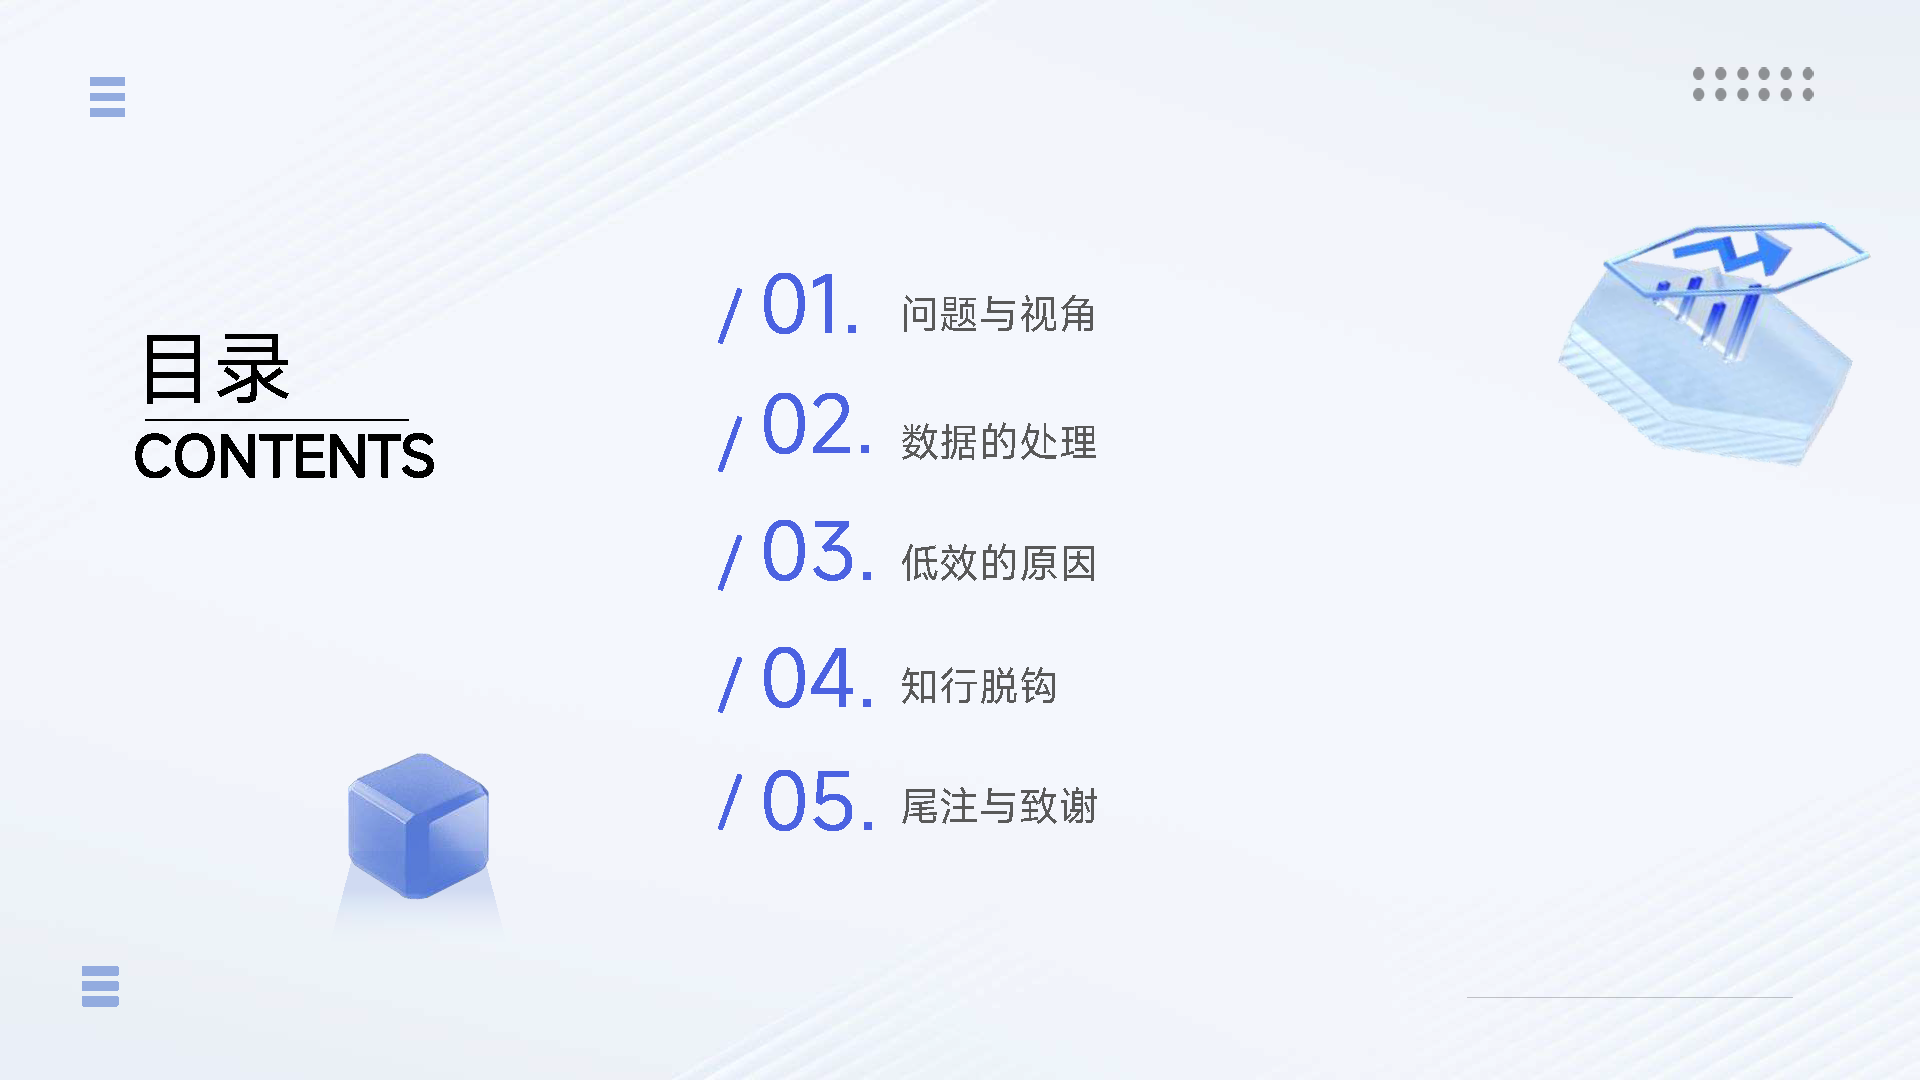
\includegraphics[width=\linewidth]{figure/image/image_页面_02.png}
\end{minipage}
\par\bigskip

\noindent
\begin{minipage}[t]{0.49\textwidth}
	\centering
	
\includegraphics[width=\linewidth]{figure/image/image_页面_03.png}
\end{minipage}\hfill
\begin{minipage}[t]{0.49\textwidth}
	\centering
	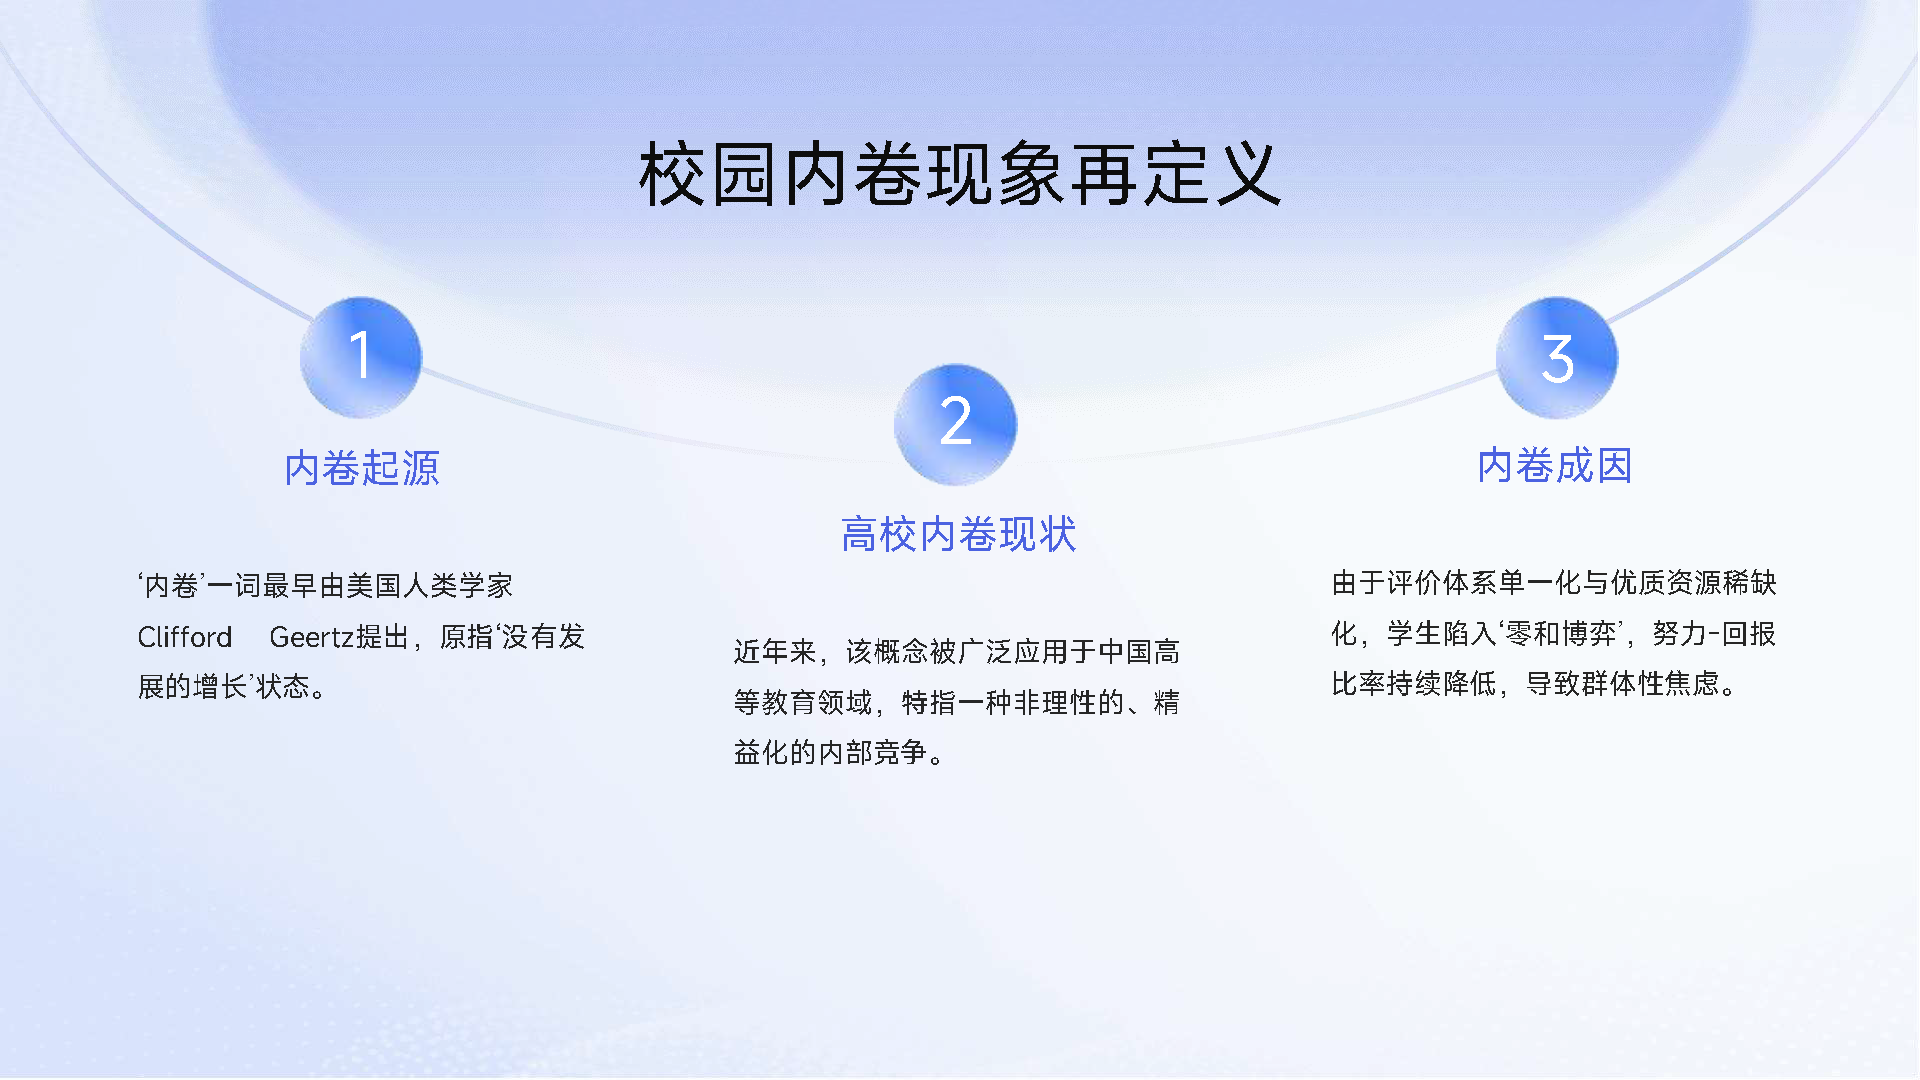
\includegraphics[width=\linewidth]{figure/image/image_页面_04.png}
\end{minipage}
\par\bigskip

\noindent
\begin{minipage}[t]{0.49\textwidth}
	\centering
	
\includegraphics[width=\linewidth]{figure/image/image_页面_05.png}
\end{minipage}\hfill
\begin{minipage}[t]{0.49\textwidth}
	\centering
	
\includegraphics[width=\linewidth]{figure/image/image_页面_06.png}
\end{minipage}
\par\bigskip

\noindent
\begin{minipage}[t]{0.49\textwidth}
	\centering
	
\includegraphics[width=\linewidth]{figure/image/image_页面_07.png}
\end{minipage}\hfill
\begin{minipage}[t]{0.49\textwidth}
	\centering
	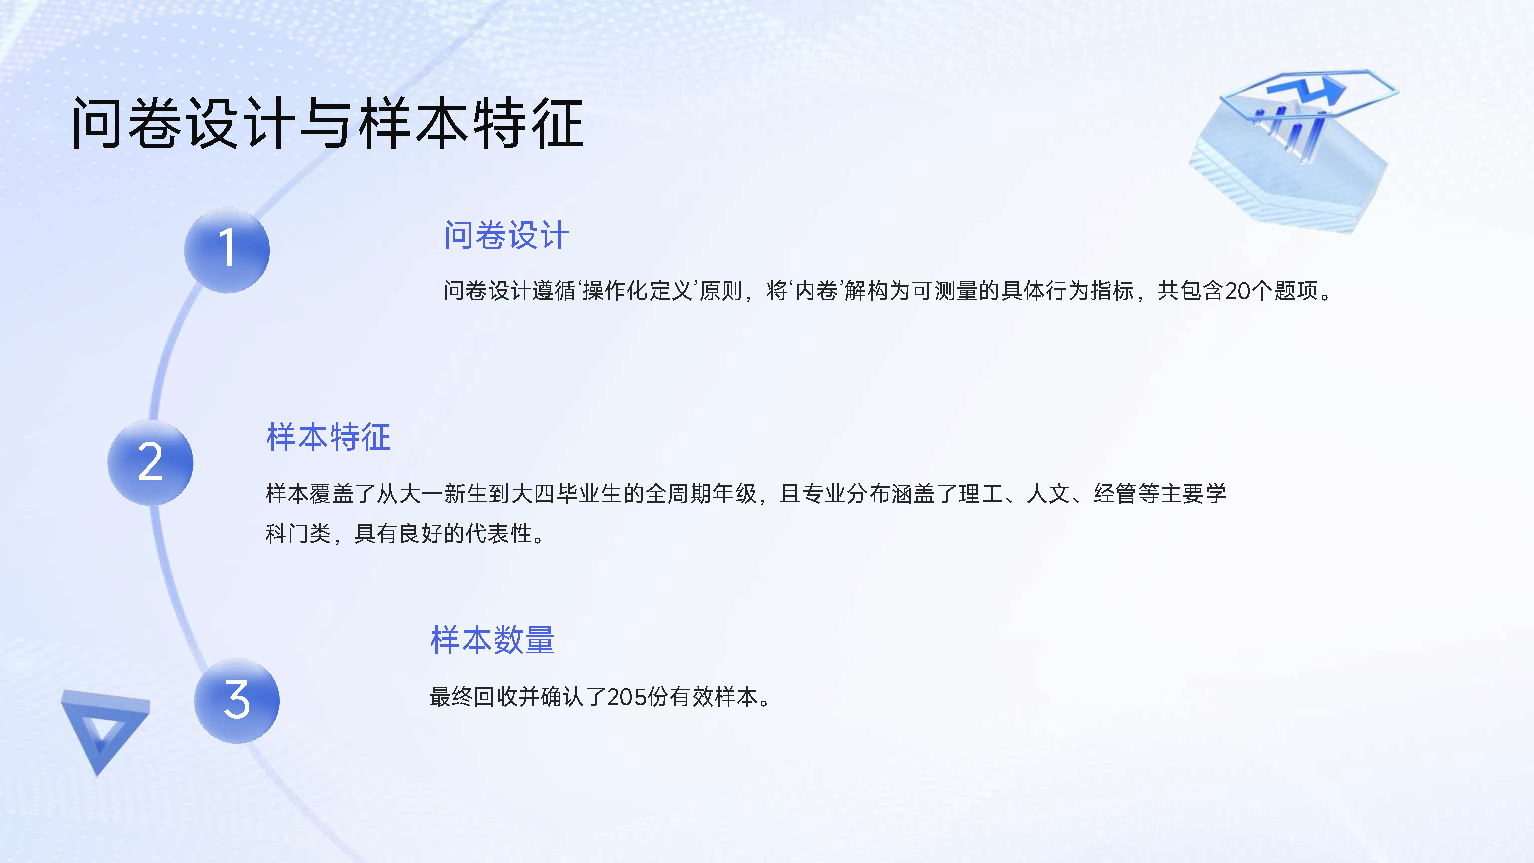
\includegraphics[width=\linewidth]{figure/image/image_页面_08.png}
\end{minipage}
\par\bigskip

\noindent
\begin{minipage}[t]{0.49\textwidth}
	\centering
	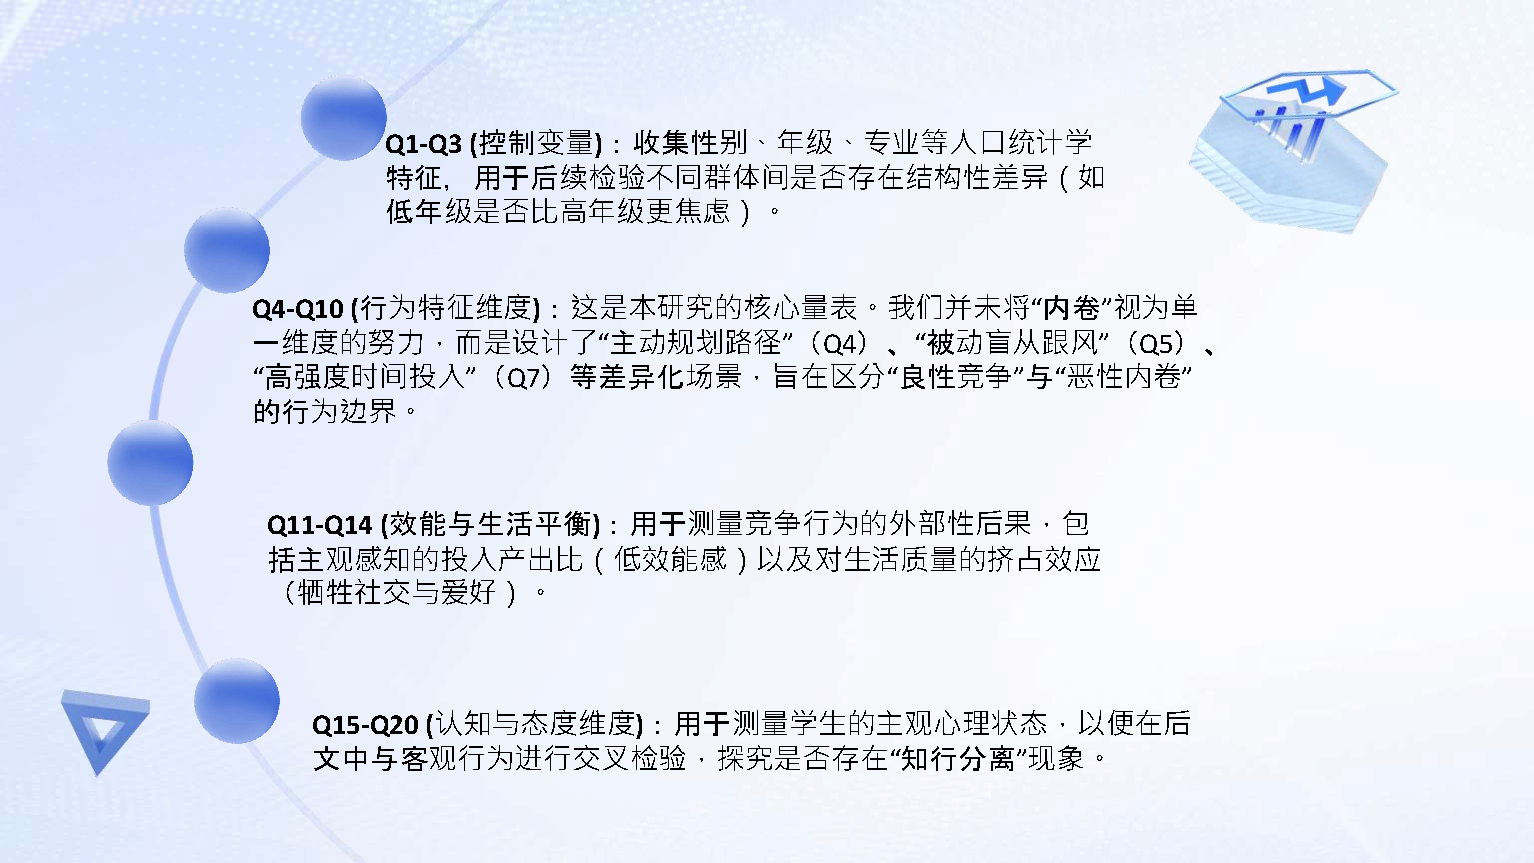
\includegraphics[width=\linewidth]{figure/image/image_页面_09.png}
\end{minipage}\hfill
\begin{minipage}[t]{0.49\textwidth}
	\centering
	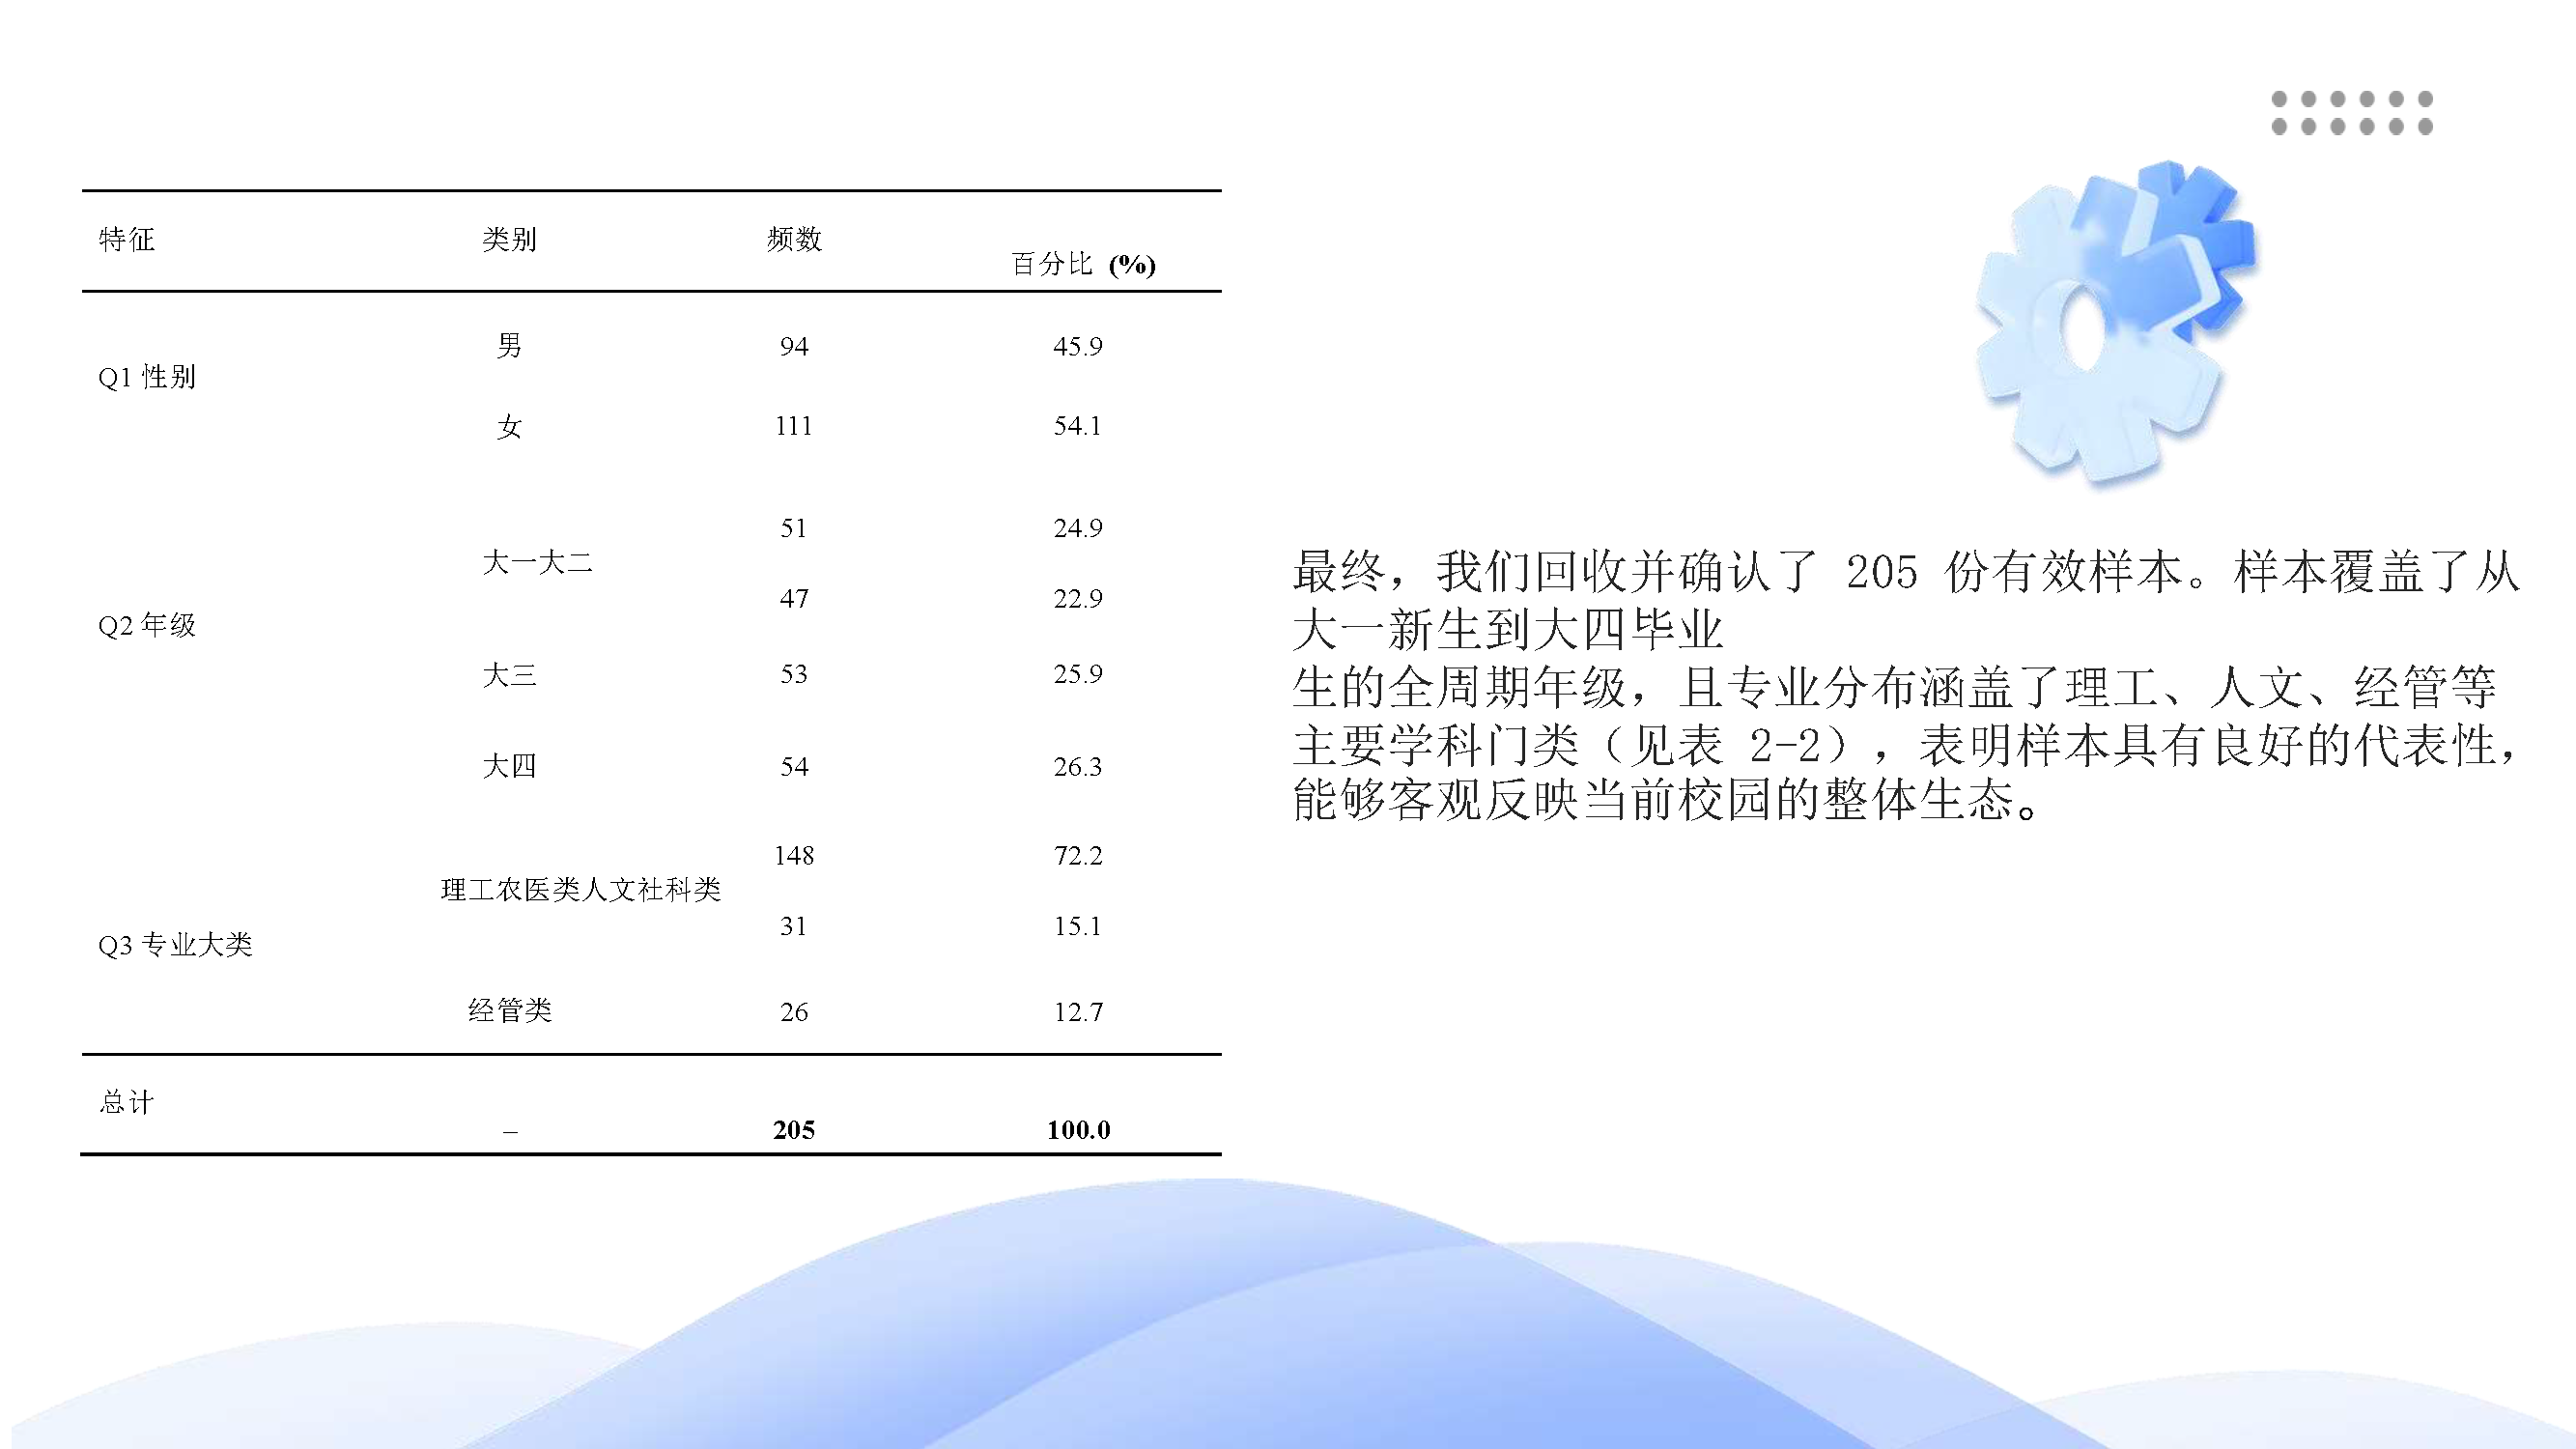
\includegraphics[width=\linewidth]{figure/image/image_页面_10.png}
\end{minipage}
\par\bigskip

\noindent
\begin{minipage}[t]{0.49\textwidth}
	\centering
	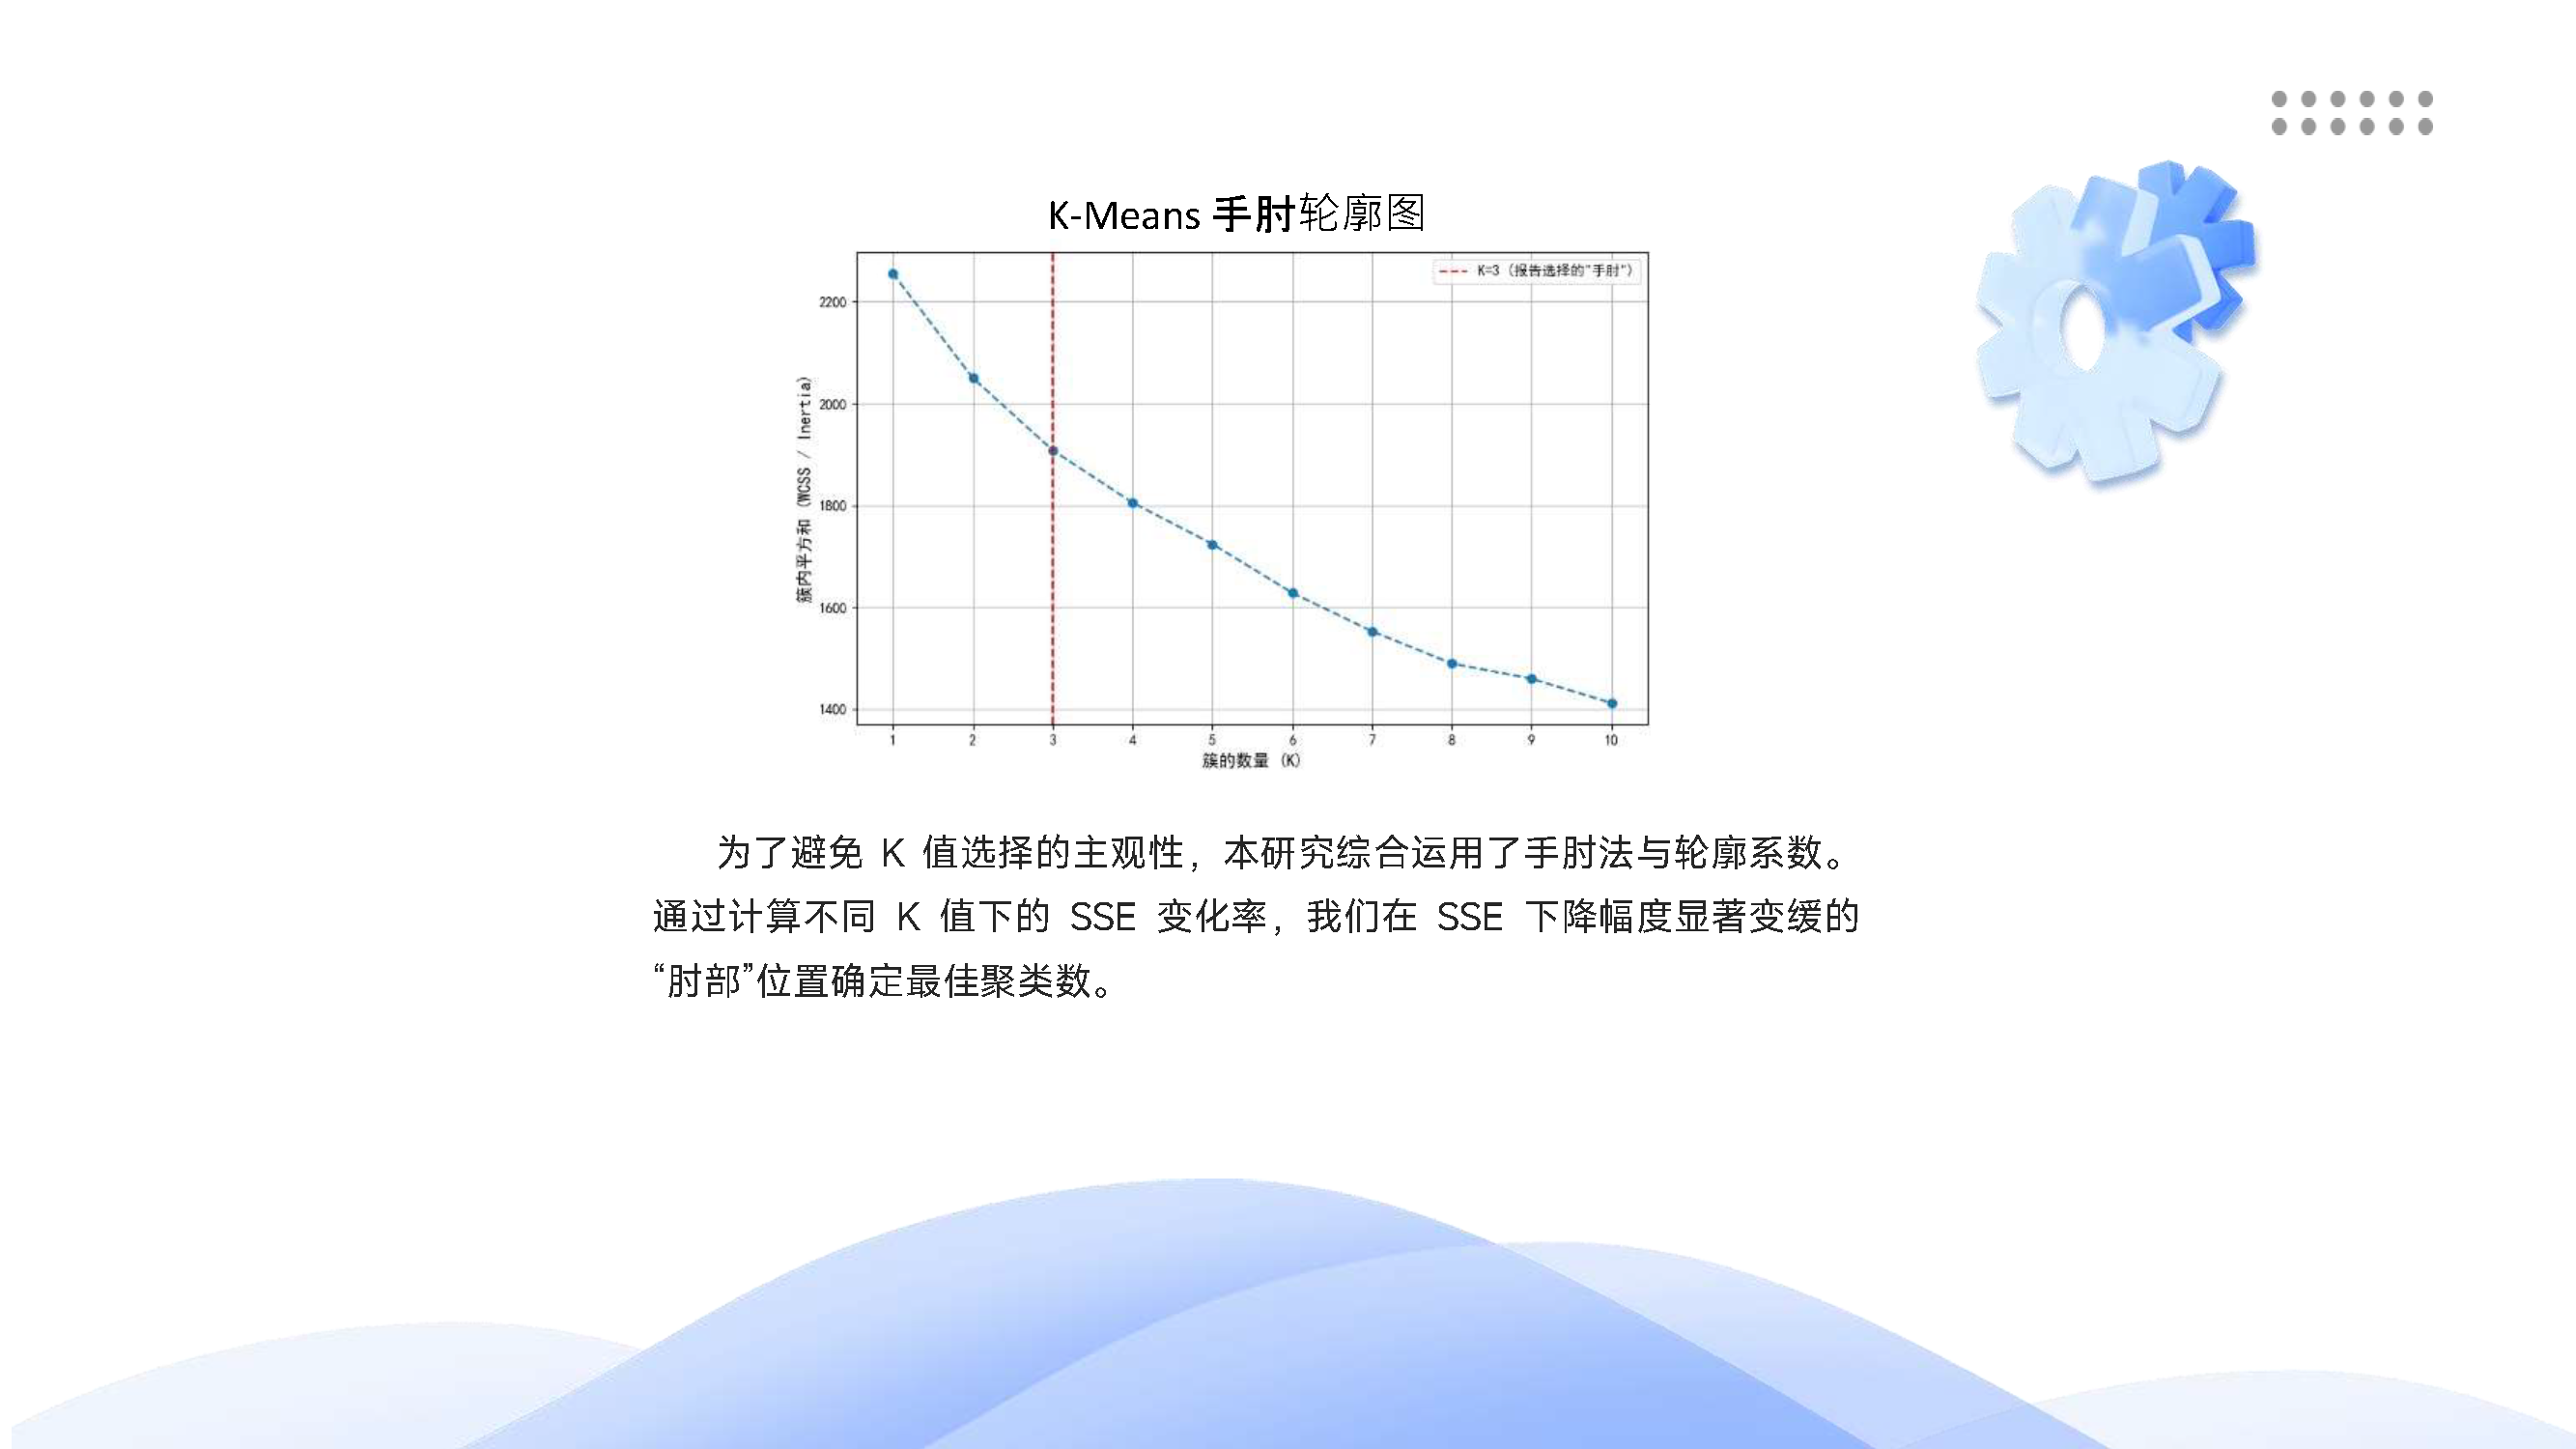
\includegraphics[width=\linewidth]{figure/image/image_页面_11.png}
\end{minipage}\hfill
\begin{minipage}[t]{0.49\textwidth}
	\centering
	
\includegraphics[width=\linewidth]{figure/image/image_页面_12.png}
\end{minipage}
\par\bigskip

\noindent
\begin{minipage}[t]{0.49\textwidth}
	\centering
	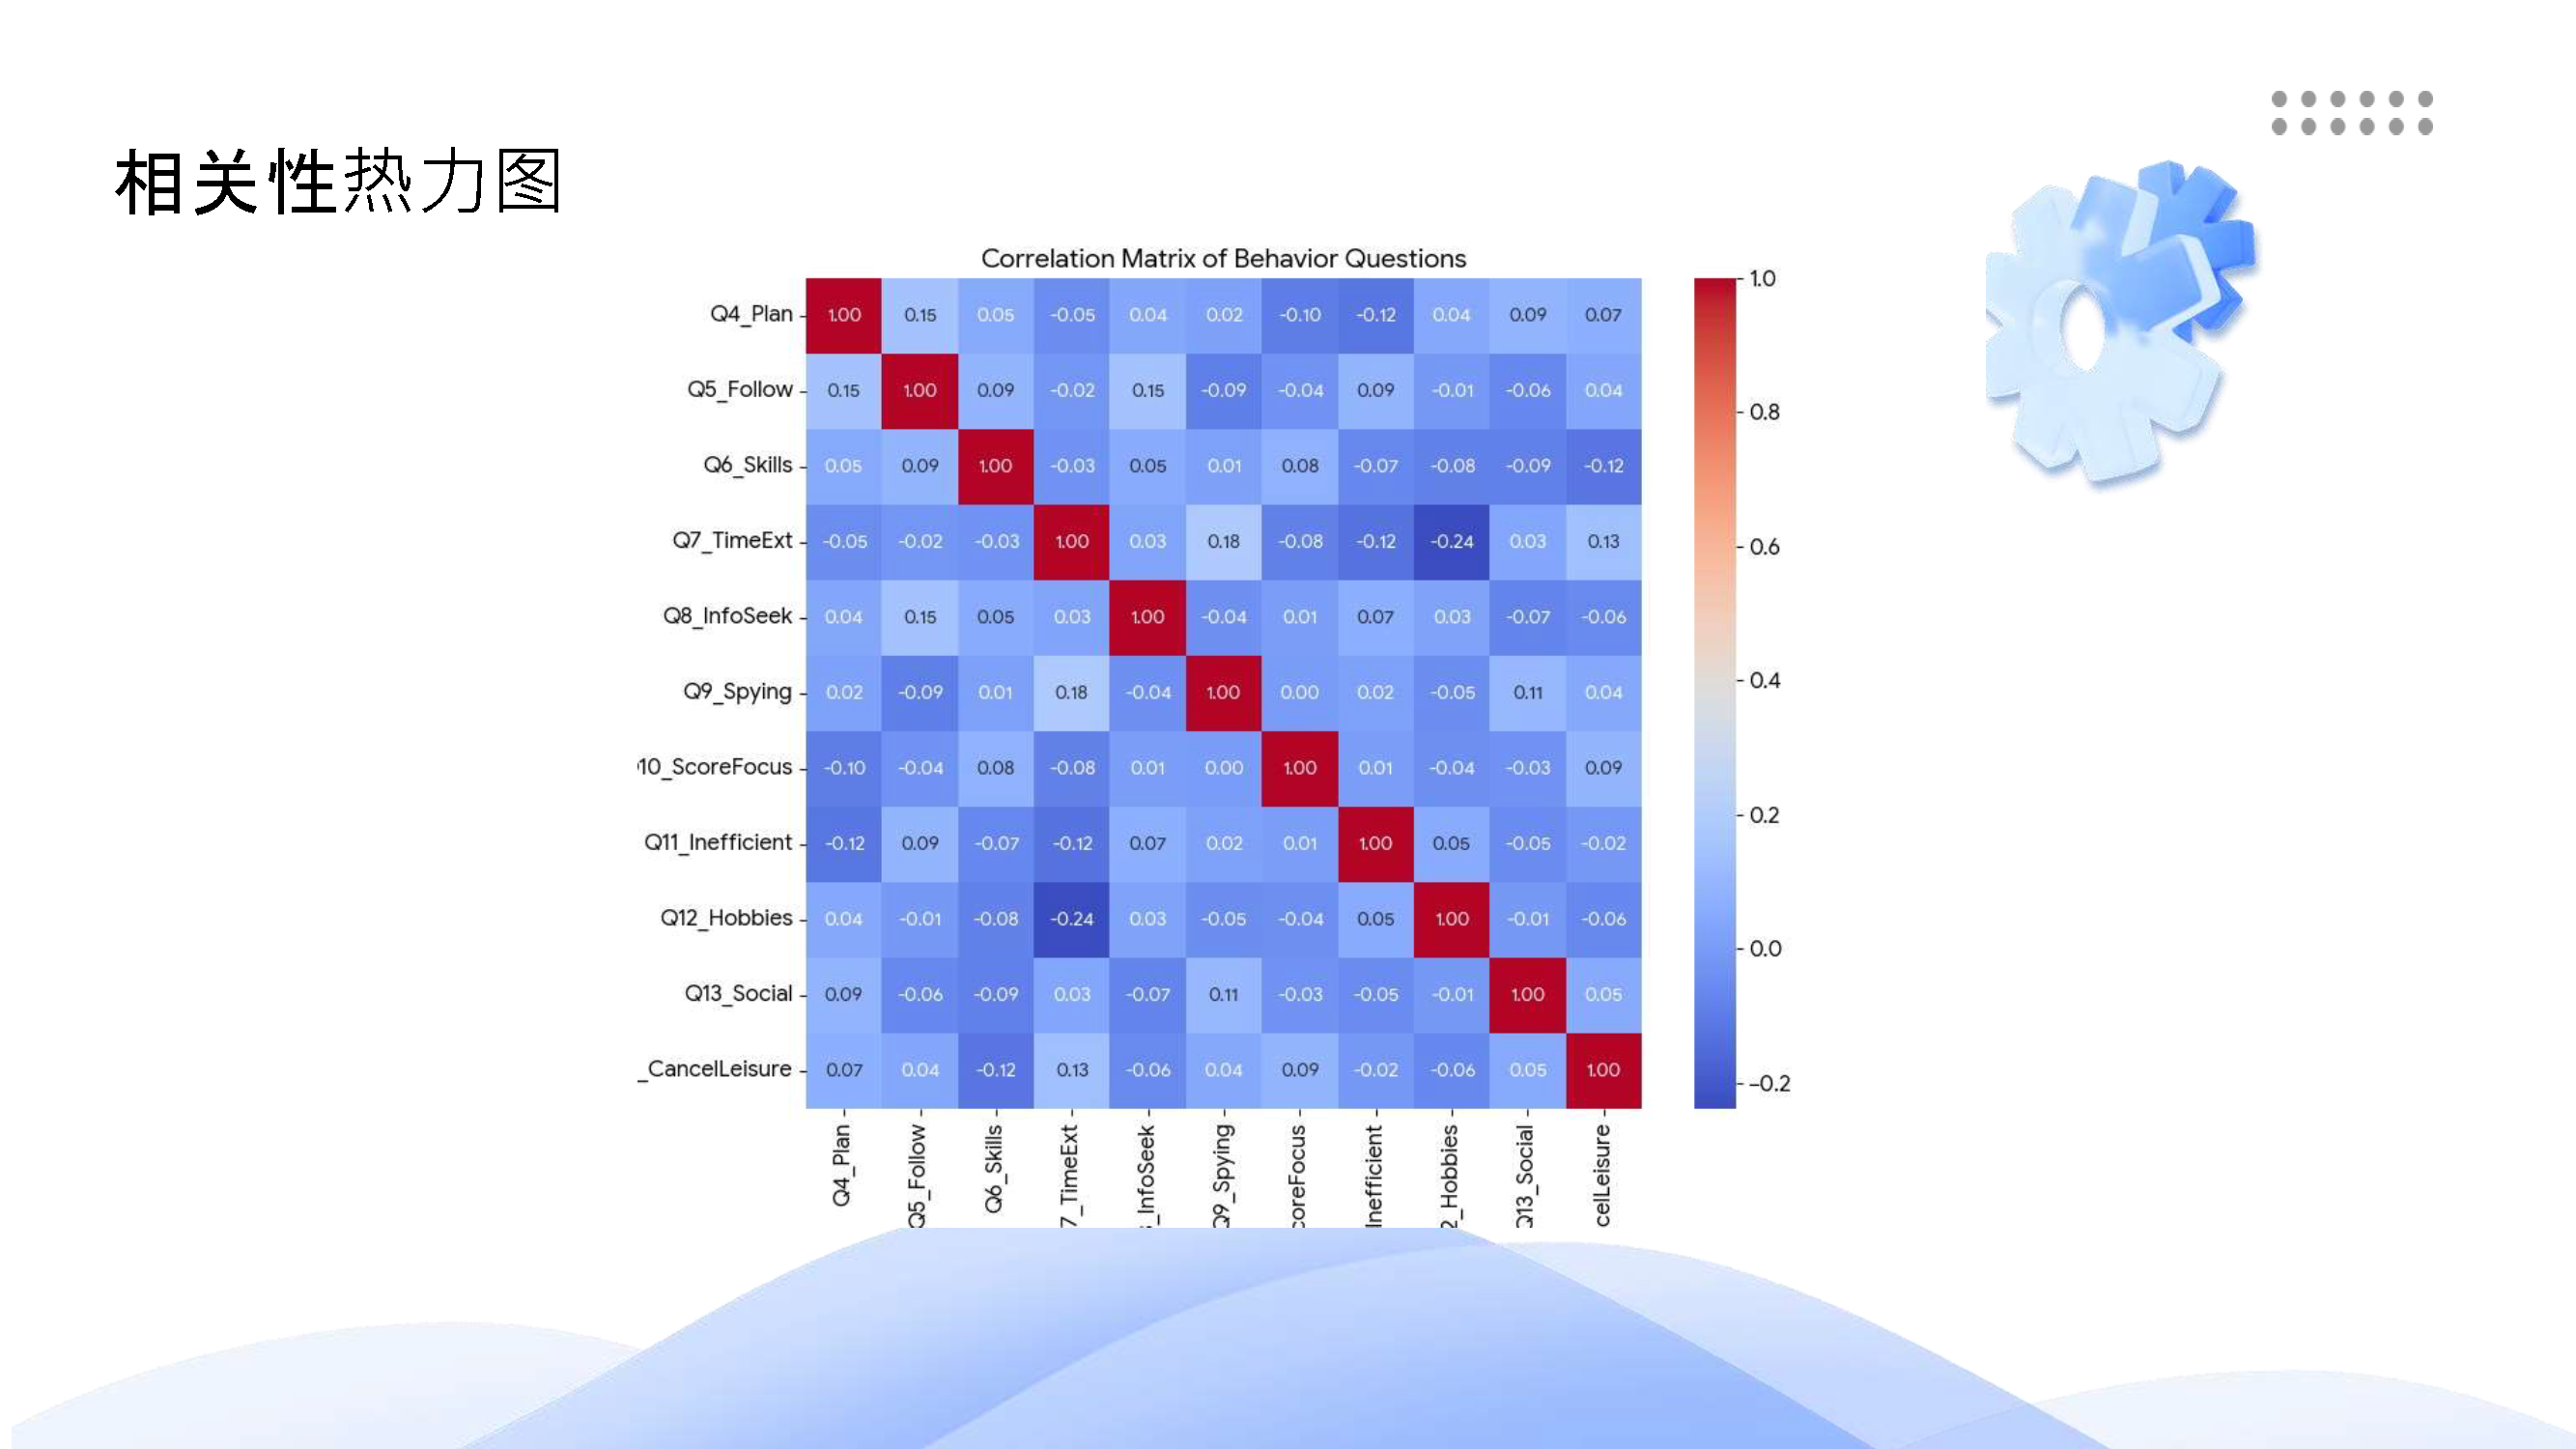
\includegraphics[width=\linewidth]{figure/image/image_页面_13.png}
\end{minipage}\hfill
\begin{minipage}[t]{0.49\textwidth}
	\centering
	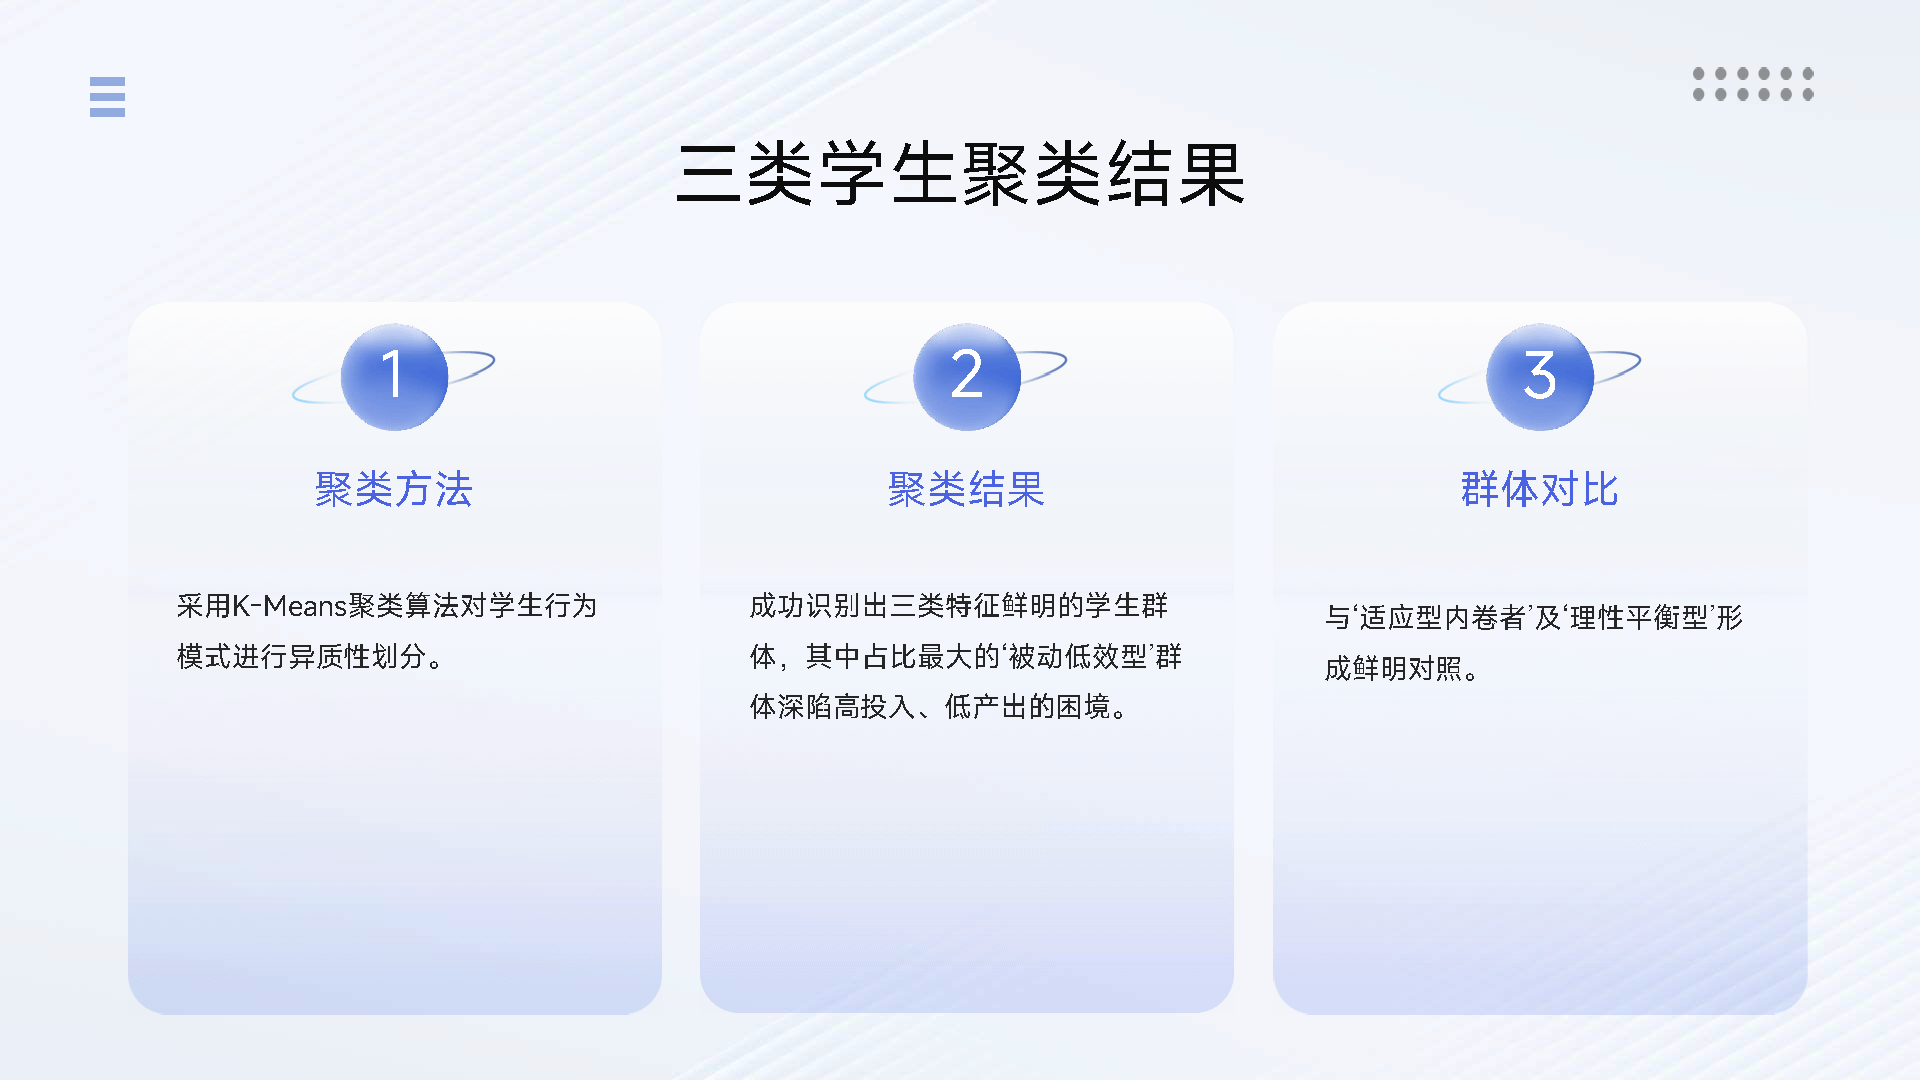
\includegraphics[width=\linewidth]{figure/image/image_页面_14.png}
\end{minipage}
\par\bigskip

\noindent
\begin{minipage}[t]{0.49\textwidth}
	\centering
	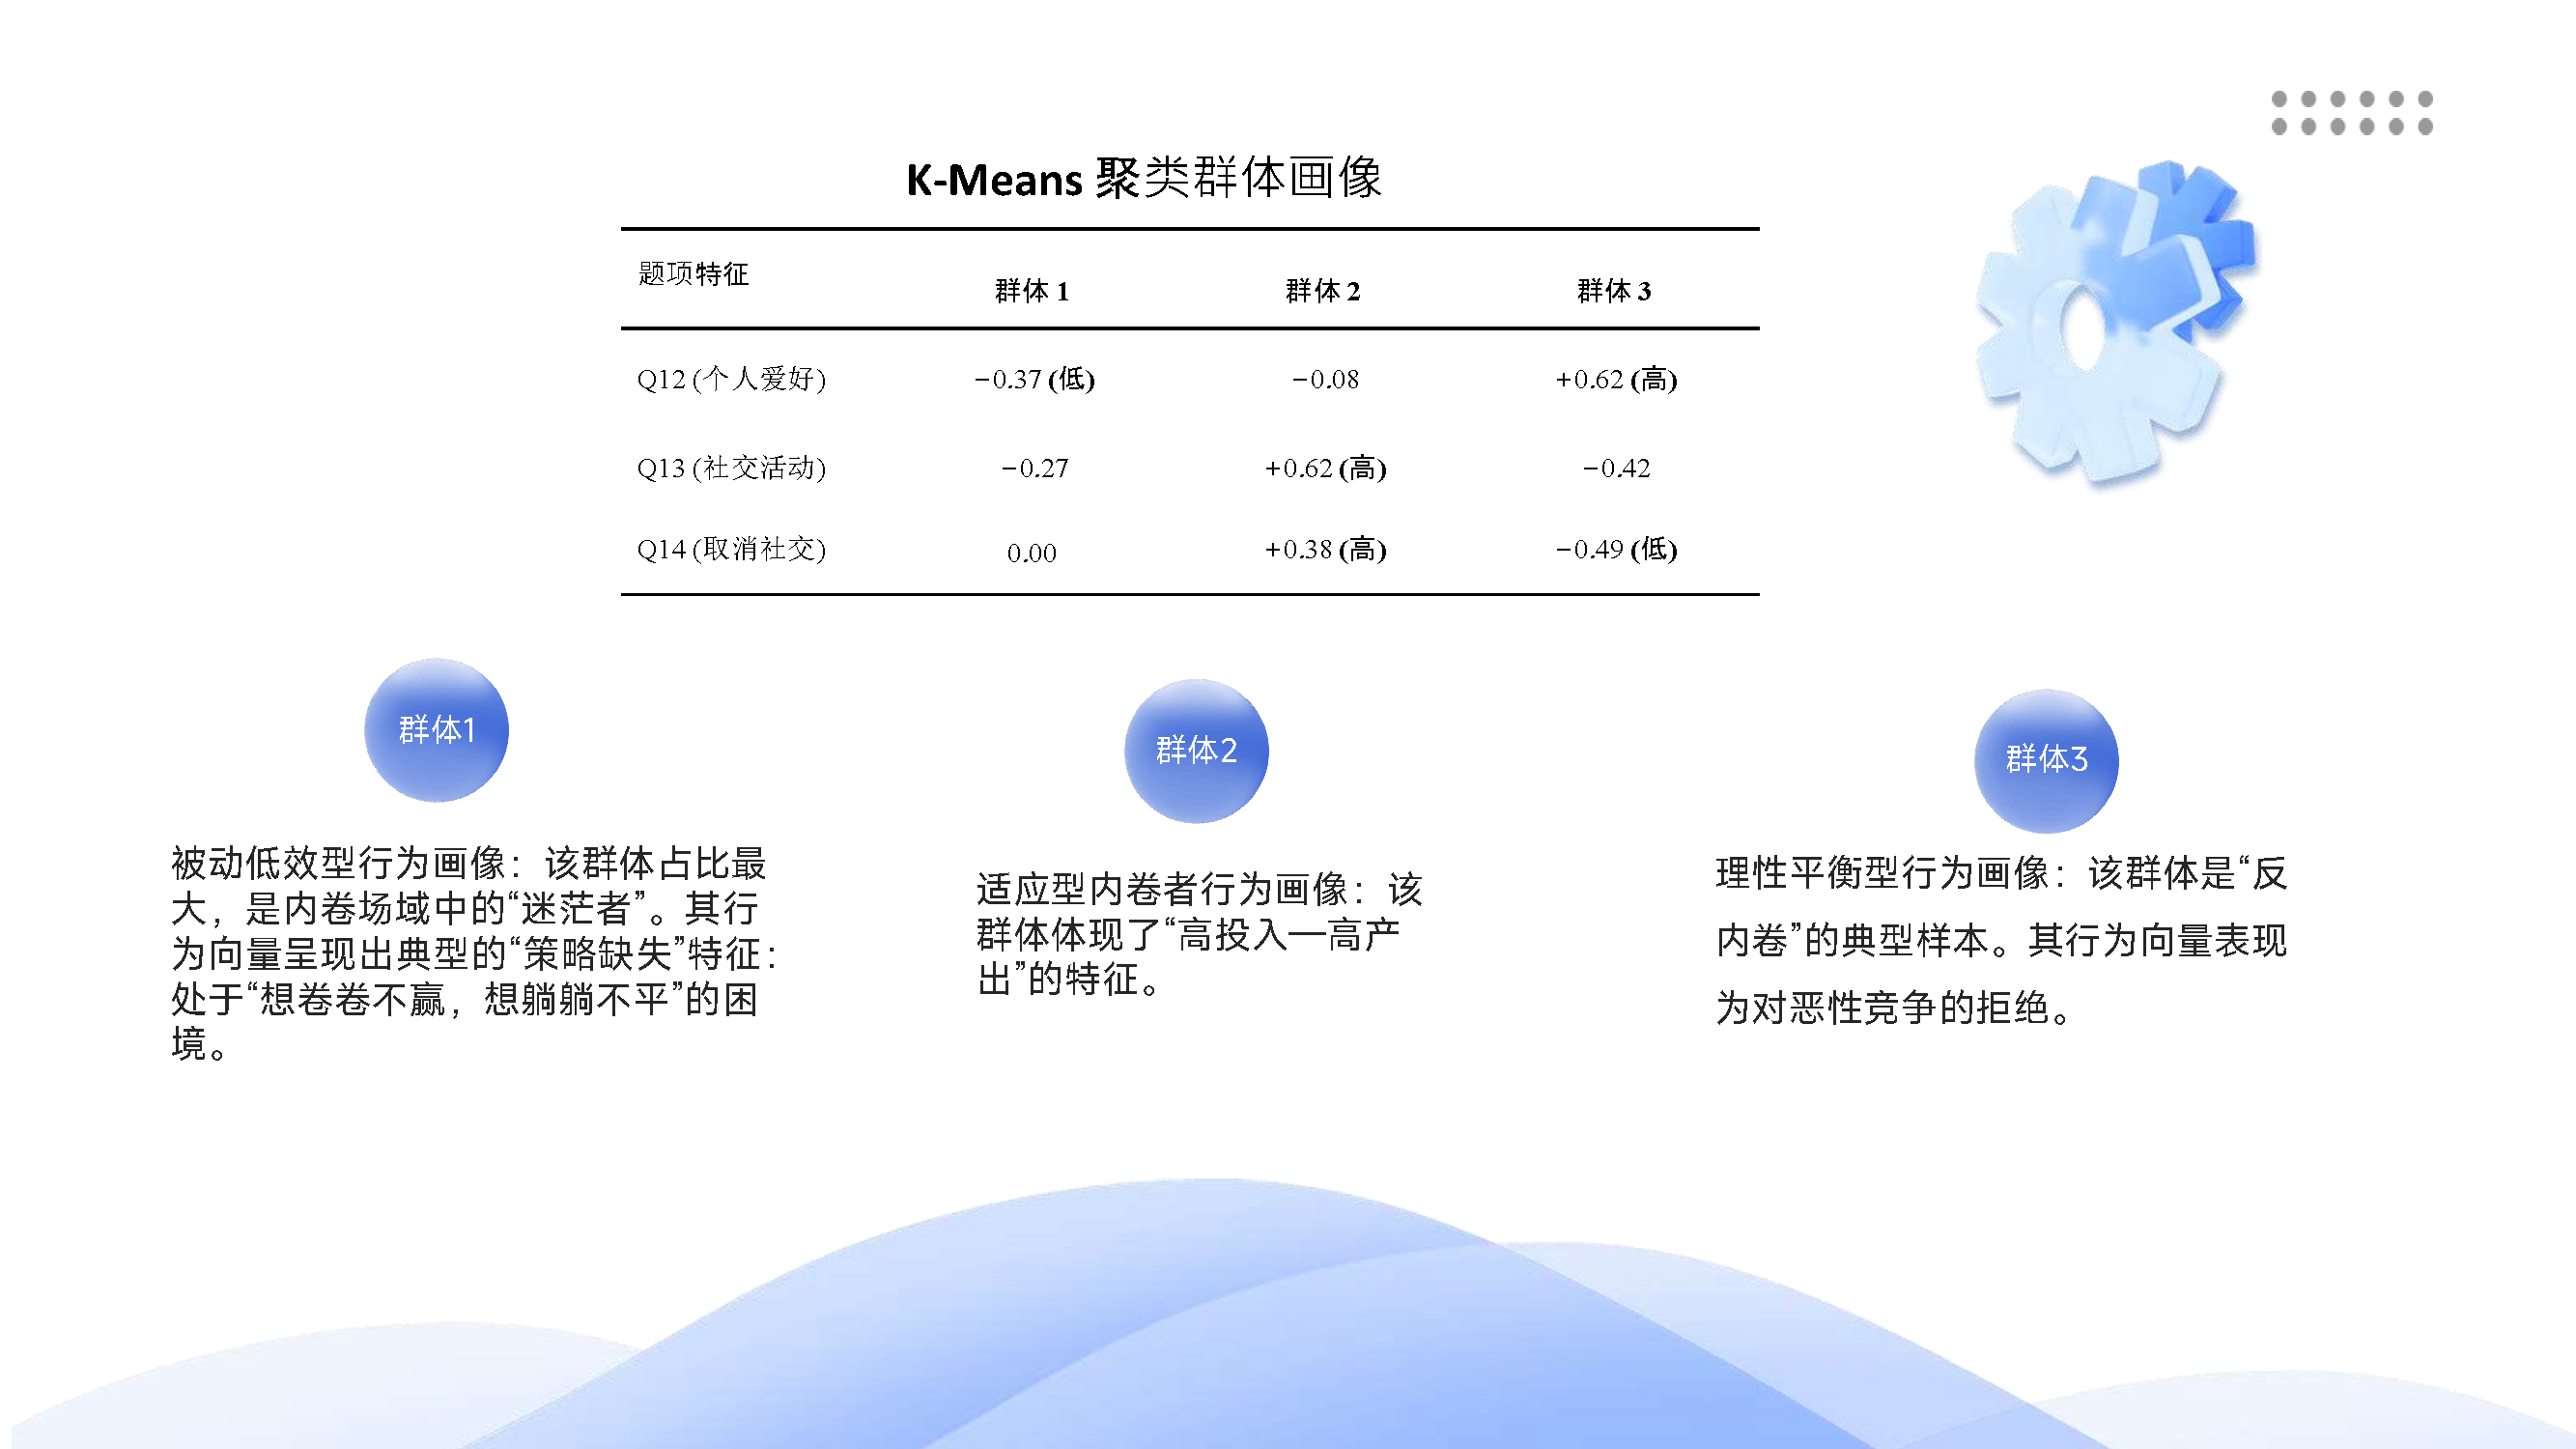
\includegraphics[width=\linewidth]{figure/image/image_页面_15.png}
\end{minipage}\hfill
\begin{minipage}[t]{0.49\textwidth}
	\centering
	
\includegraphics[width=\linewidth]{figure/image/image_页面_16.png}
\end{minipage}
\par\bigskip

\noindent
\begin{minipage}[t]{0.49\textwidth}
	\centering
	
\includegraphics[width=\linewidth]{figure/image/image_页面_17.png}
\end{minipage}\hfill
\begin{minipage}[t]{0.49\textwidth}
	\centering
	
\includegraphics[width=\linewidth]{figure/image/image_页面_18.png}
\end{minipage}
\par\bigskip

\noindent
\begin{minipage}[t]{0.49\textwidth}
	\centering
	
\includegraphics[width=\linewidth]{figure/image/image_页面_19.png}
\end{minipage}\hfill
\begin{minipage}[t]{0.49\textwidth}
	\centering
	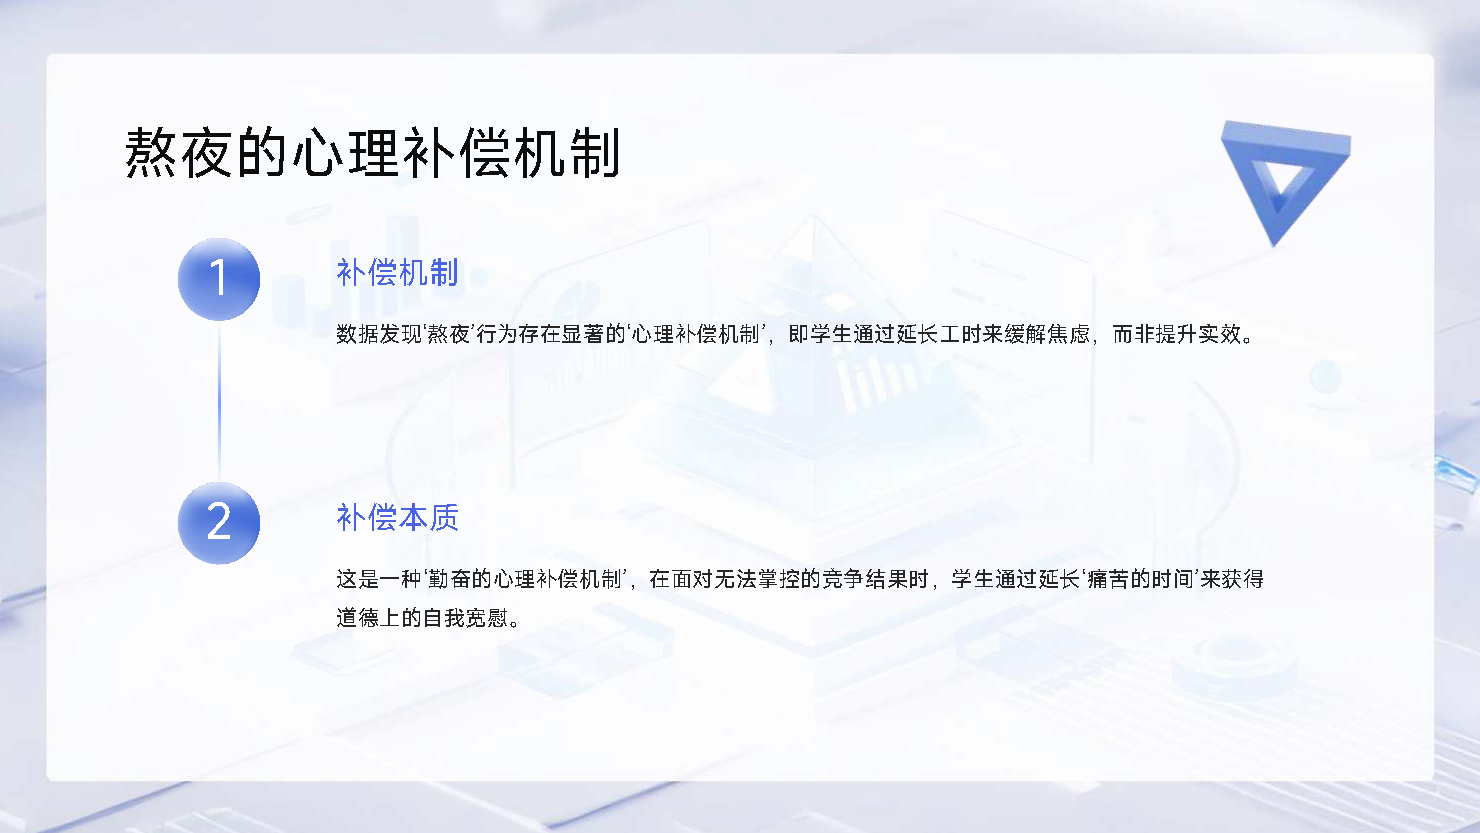
\includegraphics[width=\linewidth]{figure/image/image_页面_20.png}
\end{minipage}
\par\bigskip

\noindent
\begin{minipage}[t]{0.49\textwidth}
	\centering
	
\includegraphics[width=\linewidth]{figure/image/image_页面_21.png}
\end{minipage}\hfill
\begin{minipage}[t]{0.49\textwidth}
	\centering
	
\includegraphics[width=\linewidth]{figure/image/image_页面_22.png}
\end{minipage}
\par\bigskip

\noindent
\begin{minipage}[t]{0.49\textwidth}
	\centering
	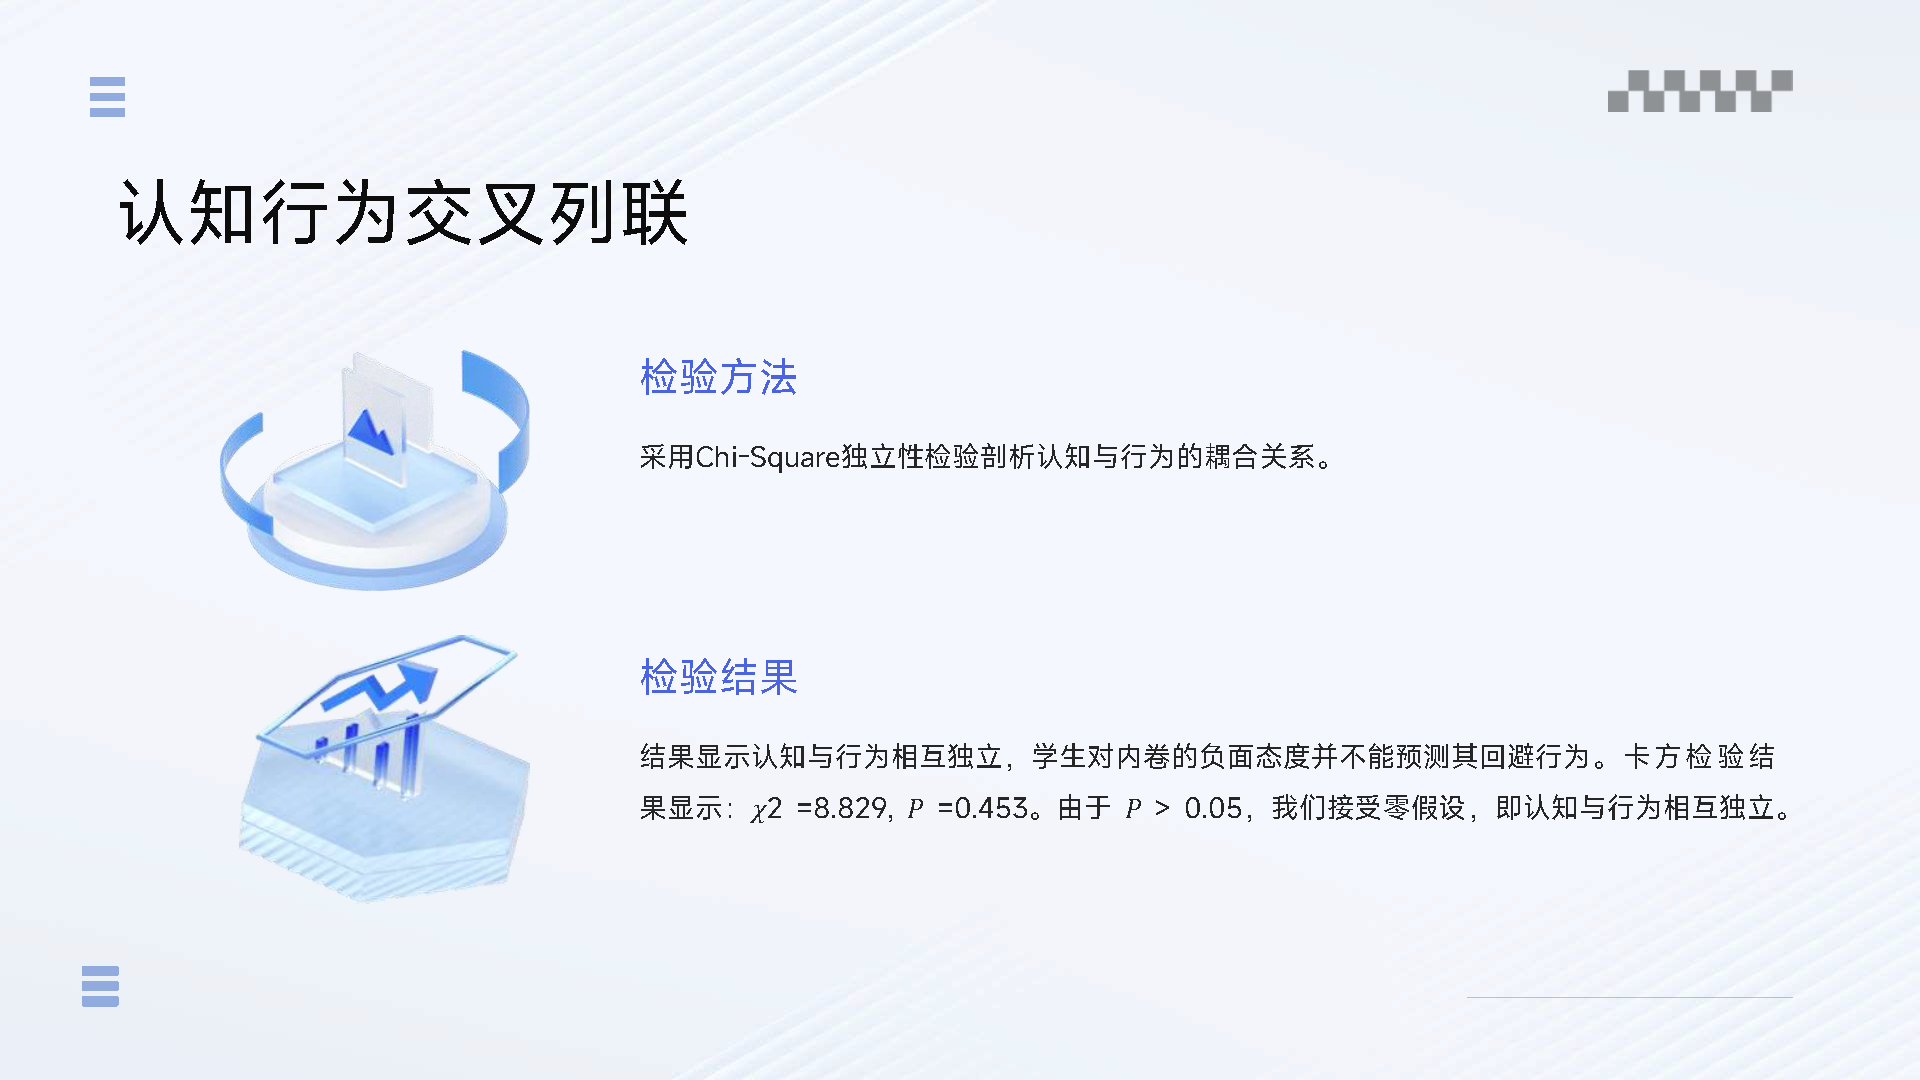
\includegraphics[width=\linewidth]{figure/image/image_页面_23.png}
\end{minipage}\hfill
\begin{minipage}[t]{0.49\textwidth}
	\centering
	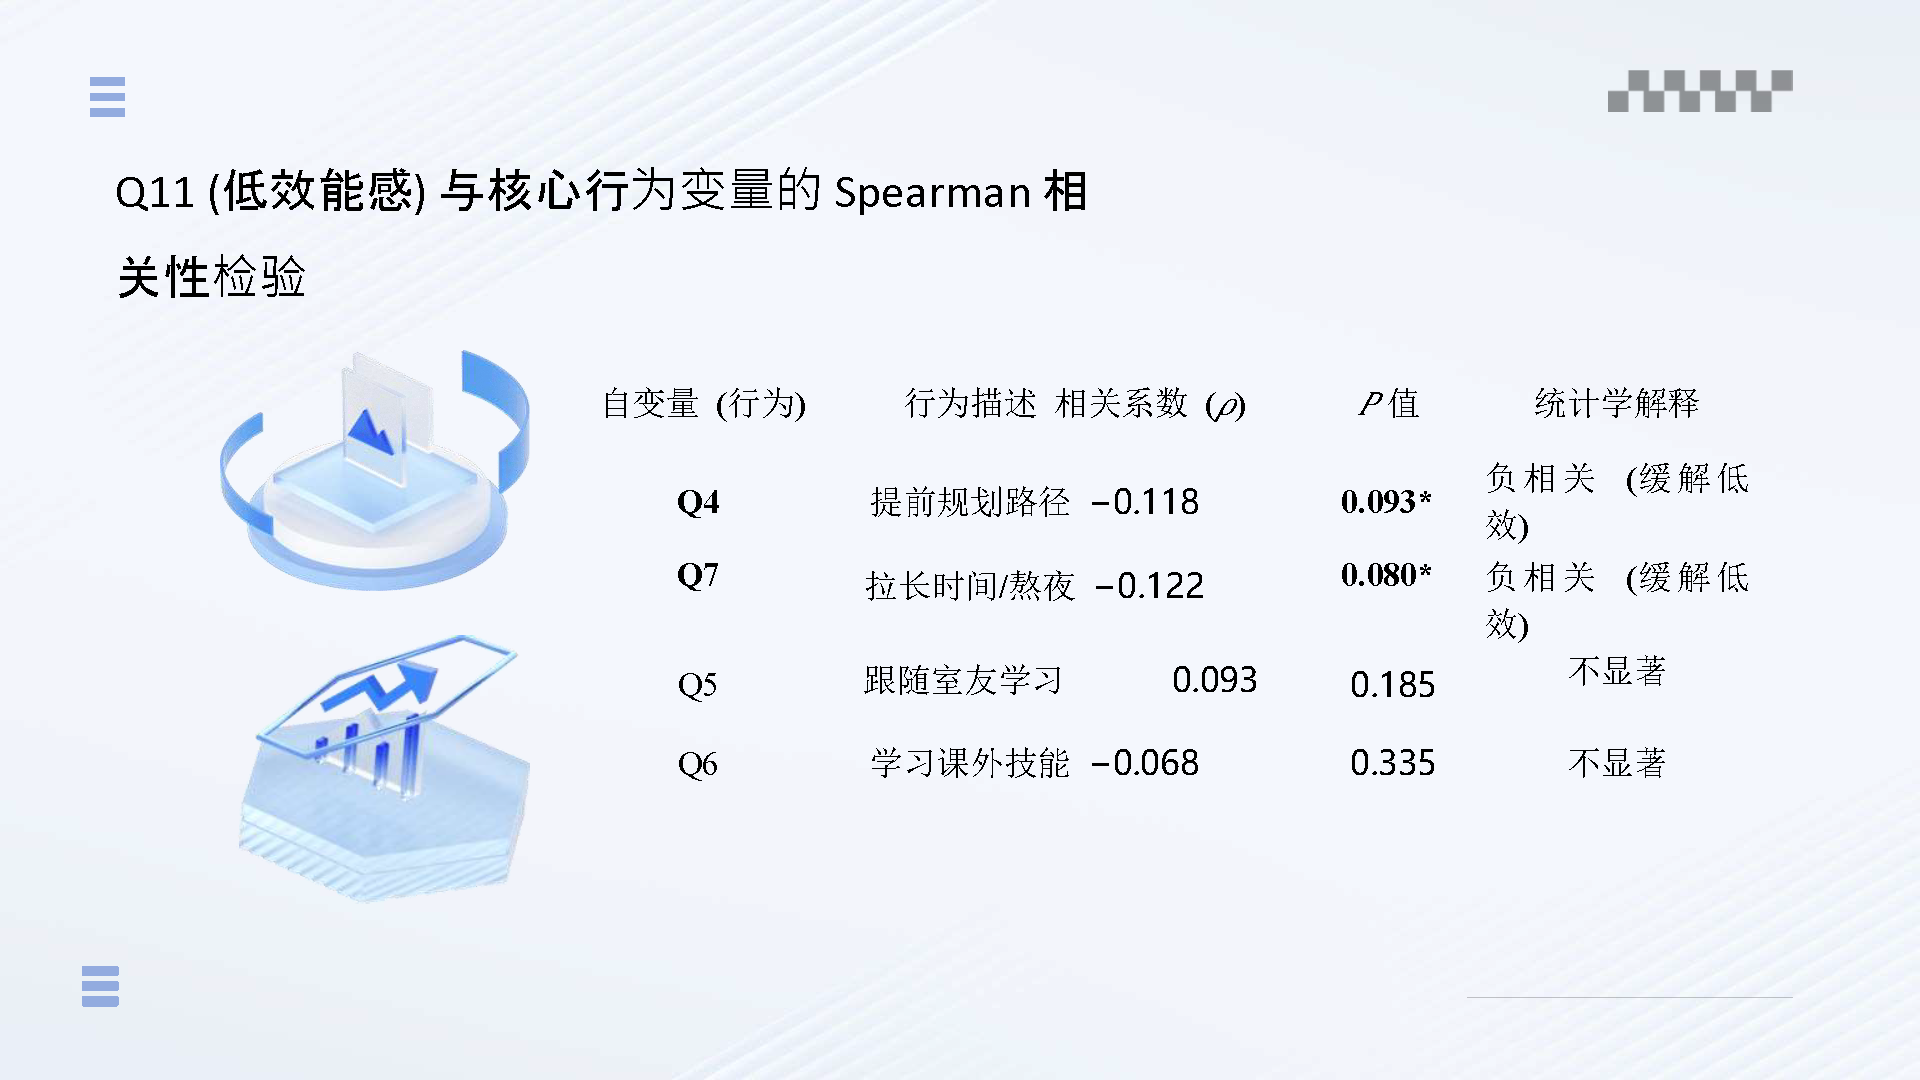
\includegraphics[width=\linewidth]{figure/image/image_页面_24.png}
\end{minipage}
\par\bigskip

\noindent
\begin{minipage}[t]{0.49\textwidth}
	\centering
	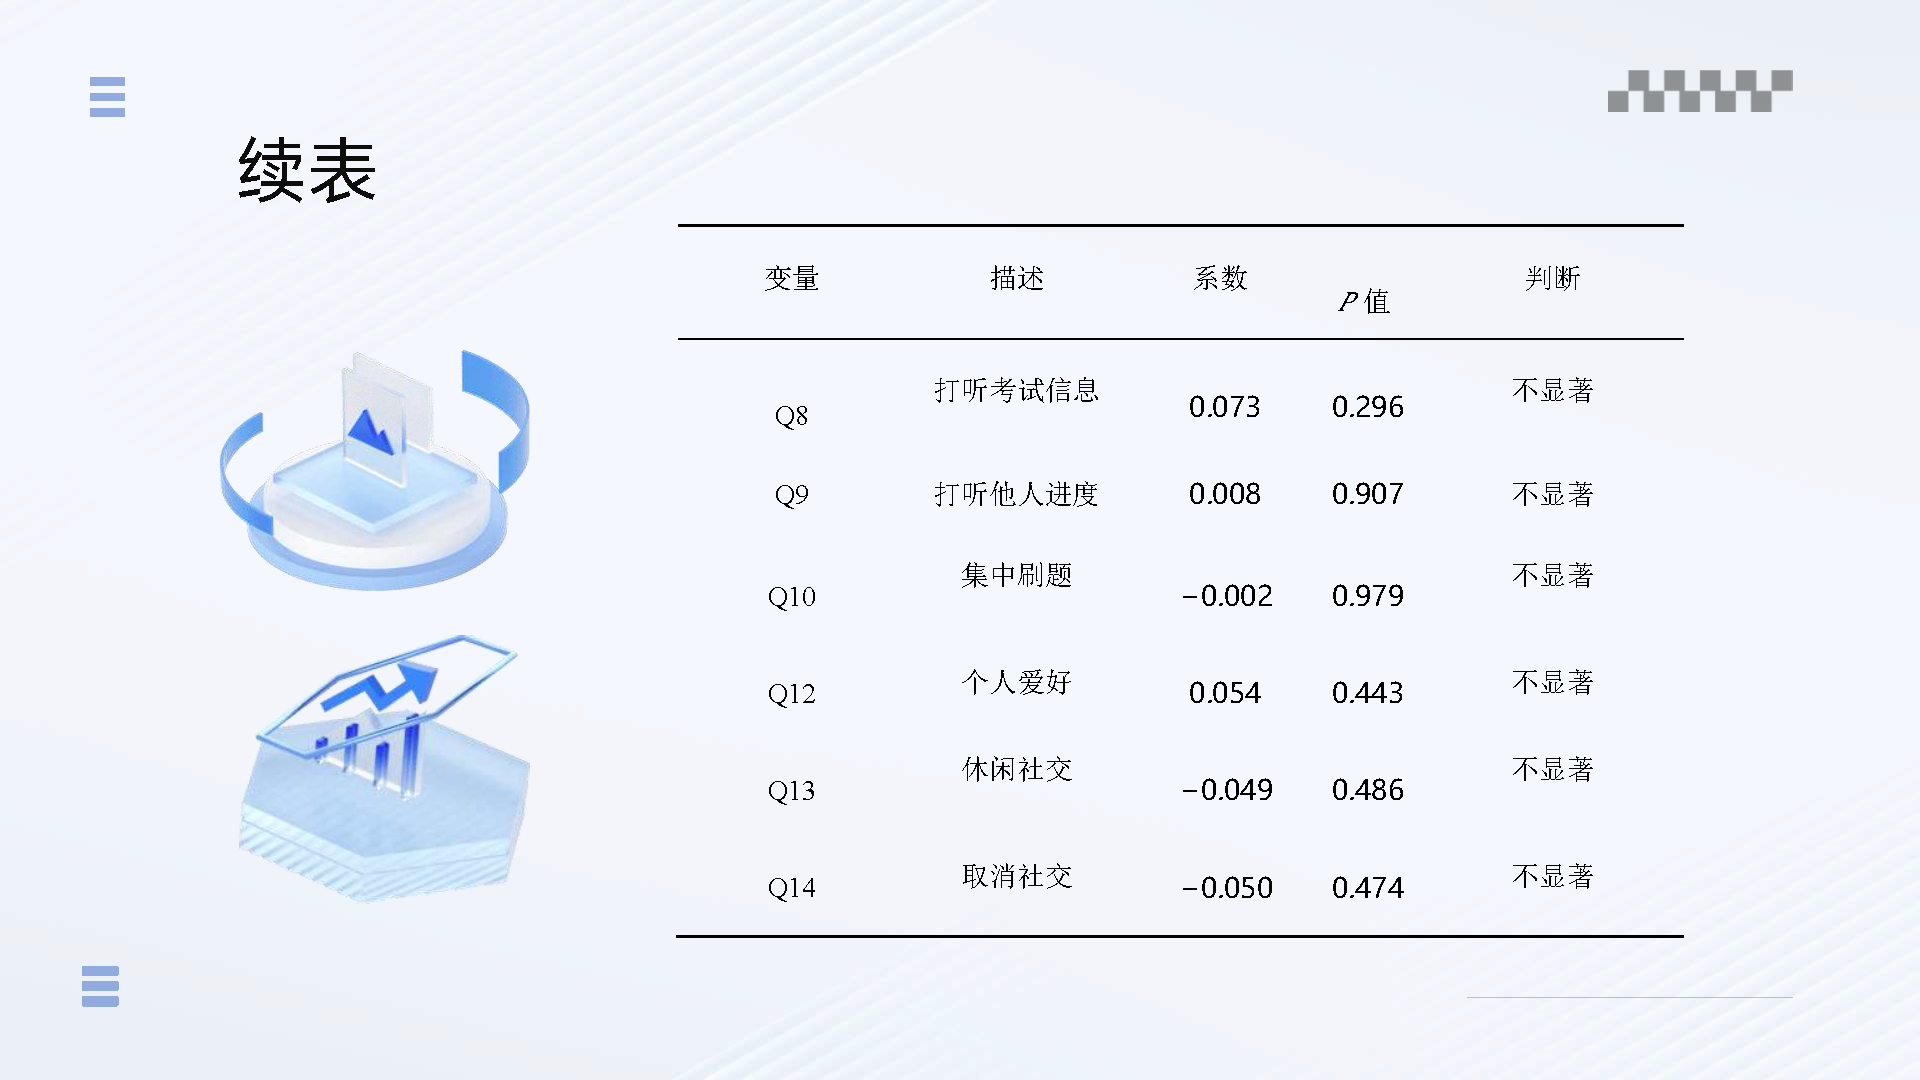
\includegraphics[width=\linewidth]{figure/image/image_页面_25.png}
\end{minipage}\hfill
\begin{minipage}[t]{0.49\textwidth}
	\centering
	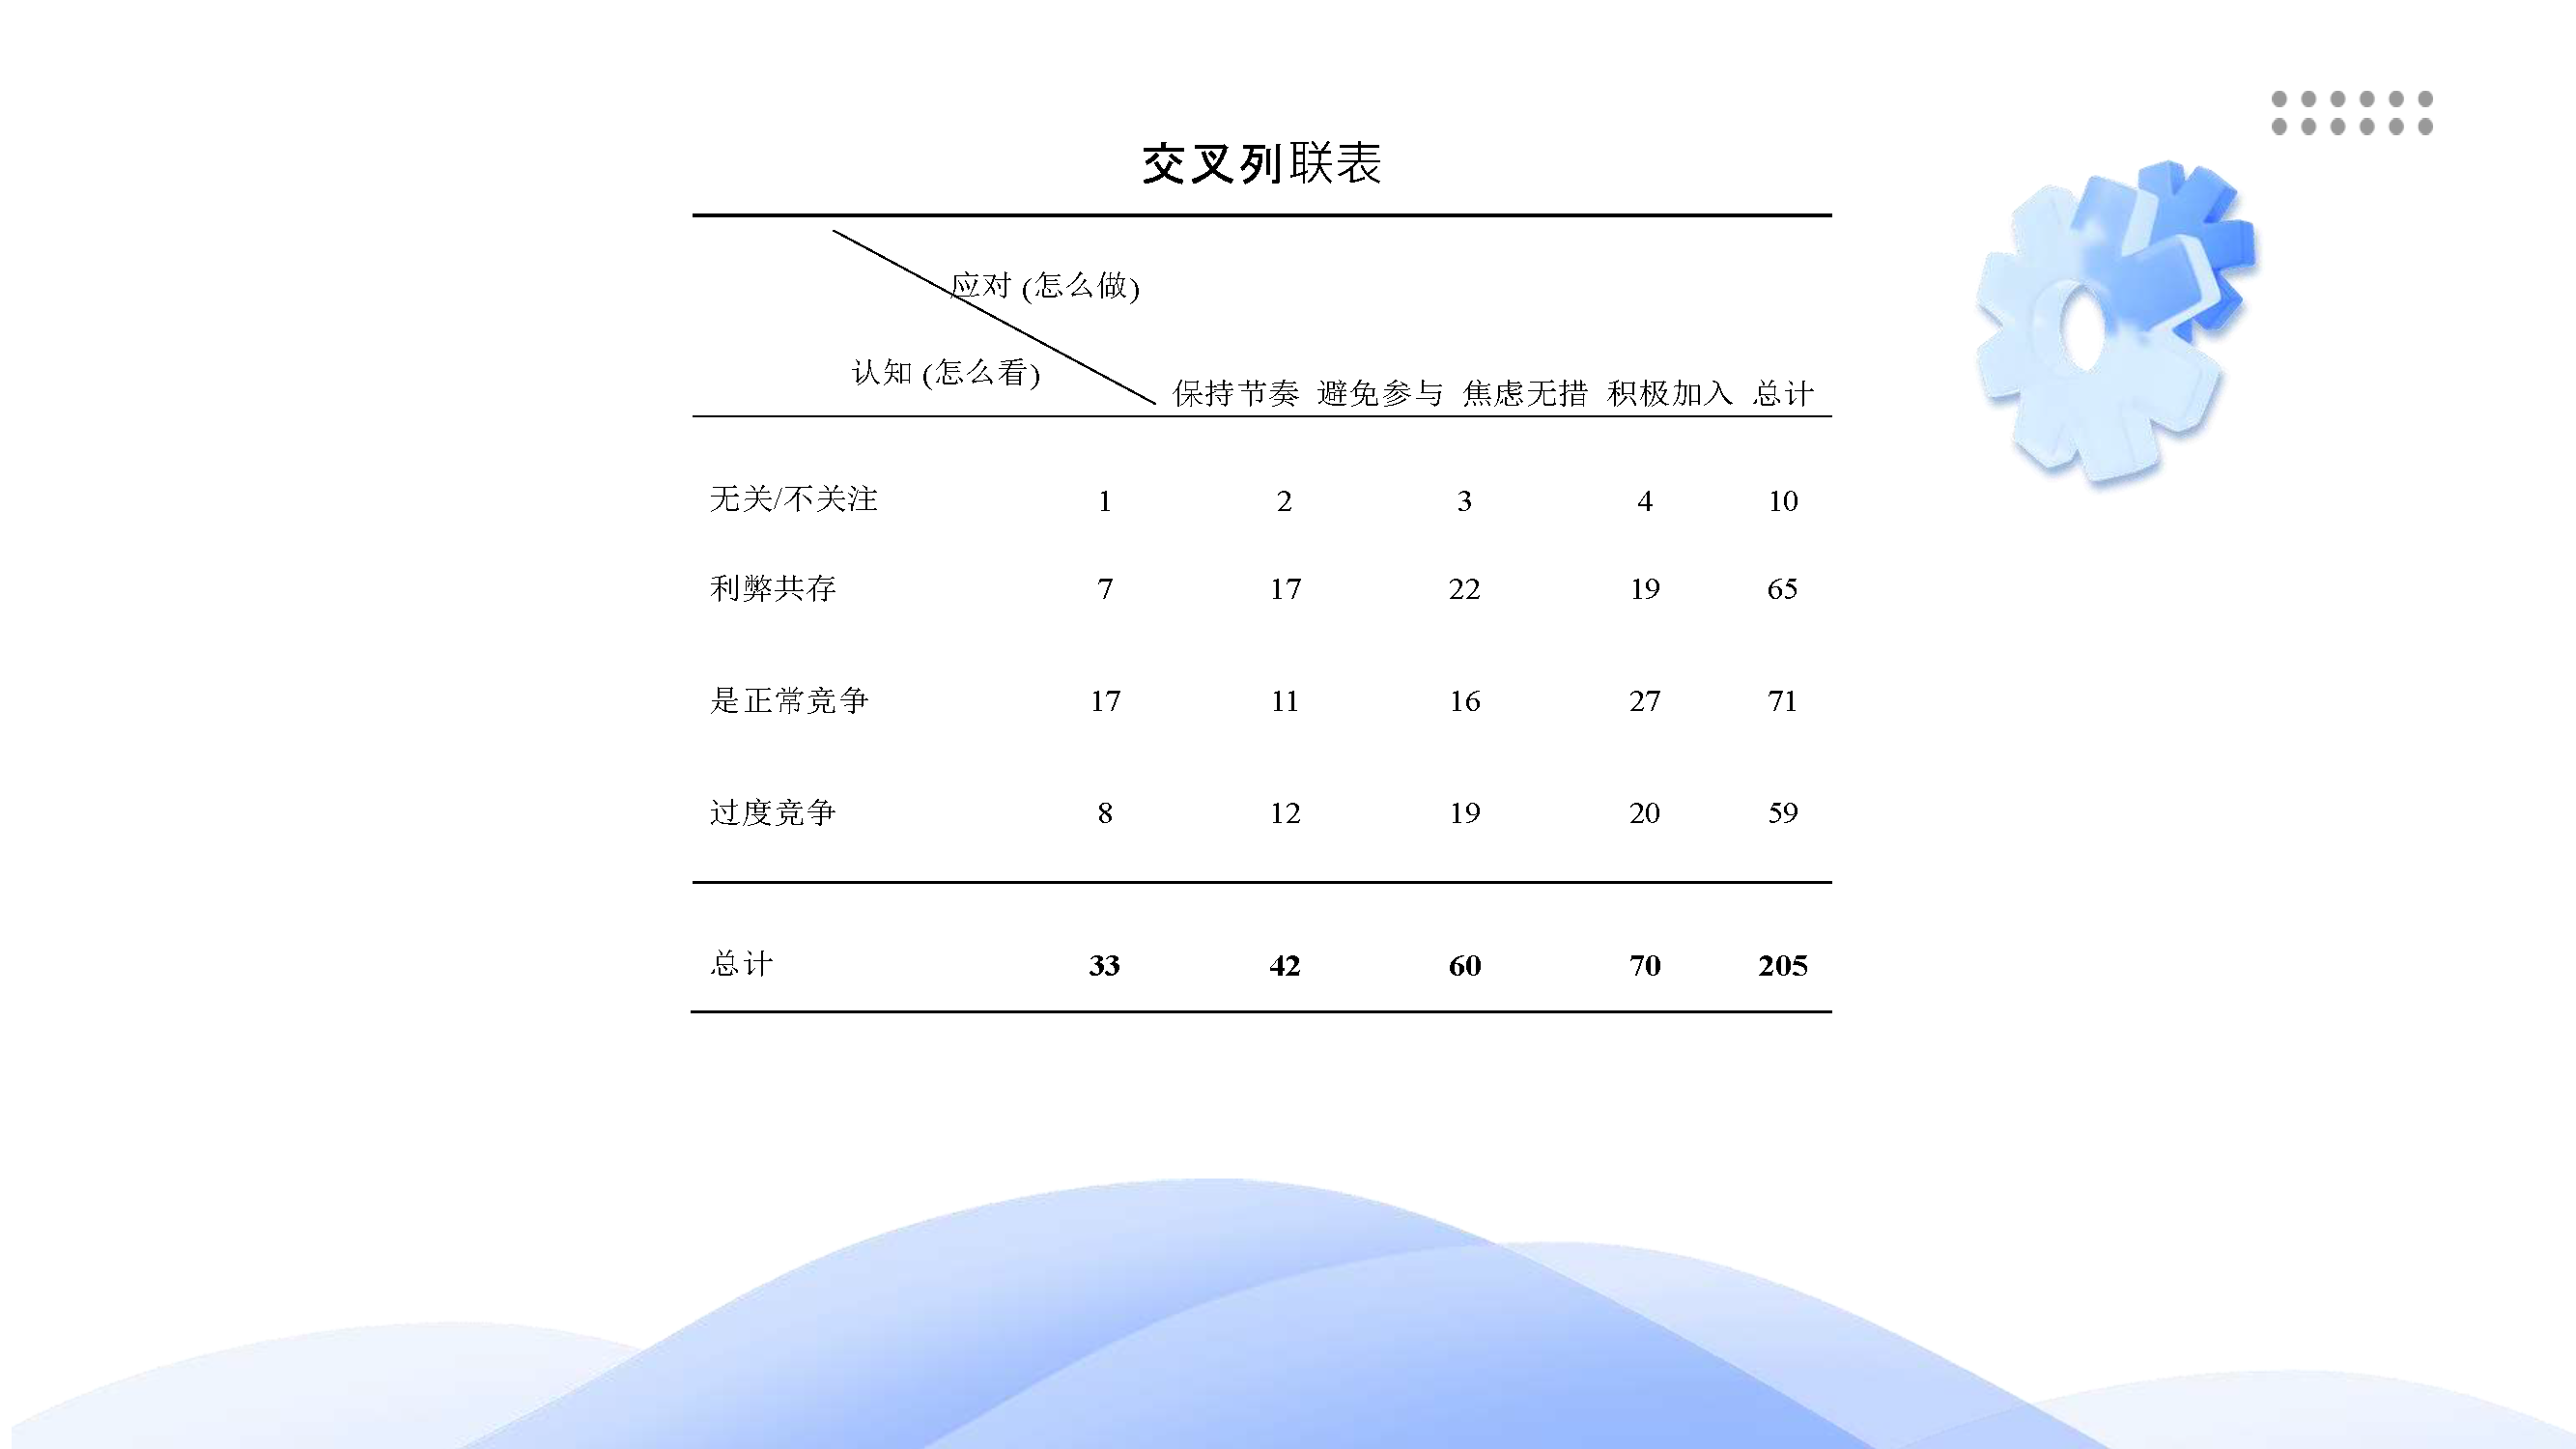
\includegraphics[width=\linewidth]{figure/image/image_页面_26.png}
\end{minipage}
\par\bigskip

\noindent
\begin{minipage}[t]{0.49\textwidth}
	\centering
	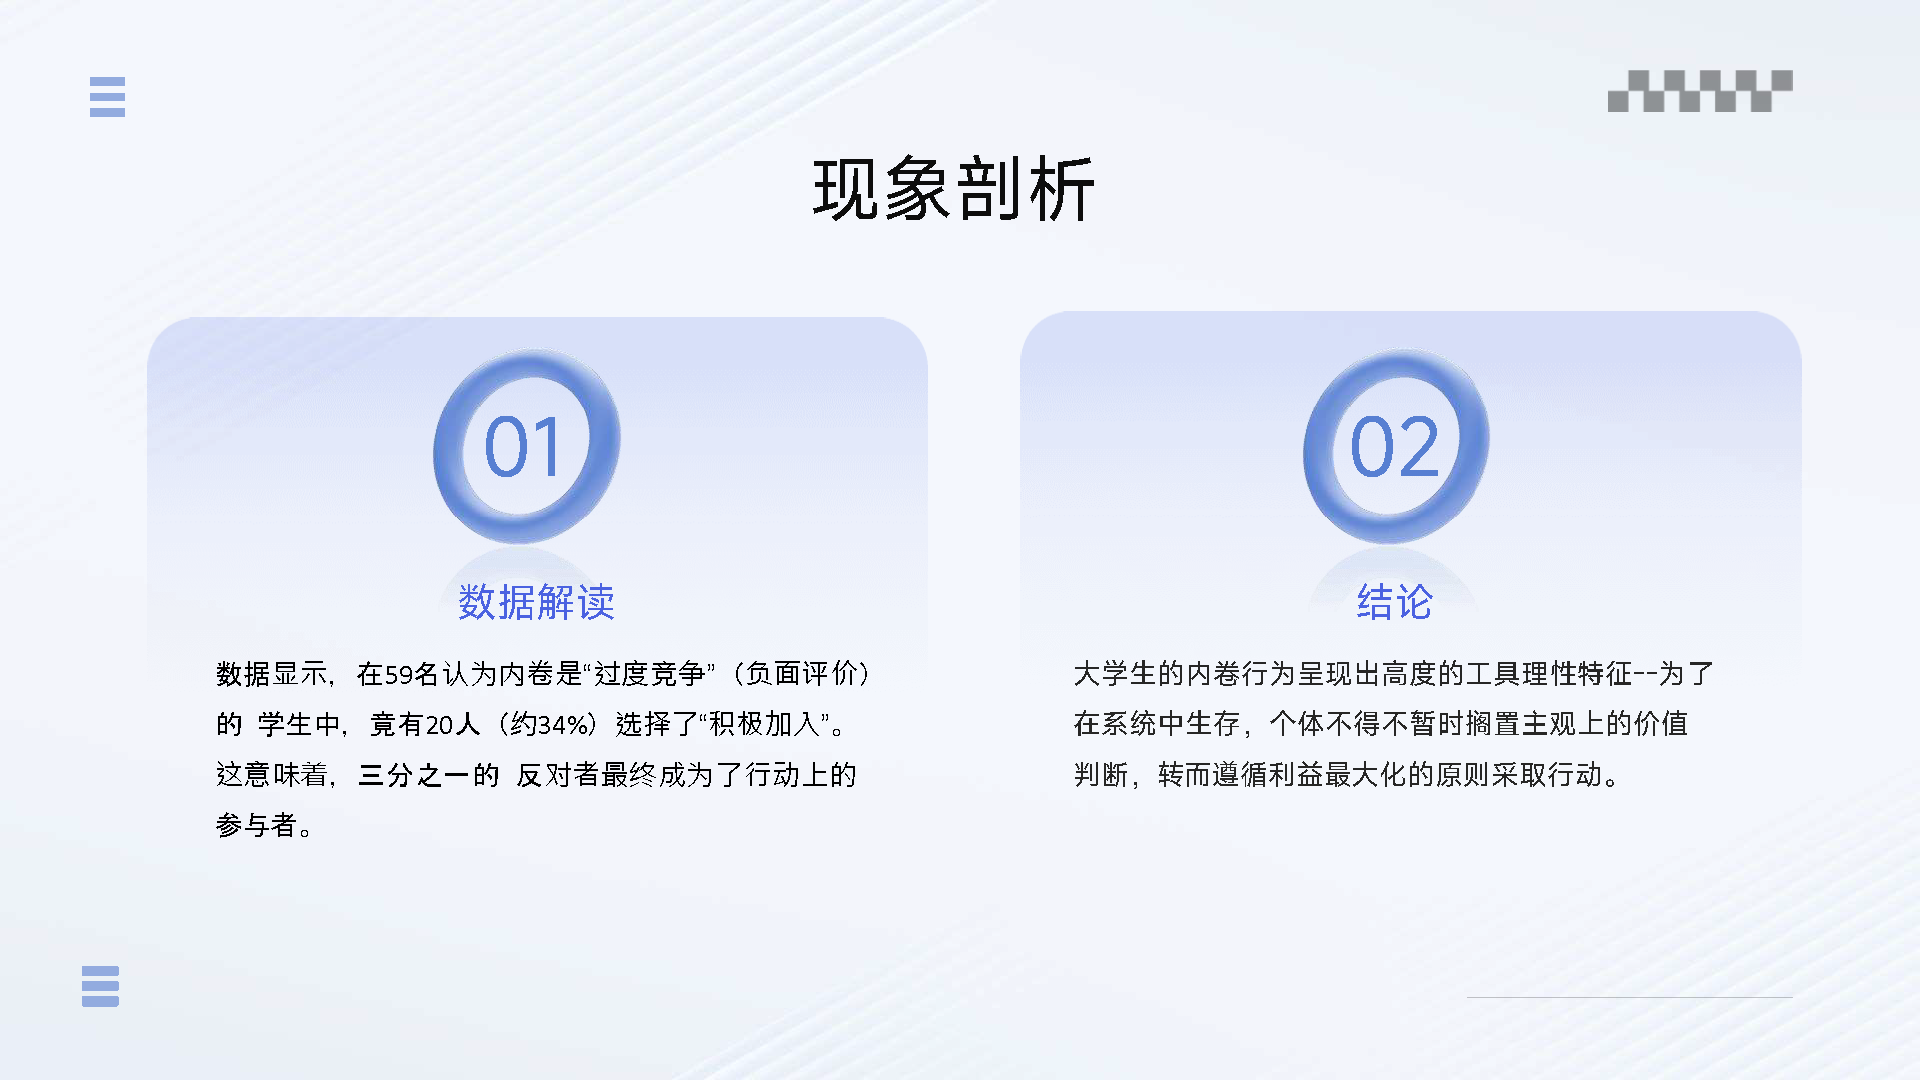
\includegraphics[width=\linewidth]{figure/image/image_页面_27.png}
\end{minipage}\hfill
\begin{minipage}[t]{0.49\textwidth}
	\centering
	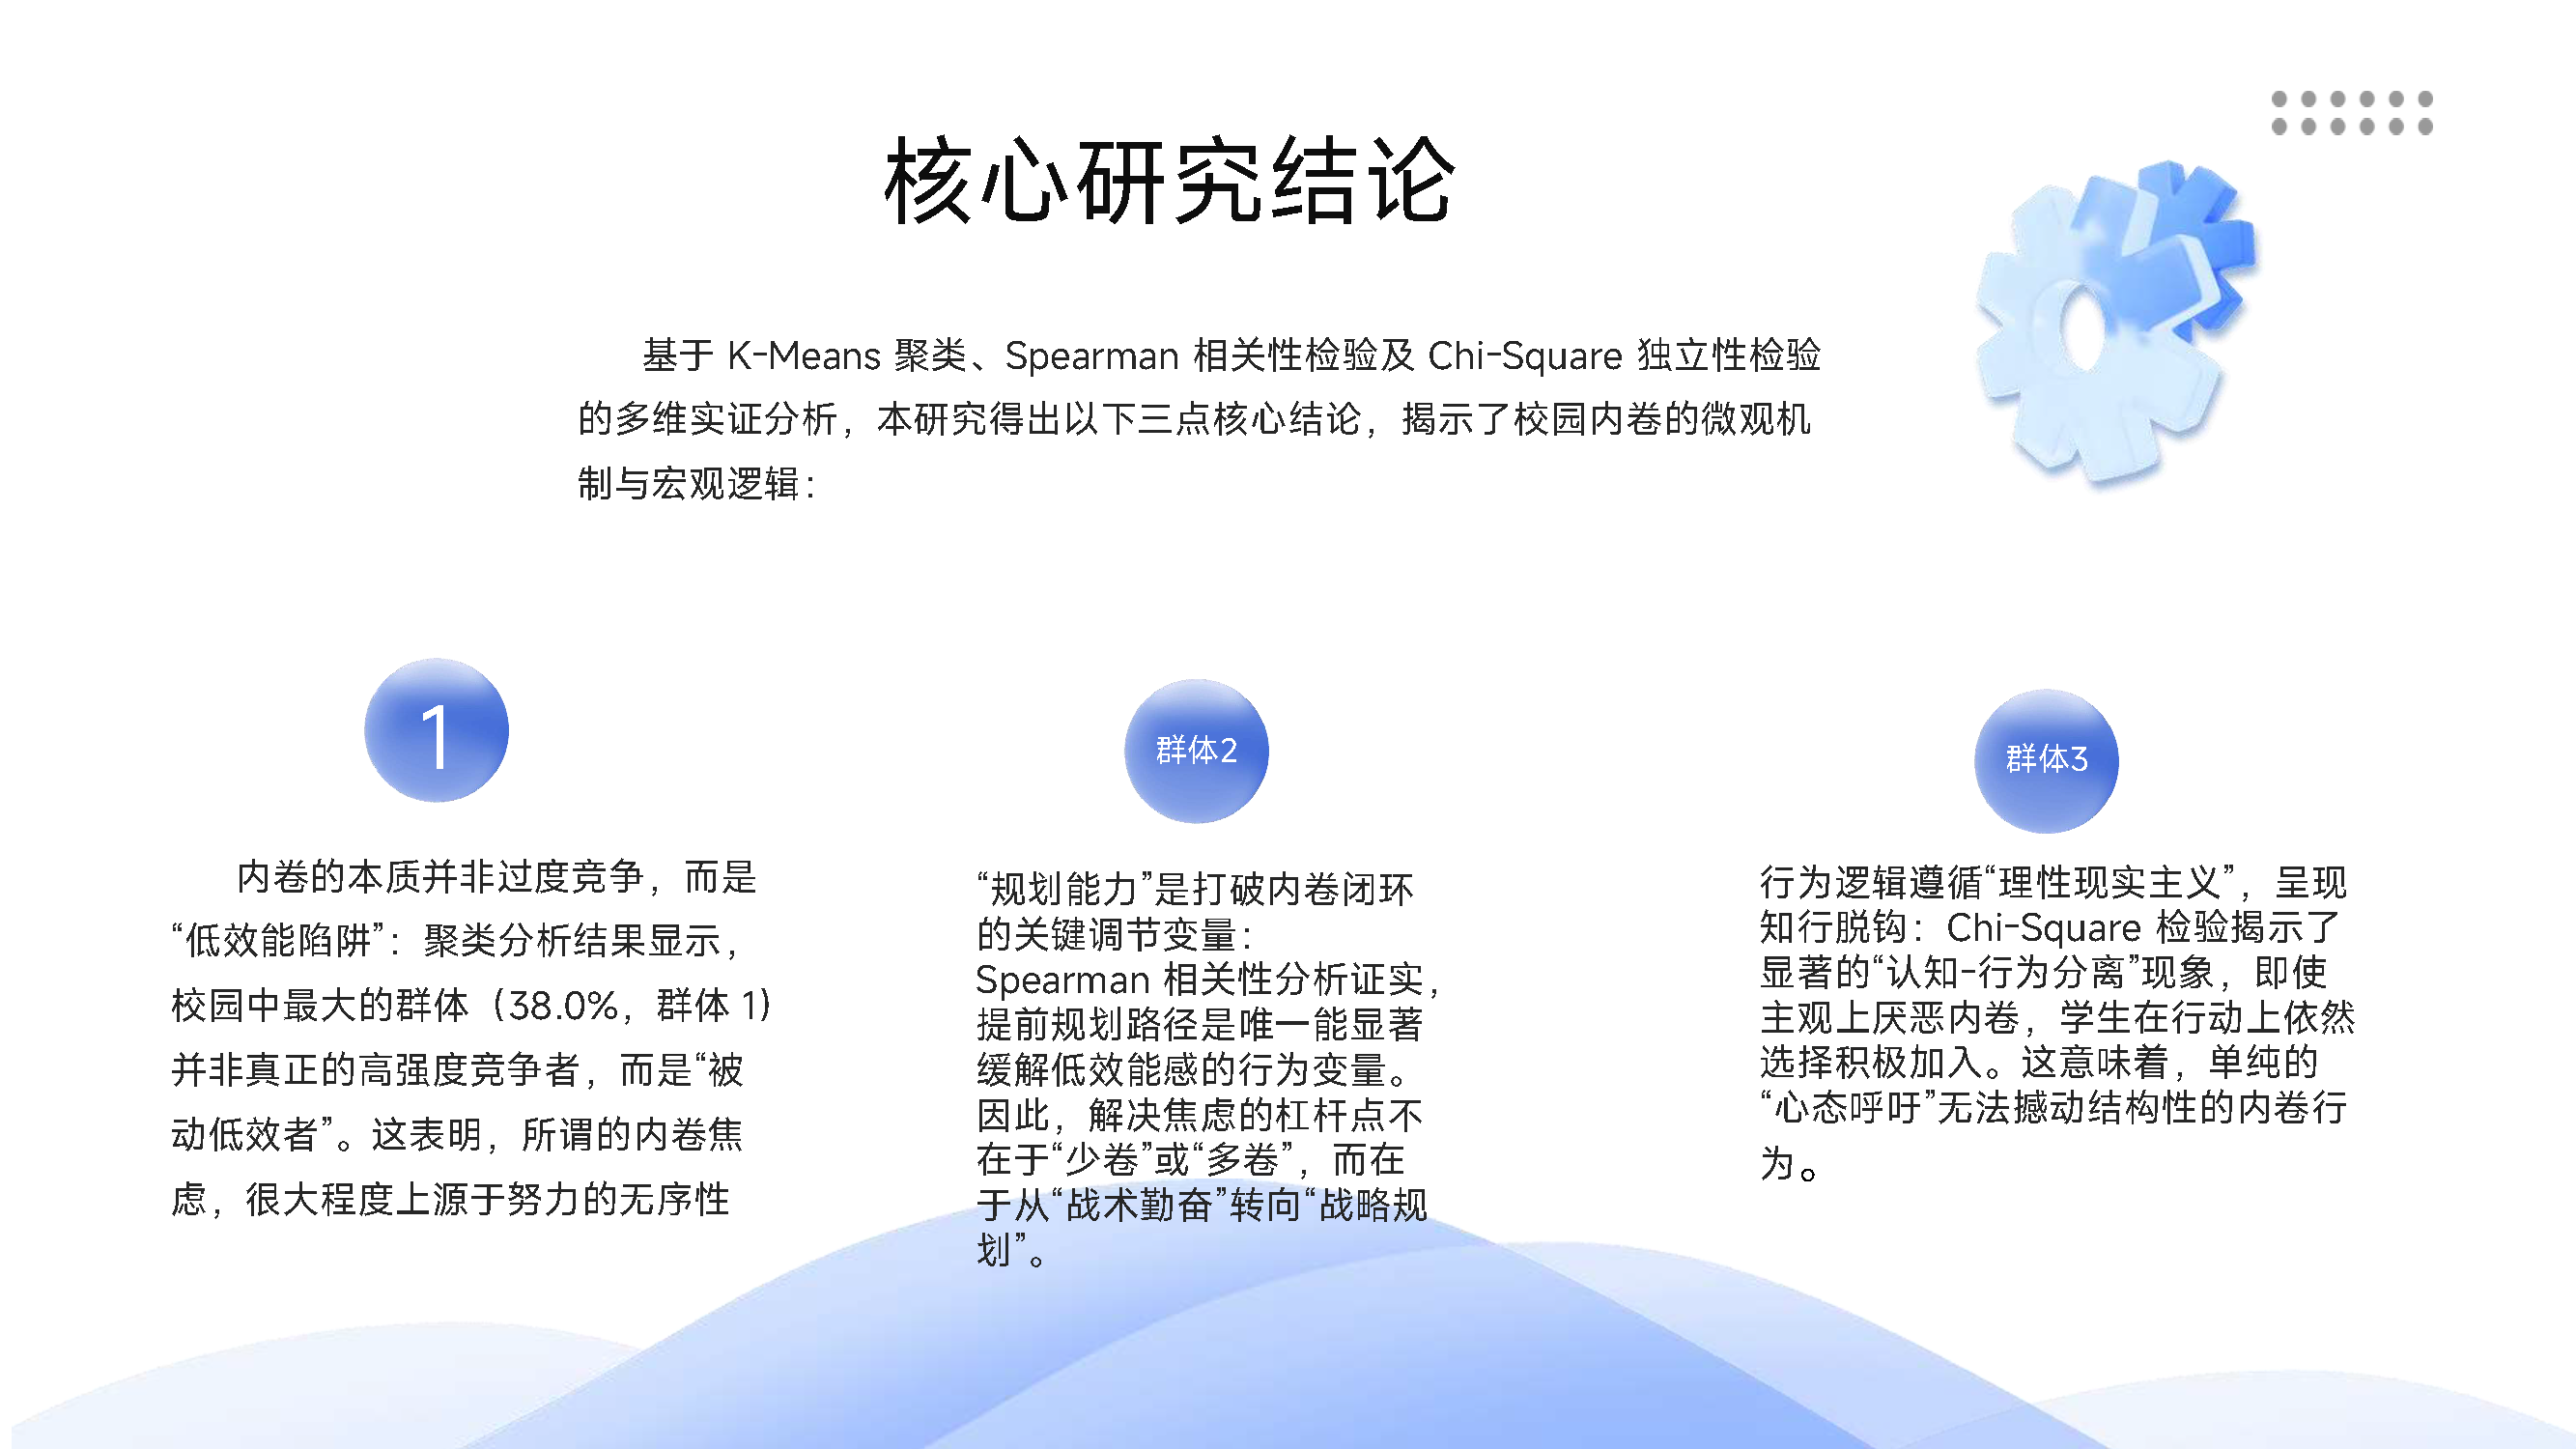
\includegraphics[width=\linewidth]{figure/image/image_页面_28.png}
\end{minipage}
\par\bigskip

\noindent
\begin{minipage}[t]{0.49\textwidth}
	\centering
	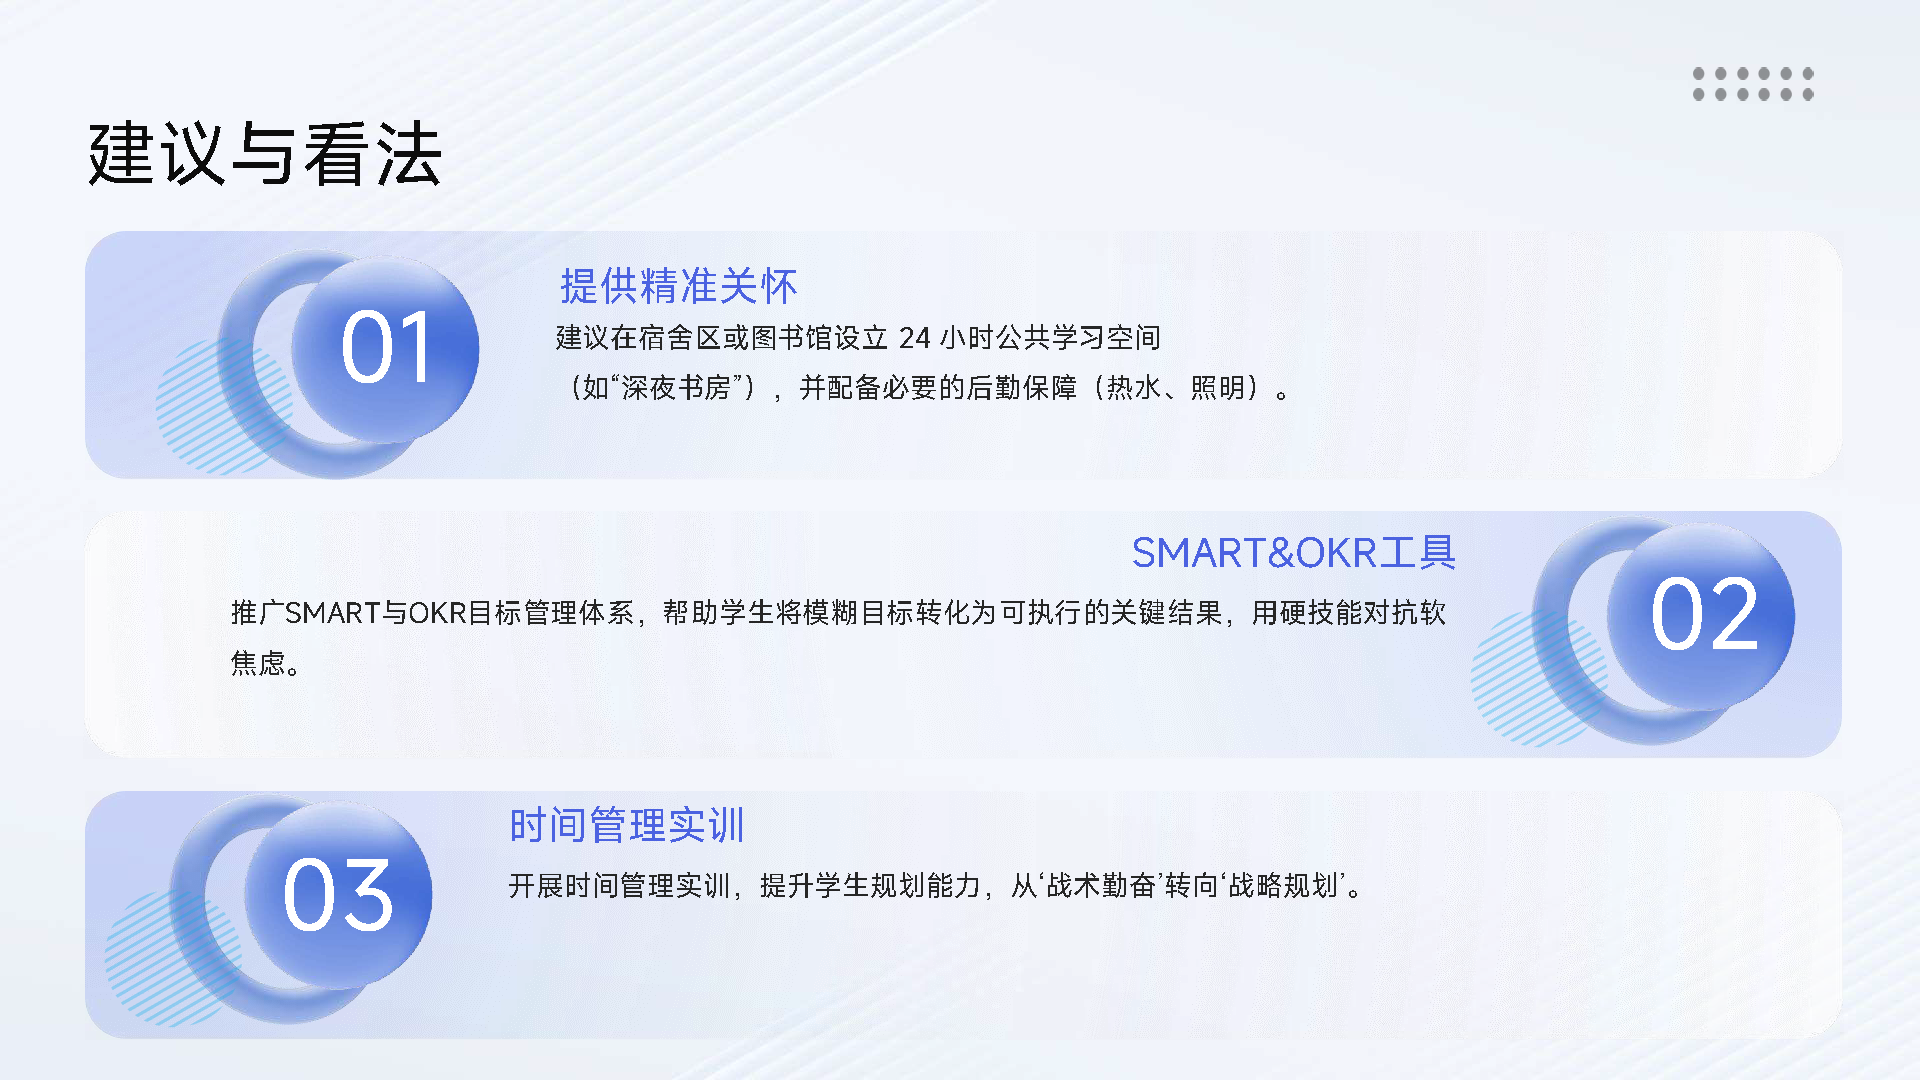
\includegraphics[width=\linewidth]{figure/image/image_页面_29.png}
\end{minipage}\hfill
\begin{minipage}[t]{0.49\textwidth}
	\centering
	
\includegraphics[width=\linewidth]{figure/image/image_页面_30.png}
\end{minipage}
\par\bigskip

\noindent
\begin{minipage}[t]{0.49\textwidth}
	\centering
	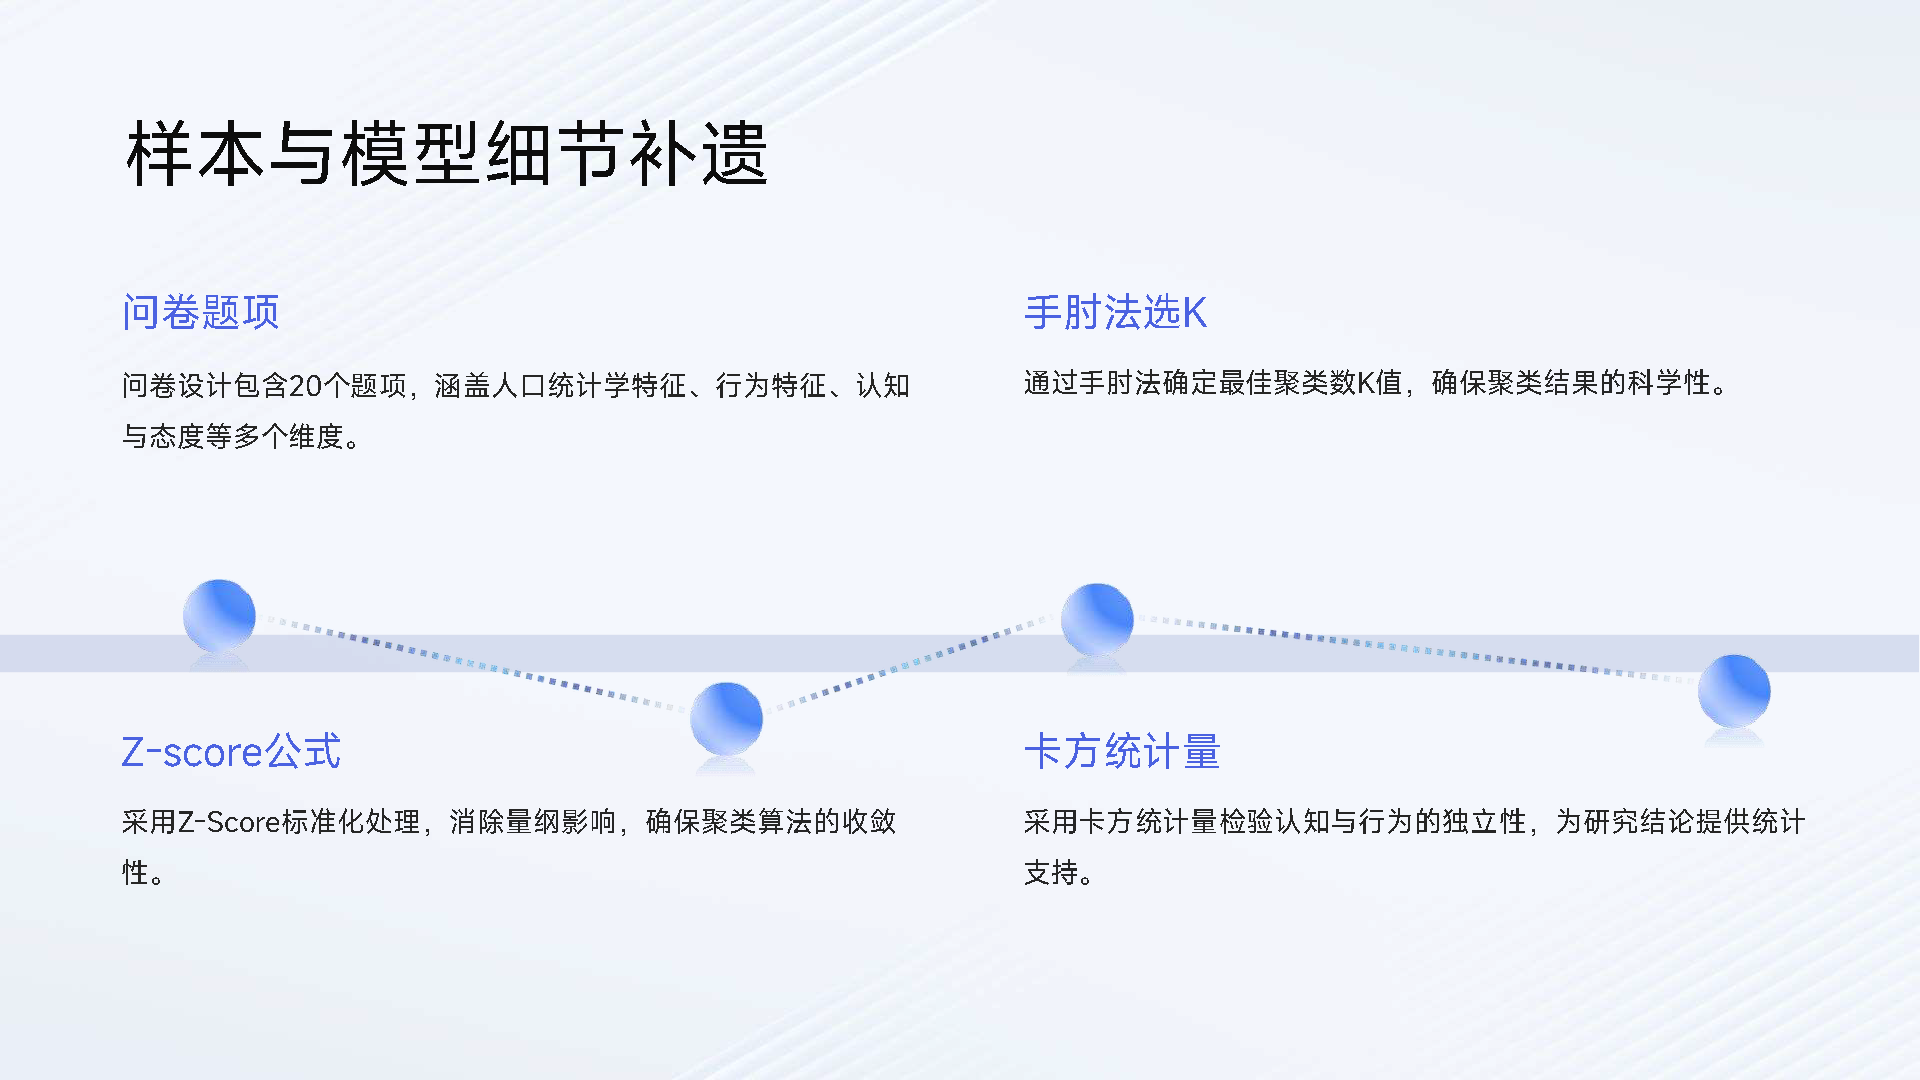
\includegraphics[width=\linewidth]{figure/image/image_页面_31.png}
\end{minipage}\hfill
\begin{minipage}[t]{0.49\textwidth}
	\centering
	
\includegraphics[width=\linewidth]{figure/image/image_页面_32.png}
\end{minipage}
\par\bigskip
\newpage
\begin{table}[htbp]
	\centering
	% 标题
	\caption*{\zihao{3}\bfseries\heiti 社会调查报告评分表}
	
	% 参数设置
	\renewcommand{\arraystretch}{1.5} % 1.5倍行高
	\setlength{\tabcolsep}{4pt}       % 略微减小列间距以节省空间
	
	% 关键配置：让表格内容垂直居中
	\renewcommand{\tabularxcolumn}[1]{m{#1}}
	
	% 表格定义
	\begin{xltabular}{\textwidth}{| >{\centering\arraybackslash}m{3.5em} | X | >{\centering\arraybackslash}m{3em} | >{\centering\arraybackslash}m{3em} |}
		\hline
		
		% === 表头 ===
		\multirow{2}{=}{\centering\textbf{序号}} & 
		\multirow{2}{=}{\centering\textbf{评\quad 价\quad 项\quad 目}} & 
		\multicolumn{2}{c|}{\textbf{评\quad 分}} \\
		\cline{3-4} 
		& & \textbf{满分} & \textbf{得分} \\
		\hline
		
		% === 内容行 ===
		1 & 
		\raggedright % 内容左对齐，阅读更自然
		能较好地理解调查任务，选题能够体现理论与实践结合的综合训练要求，实施方案难易度适宜，合理可行，能按时完成社会调查工作 & 
		15 & 
		\\
		\hline
		
		2 & 
		\raggedright
		能够自主查阅文献资料，从事调查研究，具有收集、整理、加工各种信息及获取新知识的能力，能熟练掌握和运用所学专业基本理论、基本知识和基本技能分析解决实际问题，数据真实可靠，论证充分，工作量饱满 & 
		15 & 
		\\
		\hline
		
		3 & 
		\raggedright
		数据计算结果准确，分析详实，建议合理，立足专业基础理论方法，充分结合调查背景，能够体现出一定的专业素养和创新意识 & 
		10 & 
		\\
		\hline
		
		4 & 
		\raggedright
		报告表述得当，层次清晰，格式规范，公式、图表准确、美观 & 
		10 & 
		\\
		\hline
		
		% === 总分行 ===
		\multicolumn{2}{|c|}{\textbf{总分}} & 
		50 & 
		\\
		\hline
		
		% === 签名行 (已修正) ===
		% 修改点：将原来的 |c| 改为 |@{}c@{}|，消除了导致断开的间距。
		\multicolumn{4}{|@{}c@{}|}{
			\begin{tabular}{@{} >{\centering\arraybackslash}m{5em} | m{15em} | >{\centering\arraybackslash}m{3.4em} | m{7.6em} @{}}
				% \rule{0pt}{3.5em} 用于撑开行高
				\rule{0pt}{0.5em} \textbf{教师签名} &  & \textbf{日期} &  \\
			\end{tabular}
		} \\
		\hline
		
	\end{xltabular}
\end{table}


\end{document}